%!TEX root = ../physical-olympics-2.tex
\chapter{静电学}


\section{电荷与电场}

\subsection{电磁相互作用与电荷}
物质若携带\emph{电荷}(charge),\,则可以发生\emph{电磁相互作用}(electromagnetic interaction).\,在经典情形下理解为电荷受到一个力.\,我们先研究\emph{静电学}(electrostatics),\,它要求受力物体与施力物体\footnote{实际上物理上不允许超距的施力物体,\,施力物体就是局域的电场.}都处于静止状态,\,或者认为一切电荷都处于静止状态.

电荷分正负,\,阴阳激荡.

作为协变电磁场理论的基本要求与实验规律,\,电荷是一个参考系不变的标量,\,微观地看电荷具有\emph{量子化}(quantized)的奇妙特性\footnote{与磁单极子的存在与量子化有关.}.\,质子的质量与电子的质量没有简单的整数比关系,\,但电荷量确实严格相反.\,如果设想两者电量有着微小差异,\,那么构成自然界的原子也就携带了一个能够传递远程相互作用的库仑力,\,从而导致自然界的不稳定\footnote{是的,\,这种思考方式就是\emph{人择原理}(antropic principle).}.\,而\emph{质子}(proton)的电量被定义为\emph{基本电荷}(elementary charge)\footnote{这个值是2018新国际标准单位制提出的规定值.}:
\[e=1.602176634\pow{-19} {\rm C}\]

实际上今天我们知道,\,电荷量的量子化单位实际上更小,\,至少是\(\dfrac{1}{3}e\),\,夸克的电量就是这个电量的一倍或两倍,\,可正可负.\,而\emph{电子}(electron)带一个单位的负电荷.\,当然,\,特殊场合还会有带一个单位正电荷的\emph{正电子}(positron)和一个单位负电荷的\emph{反质子}(anti-proton)甚至它们组成的反物质.\,\emph{中子}(proton)是不带电的.

\begin{wrapfigure}[16]{o}[-10pt]{7cm}
\centering
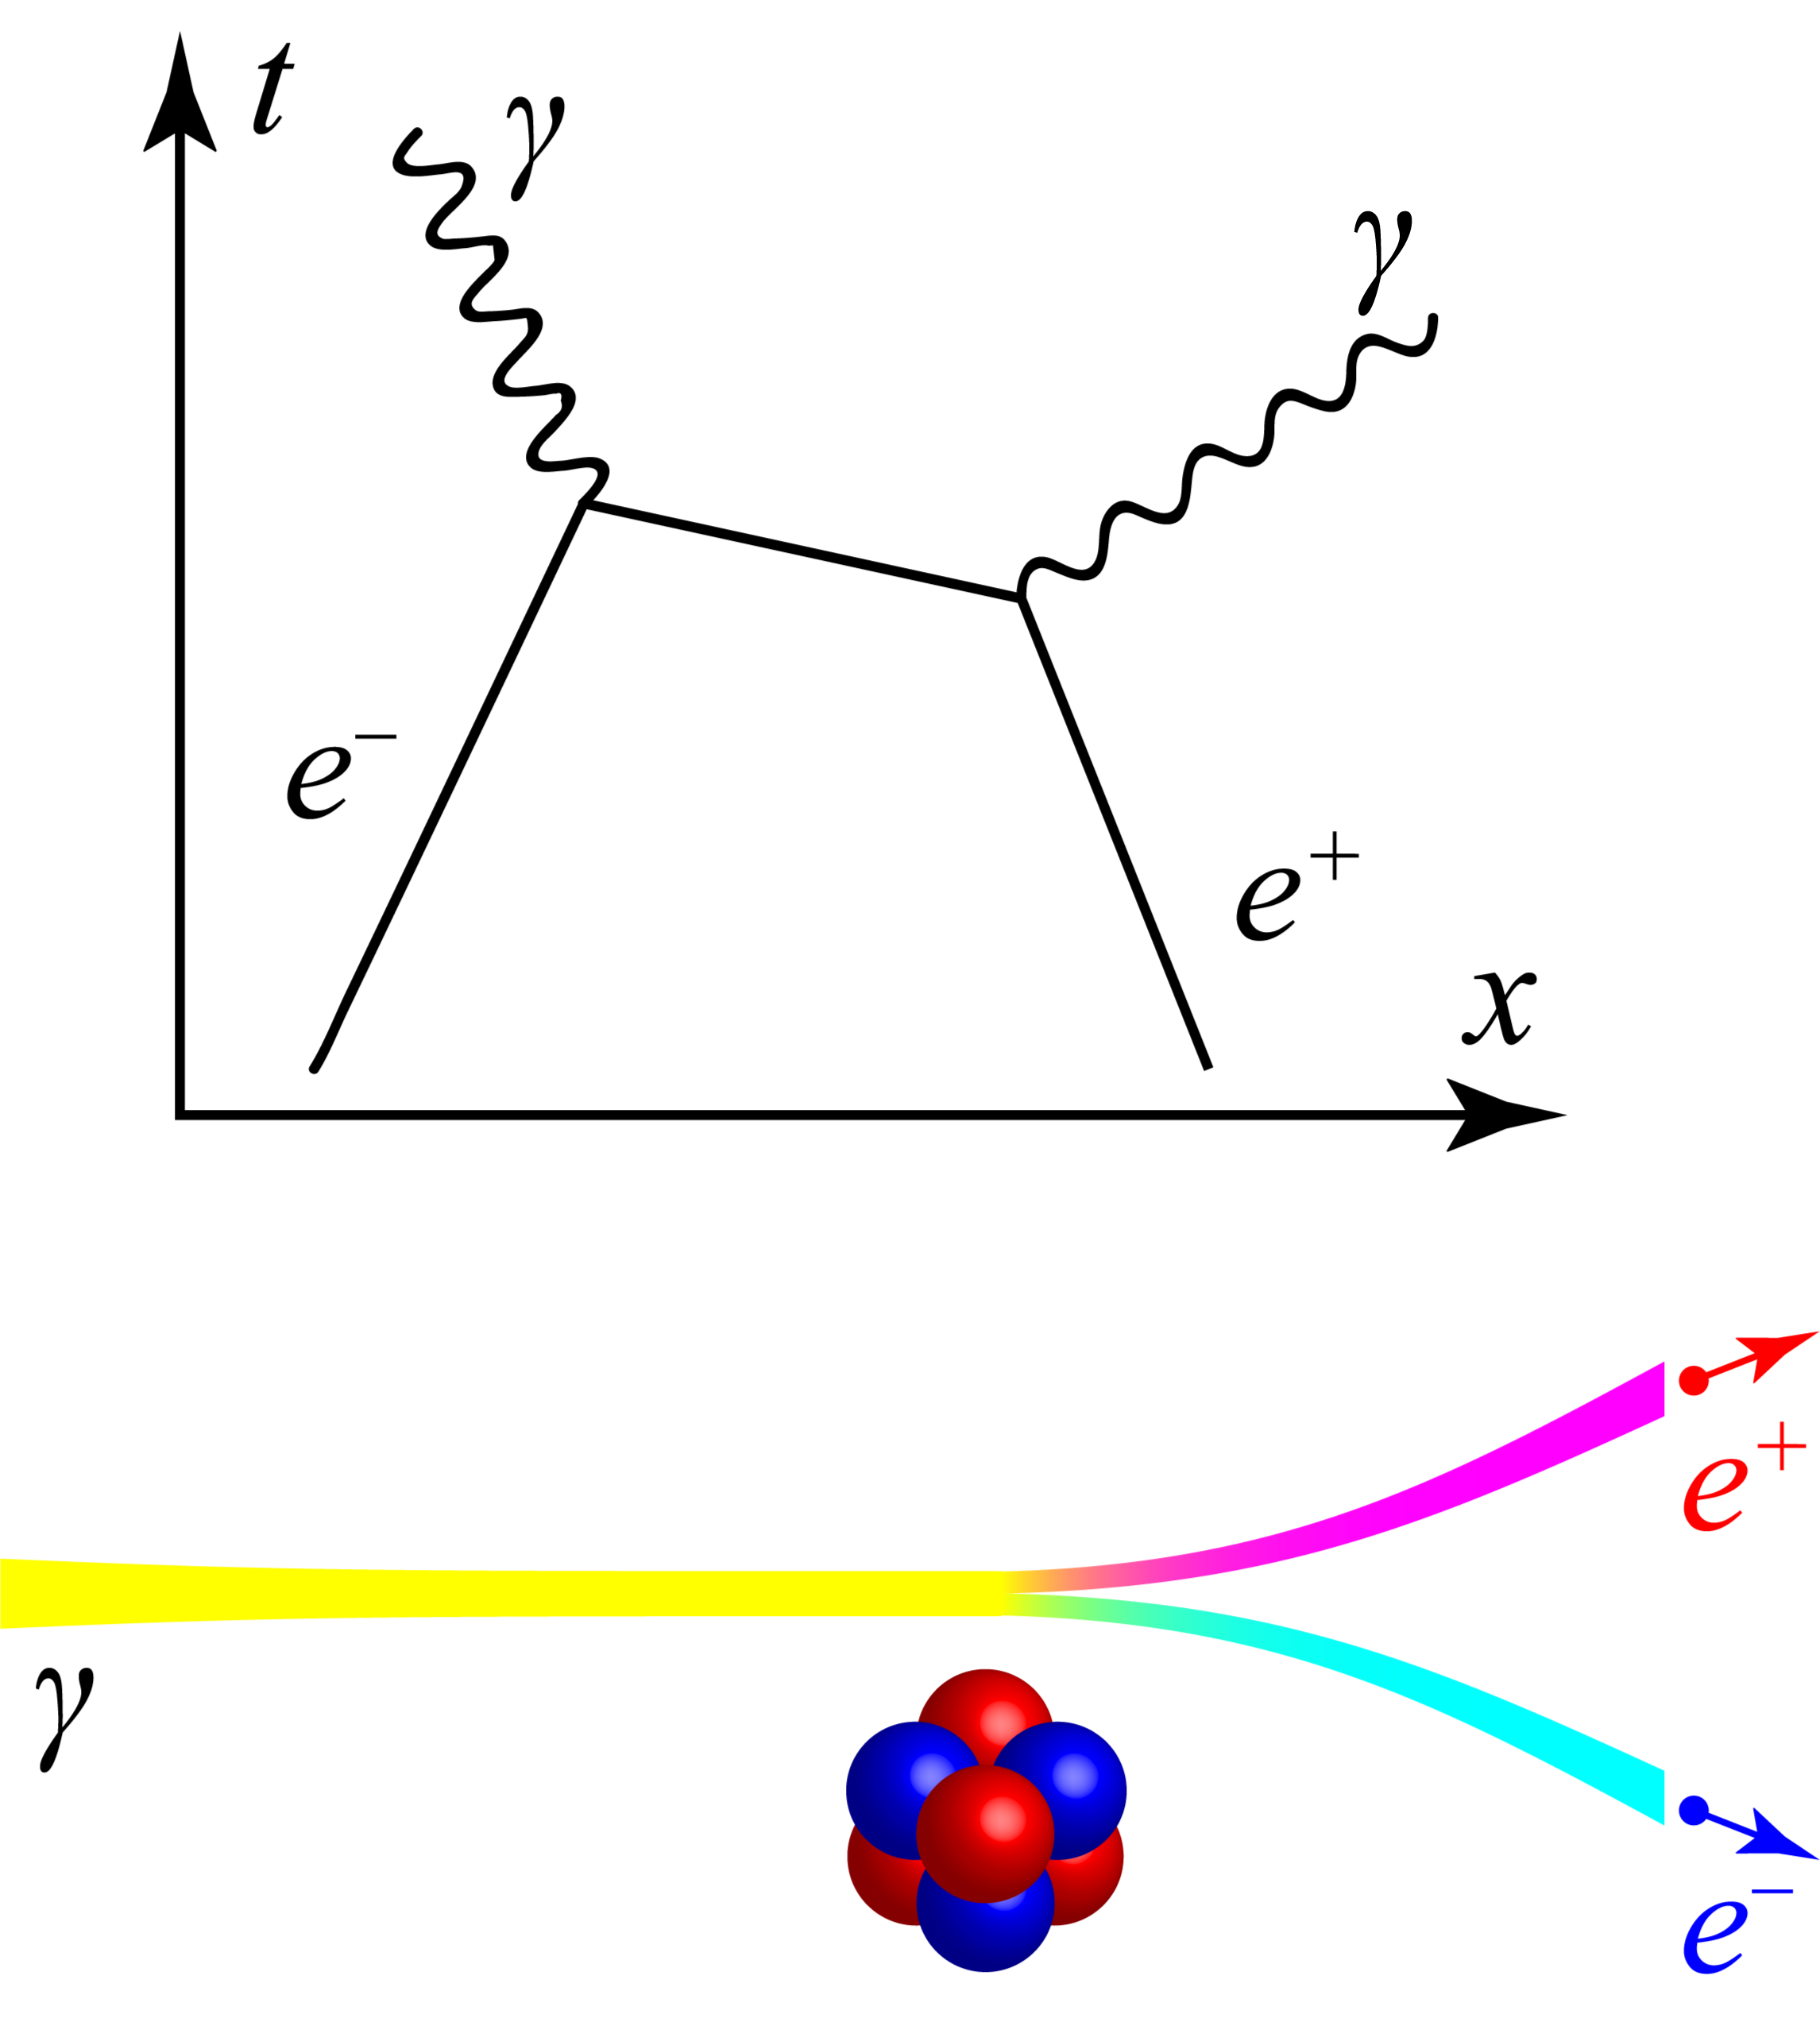
\includegraphics[width=7cm]{image/7-1-1.png}
\caption{电子对湮灭与产生}
\end{wrapfigure}
电荷如同静质量,\,是基本粒子的基本属性.\,它只能随着基本粒子运动,\,没有相互作用时不能被创造与消灭.\,在存在电磁相互作用时电荷可以被创造与消灭,\,典型的过程如电子与正电子\emph{湮灭}(annihilation)为两个光子或高能光子在原子核附近\emph{产生}(production)电子正电子对.\,这些过程电荷的代数和守恒,\,其实现要求反物质与相对论性运动的存在.\,在经典情形下有严格的\emph{电荷守恒定律}(charge conservation),\,电荷可以流动形成电流,\,但流动的过程中电荷的总量不能发生改变.\,我们总是计算一定体积内的电荷代数和:
\[\ud Q=\sum_i{n_i q_i}\ud V\]

其中\(n_i\)是第\(i\)种基本构成粒子的数密度,\,\(q_i\)是这种基本粒子的带电量.\,\(\ud V\)则为微元体积.\,而上式也被写为:
\[\ud Q=\rho \ud V\quad;\quad \rho=\sum_i{n_i q_i}=\sum_i \rho_i\]

\subsection{库仑定律}
\emph{库仑定律}(Coulumb's law)用于描述真空中的两个孤立静止点电荷之间的相互作用力:
\[\bs{F}_{12}=\ke\frac{q_1q_2}{r^2}\bs{e}_{12}\]

其中系数\(k_e=\dfrac{1}{4\pi \varepsilon_0}\approx 8.99\pow{9}{\rm N\cdot m^{-2} \cdot C^{-2}}\)为库仑常数.

\begin{wrapfigure}[11]{o}[-10pt]{7cm}
\centering
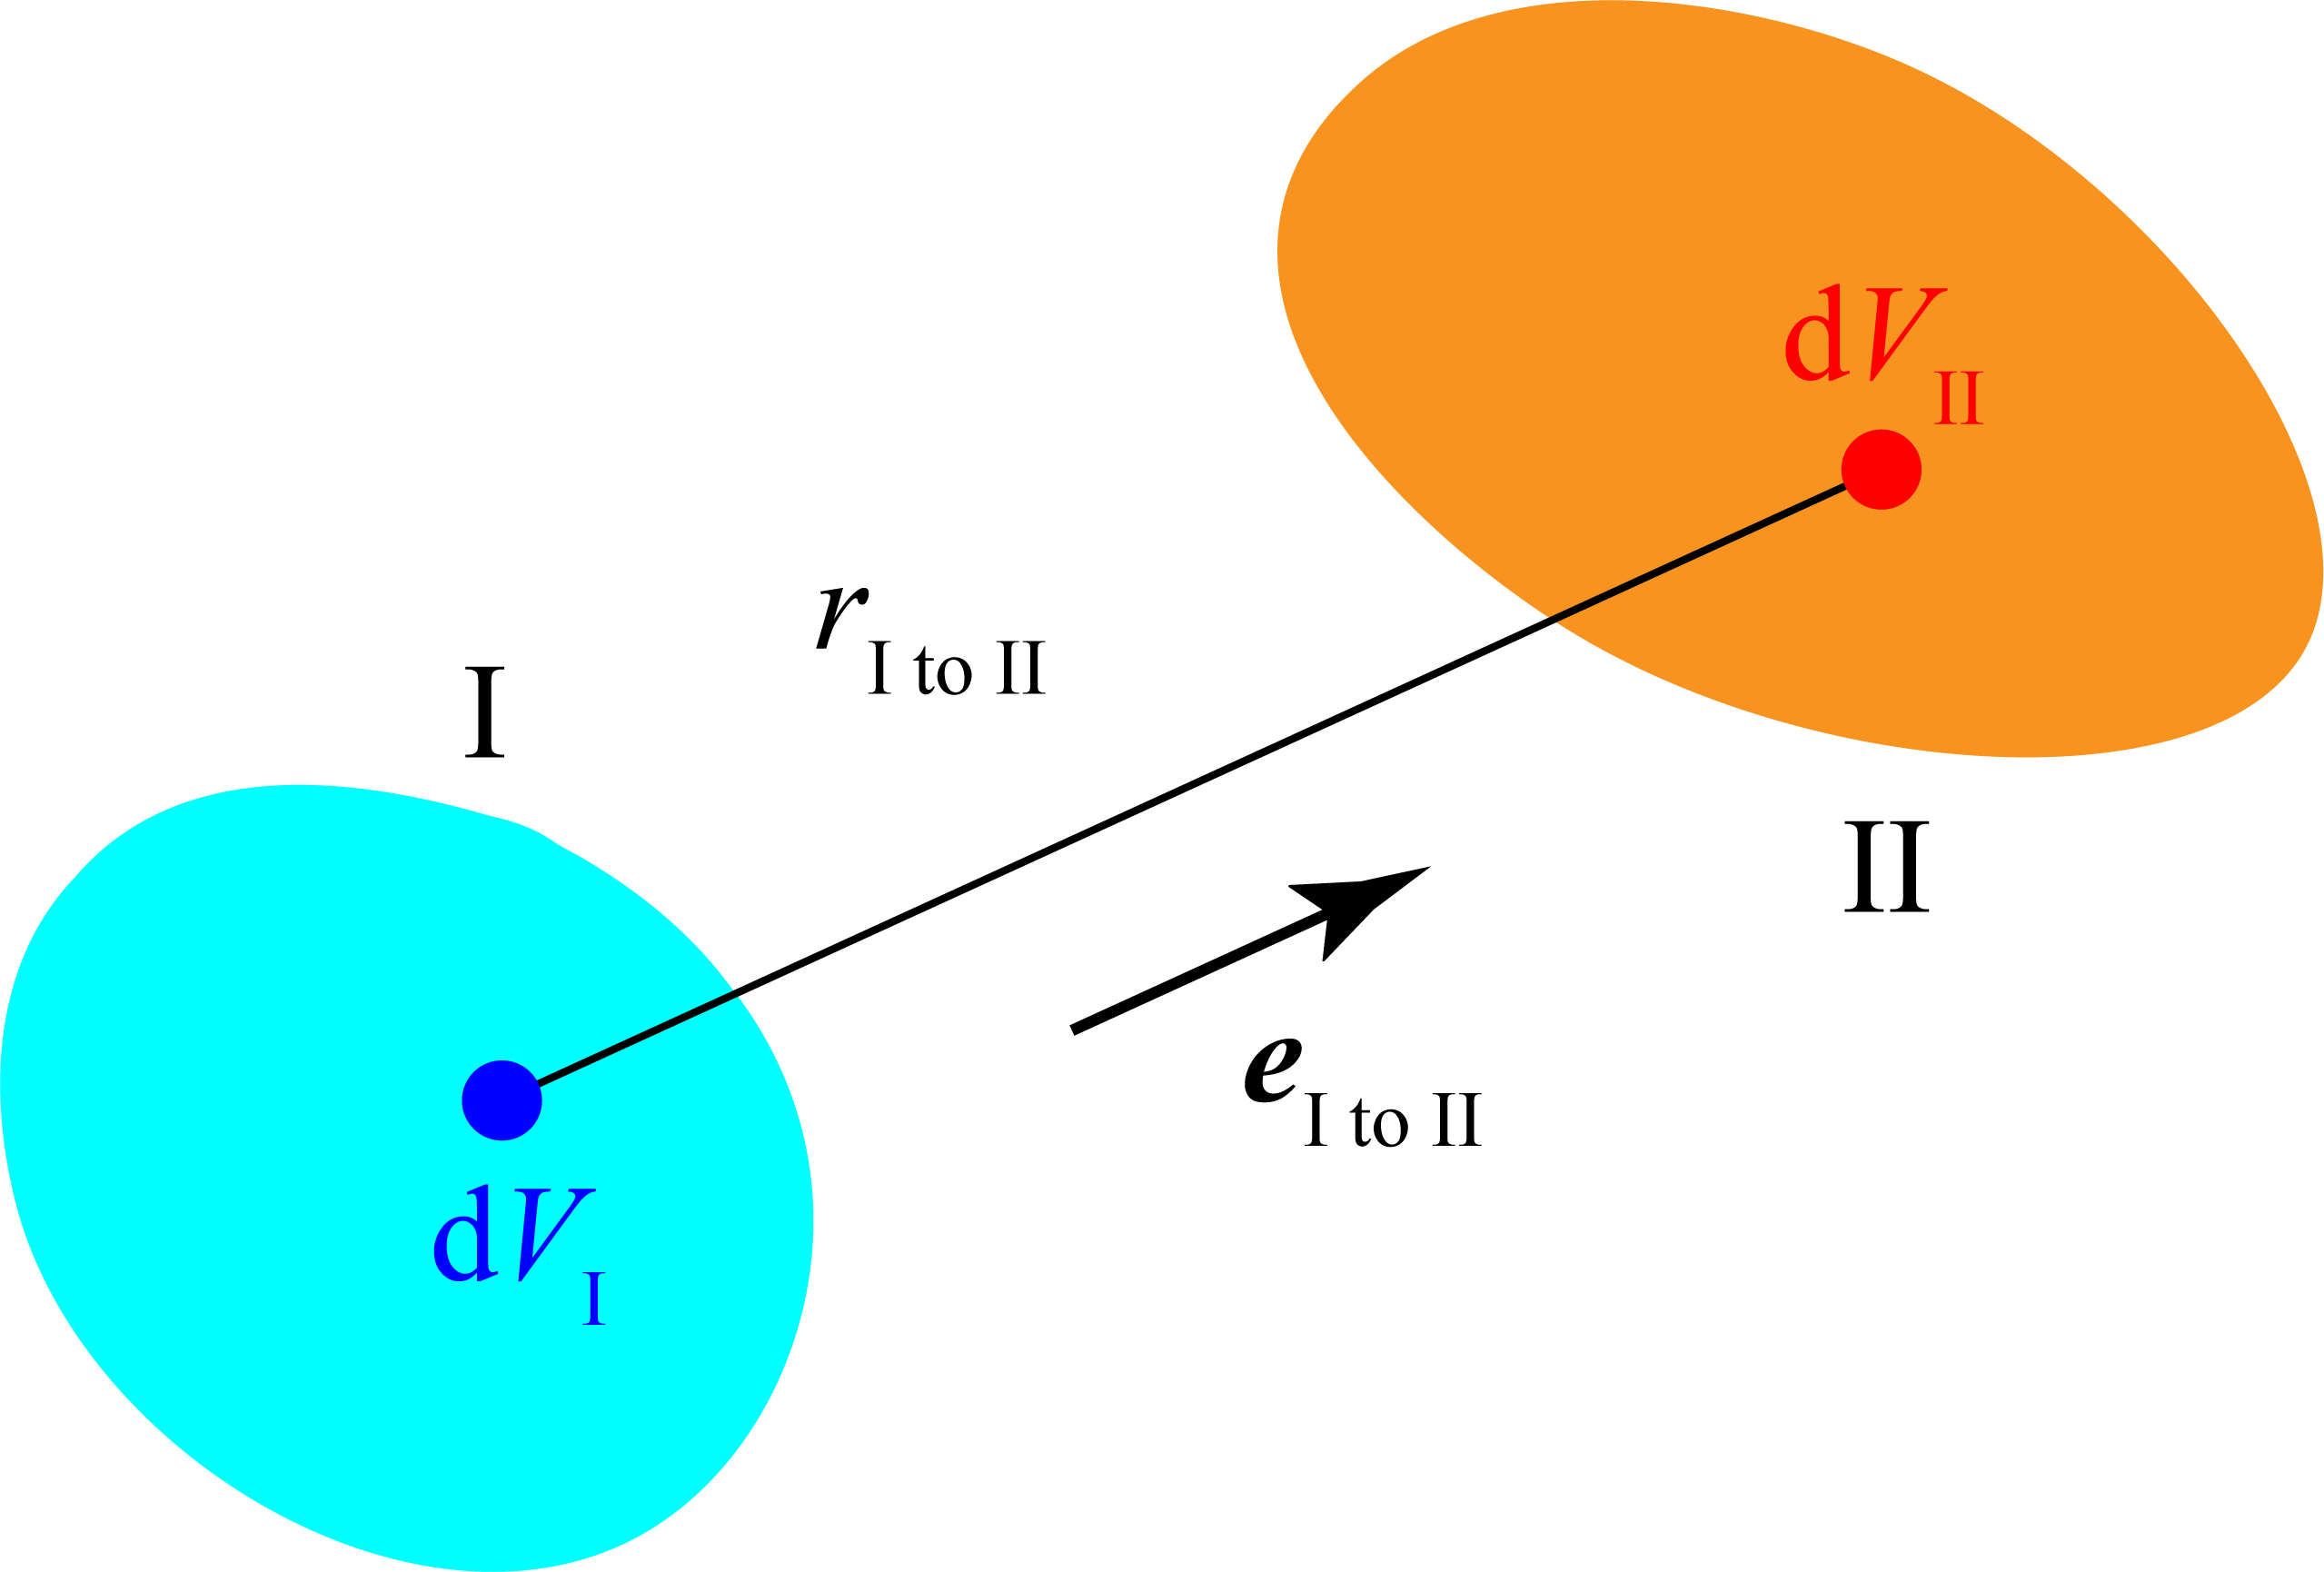
\includegraphics[width=7cm]{image/7-1-2.png}
\caption{电荷体系间的相互作用力}
\end{wrapfigure}
库仑定律是整个电磁学最基本的公理.\,其他所有规律或多或少都可以理解为库仑定律与自洽的物理概念体系的推论.\,库仑定律的特征是:

1.{\hei 平方反比(inverse-square law)}:\,与万有引力相似,\,与强相互作用与弱相互作用不同,\,荷之间的相互作用力遵从平方反比律.\,这一点使得此相互作用成为\emph{长程}(long range)相互作用,\,长至\(10^7{\rm m}\),\,短至\(10^{-17}{\rm m}\),\,库仑定律被证明是有效的.\,更短的距离下则由于量子场论的原因而使得基本电荷量的值上升,\,但基本的规律仍然不变.

2.{\hei 叠加原理(superposition principle)}:\,力与电荷成正比,\,而电荷在概念上可以作为标量线性叠加,\,说明了力的叠加本性.\,一个复杂电荷系统(包括构成介质的电荷)可以用连续的电荷密度描述:
\[\ud Q=\rho \ud V\]
	
那么两部分电荷之间的相互作用力为:
\[\bs{F}_{\rm I\,to\,II}=\ke\int\limits_{V_{\rm II}}\rho(\bs{r}_{\rm II})\int\limits_{V_{\rm I}}\frac{\rho(\bs{r}_{\rm I})}{r_{\rm I\,to\,II}^2}\bs{e}_{\rm I\,to\,II}\ud V_{\rm I}\ud V_{\rm II}\]

相互作用力在定义上就是成对存在的,\,所以两部分电荷体系间的相互作用力满足牛顿第三定律:\,大小相等,\,方向相反,\,对整个体系产生的力矩的贡献为零.

\vspace{1cm}
\subsection{电场}
现代物理认为,\,狭义相对论下的时空观是正确的.\,一个重要的推论就是\emph{局域性原理}(principle of locality):\,物体仅仅被此时此刻周围的物质所影响.\,所有相互作用必须被理解为\emph{近距作用}(action upon contact)而不能是\emph{超距作用}(action at a distance).\,这是为了能与更本质的\emph{因果律}(principle of causality)相适应.\,如果物体这一时刻的状态及其改变取决于同一时刻的空间上相隔一定距离的另外一个点(类空间隔).\,那么就可以另一个点的事件称作因,\,而物体的状态与状态改变称作果.\,但类空间隔在洛伦兹变换下具有可逆性.\,也就是原则上可以在果的时空点也可以制造事件去对因的点产生影响.\,从而造成逻辑上的紊乱.\,所以我们必须规定这两个时空点间不存在因果关系,\,互相独立没有影响.

局域性原理的直接结论便是,\,在引力与电磁相互作用时,\,作为物质的\emph{场}(field)的概念的引入.\,场本是数学概念.\,在一个三维的欧几里得空间\(\mathbb{R}^3\)中,\,如果每一个点都定义了一个数(标量),\,代表某种物理量,\,物理现象可以在不同参考系,\,惯性系中观察,\,所对应的时空点的位置坐标可能发生改变,\,但特定的时空点的概念,\,和与之相结合的物理现象与描述它的这个数,\,不应该发生改变,\,称为\emph{标量}(scalar):
\[\mathfrak{f}:\quad \bs{r}\mapsto f(\bs{r})\]
\npg{0cm}
\begin{wrapfigure}[15]{o}[0pt]{6cm}
\centering
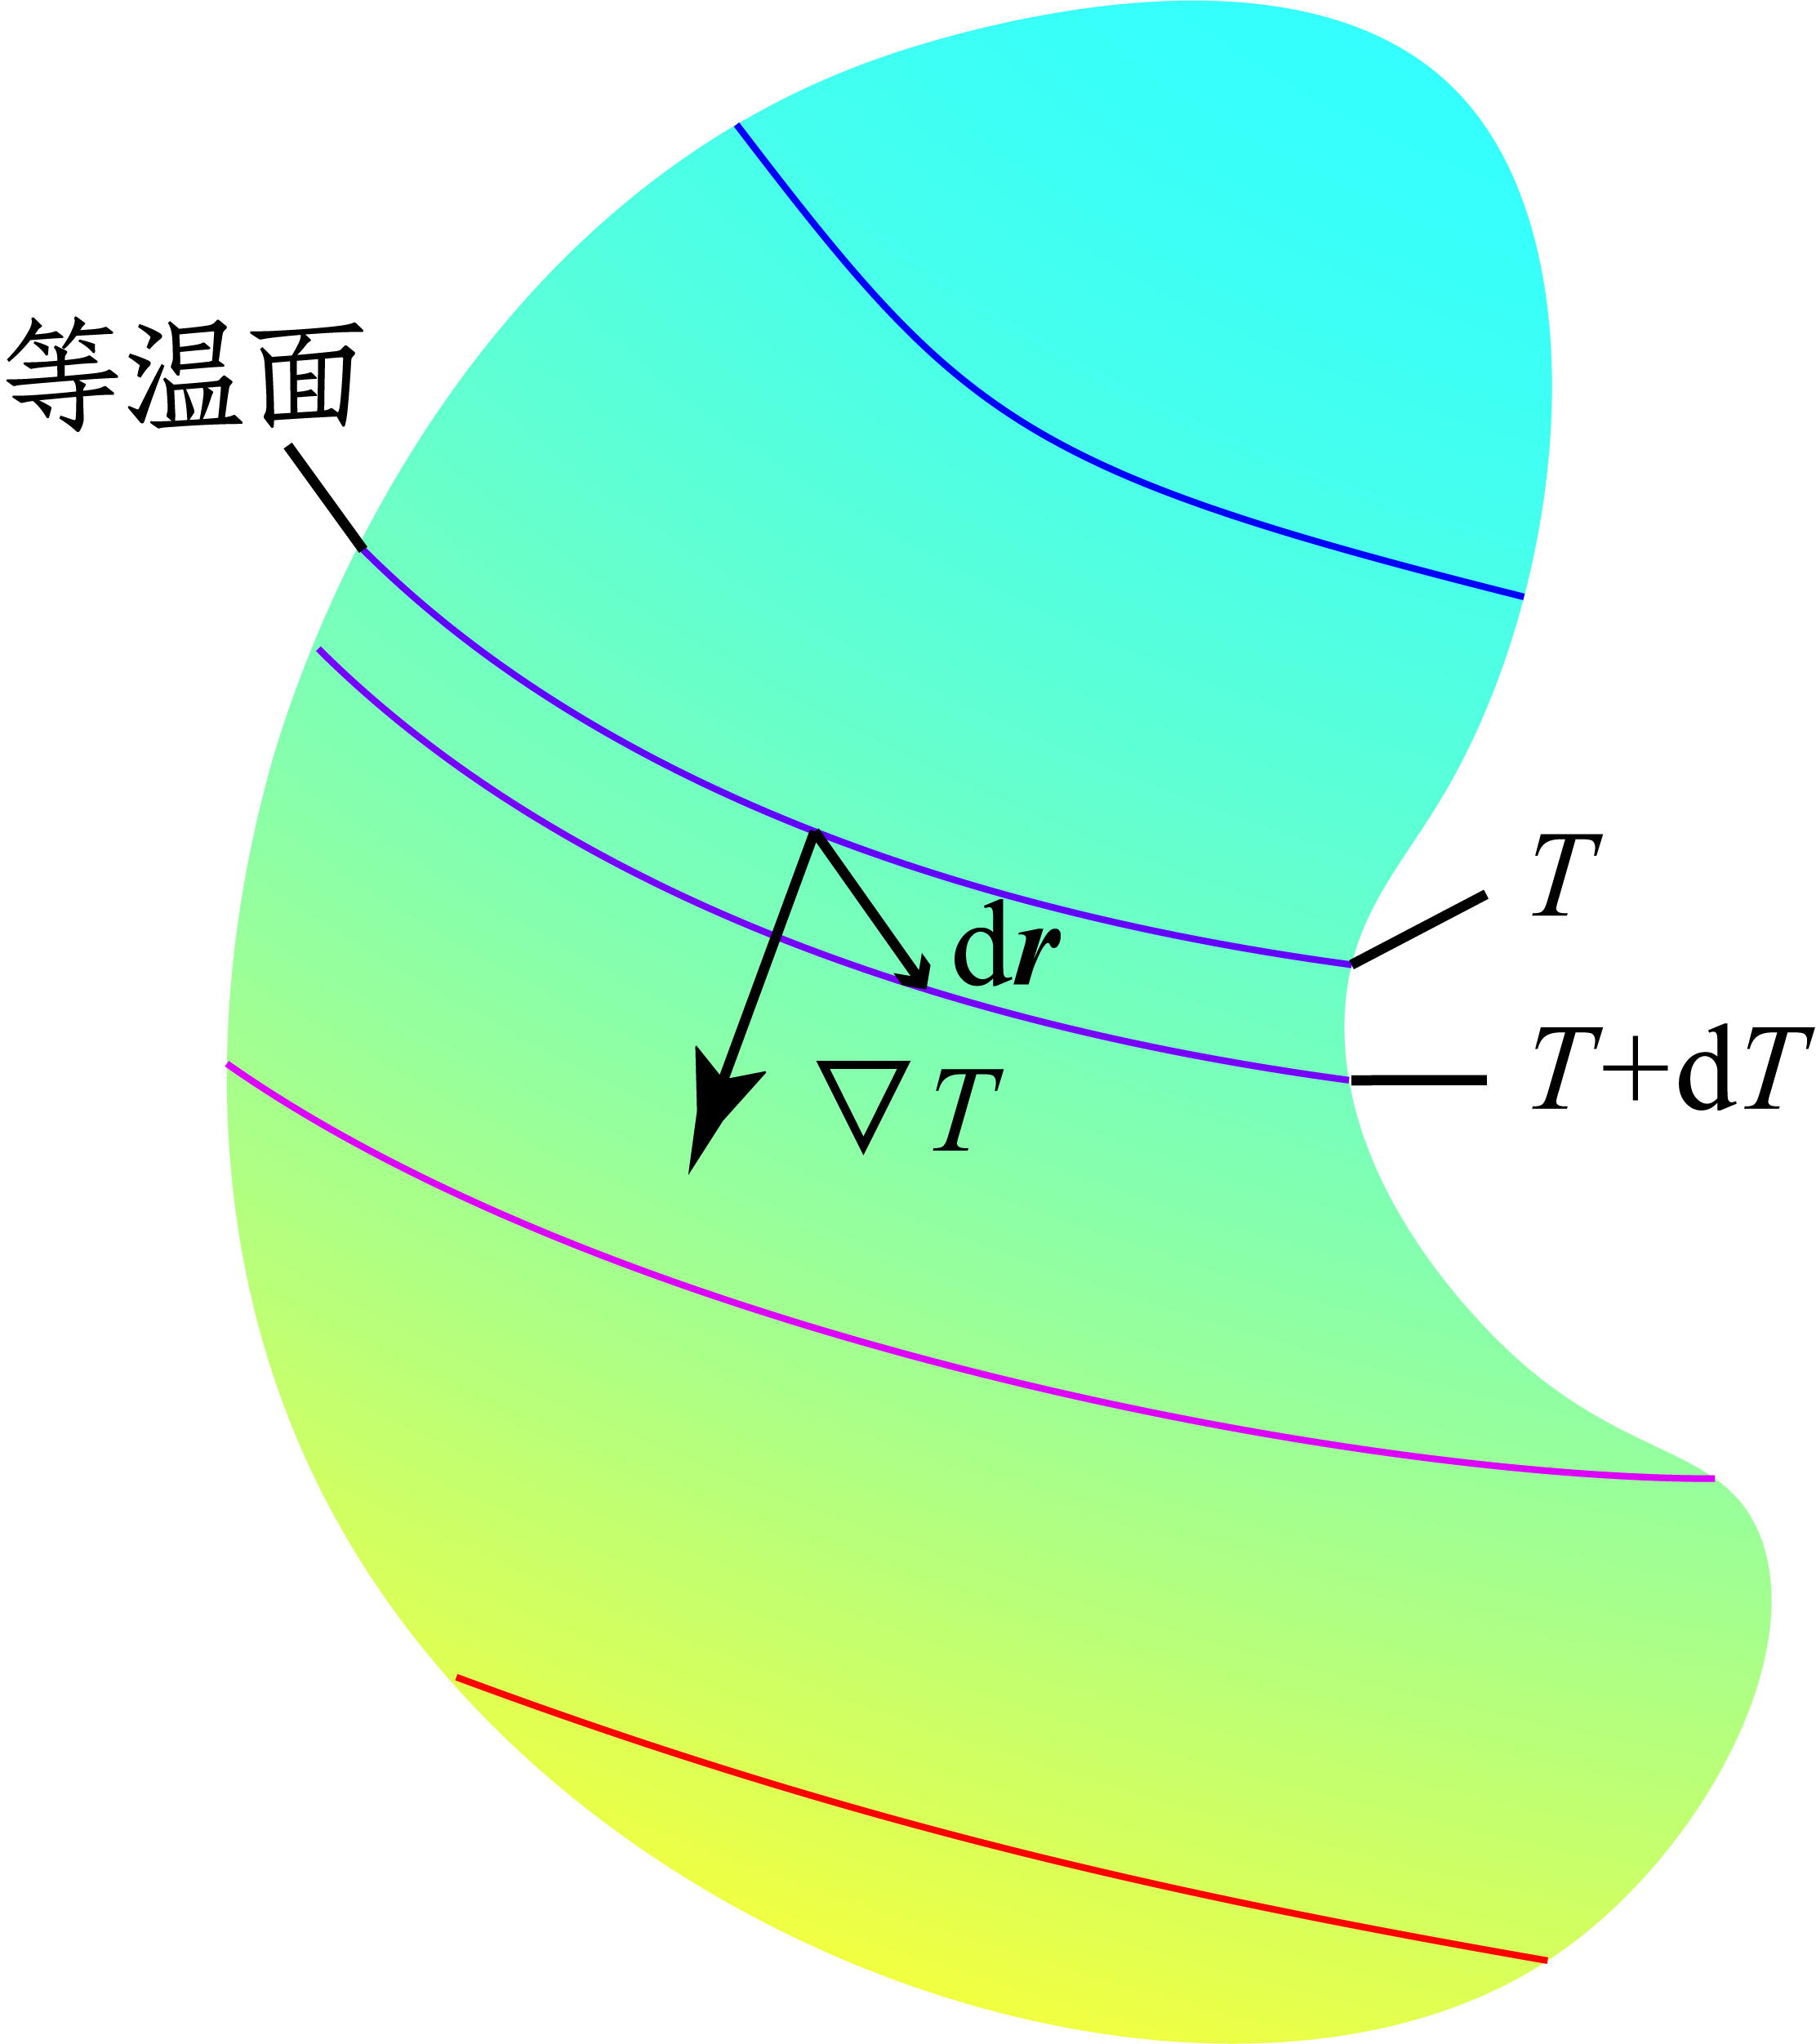
\includegraphics[width=6cm]{image/7-1-3.png}
\caption{温度场的梯度}
\end{wrapfigure}
如,\,压强场,\,温度场,\,波动的相位场,\,都是典型的标量场的例子.\,数学上定义了标量场的\emph{梯度}(gradient)来描述在一点极其附近的标量场的行为,\,它是一个矢量,\,方向是使得标量上升最快的欧几里得空间中的方向,\,大小是沿这个方向的标量变化的方向导数.\,数学上可以证明:
\[\nabla f=\frac{\partial f}{\partial x}\bs{e}_x+\frac{\partial f}{\partial y}\bs{e}_y+\frac{\partial f}{\partial z}\bs{e}_z\]

物理量在某点\(\bs{r}\)的局部,\,偏离一个\(\ud \bs{r}\)后值变为:
\[f(\bs{r}+\ud\bs{r})=f(\bs{r})+\nabla f\cdot\ud \bs{r}\]

这就是微元形式的\emph{牛顿-莱布尼茨定理}(Newton-Leibniz theorem).\,而标量场的梯度往往也具有重要的含义.\,压强场的梯度决定浮力的方向与大小(反向),\,温度场的梯度决定热传导的方向与强弱(也是反向),\,波动的相位场的梯度则决定波的传播方向与波长(波矢).

而在三维的欧几里得空间中在每一个空间点也可以引入一个\emph{矢量}(vector),\,它不占三维空间的有限体积\footnote{即,\,不同于位移矢量那样必须与三维空间中的不同点同时建立联系}而是定义在一个点上,\,可以认为是这个点上扩展出了一个新的与原三维空间坐标平行的\(\bs{e}_x-\bs{e}_y-\bs{e}_z\)坐标系.\,而这一点定义的矢量就位于这个``浓缩在一点''的坐标系中\footnote{数学术语把空间叫做\emph{微分流形}(differentiable manifold),\,而局部的矢量位于的空间叫做\emph{纤维}(fiber)或\emph{切空间}(tagent space),\,每一点都有一个这样的空间,\,合称\emph{纤维丛}(fiber bundle).}:
\[\mathfrak{F}:\quad \bs{r}\mapsto\bs{F}(\bs{r})\]

显然,\,标量场的梯度恰是一个矢量场.\,矢量不能简单理解为三个标量场的合成.\,因为在空间旋转(或时空的惯性系变化)下,\,标量应该是不变的,\,而矢量将发生与坐标系相似的旋转,\,从而三个分量之间相互转化,\,只有矢量的模长是不变的.\,另一种典型的矢量场是流体的流速场\(\bs{v}\),\,或者更普遍的,\,某种物理属性的流密度场\(\bs{j}\),\,前者定义为单位时间通过单位面积的体积,\,后者则推广为单位时间通过单位面积的某物理量\(Q\):
\[\ud Q=\bs{j}\cdot\ud A\ud t\]

在一点附近的矢量场的行为则比标量场复杂很多:
\[\bs{F}(\bs{r}+\ud\bs{r})=\bs{F}(\bs{r})+\ud \bs{r}\cdot\nabla \bs{F}\]

此处\(\nabla=\bs{e}_x\dfrac{\partial}{\partial x}+\bs{e}_y\dfrac{\partial}{\partial y}+\bs{e}_z\dfrac{\partial}{\partial z}\)可以形式地视为矢量微分算符,\,它写在上一式的后一项中实际上是在表示:
\begin{align*}
\ud \bs{F} 	&=\ud F_x \bs{e}_x+\ud F_y \bs{e}_y+\ud F_x \bs{e}_z \\
			&=(\frac{\partial F_x}{\partial x}\ud x+\frac{\partial F_x}{\partial y}\ud y+\frac{\partial F_x}{\partial z}\ud z)\bs{e}_x\\
			&\phantom{=}+(\frac{\partial F_y}{\partial x}\ud x+\frac{\partial F_y}{\partial y}\ud y+\frac{\partial F_y}{\partial z}\ud z)\bs{e}_y\\
			&\phantom{=}+(\frac{\partial F_z}{\partial x}\ud x+\frac{\partial F_z}{\partial y}\ud y+\frac{\partial F_z}{\partial z}\ud z)\bs{e}_z\\
			&=(\ud x\frac{\partial}{\partial x}+\ud y\frac{\partial}{\partial y}+\ud z\frac{\partial}{\partial z})(F_x\bs{e}_x+F_y\bs{e}_y+F_z\bs{e}_z)\\
			&=\ud \bs{r}\cdot\nabla \bs{F}
\end{align*}

而也可以把\(\nabla \bs{F}\)认为能完整描述这个矢量在该点处的一阶变化行为,\,也称为矢量的梯度,\,但它实际上由九个分量组成,\,分别描述三个分量在三个方向的变化率,\,一般写在一张数表中,\,也就是矩阵\footnote{实际上,\,形成了一个\emph{张量场}(tensor filed).\,张量将不在本部分教材的讨论范围内.}:
\[\nabla \bs{F}=\begin{bmatrix}
\dfrac{\partial F_x}{\partial x}&\dfrac{\partial F_y}{\partial x}&\dfrac{\partial F_z}{\partial x}\\[3pt]
\dfrac{\partial F_x}{\partial y}&\dfrac{\partial F_y}{\partial y}&\dfrac{\partial F_z}{\partial y}\\[3pt]
\dfrac{\partial F_x}{\partial z}&\dfrac{\partial F_y}{\partial z}&\dfrac{\partial F_z}{\partial z}
\end{bmatrix}\]

显然用这样的一个矩阵去描述矢量场在一点处的行为是代数的,\,抽象地,\,不几何直观的.\,所以我们引入两个物理上会更实用的概念.

\begin{wrapfigure}[16]{o}[0pt]{7cm}
\centering
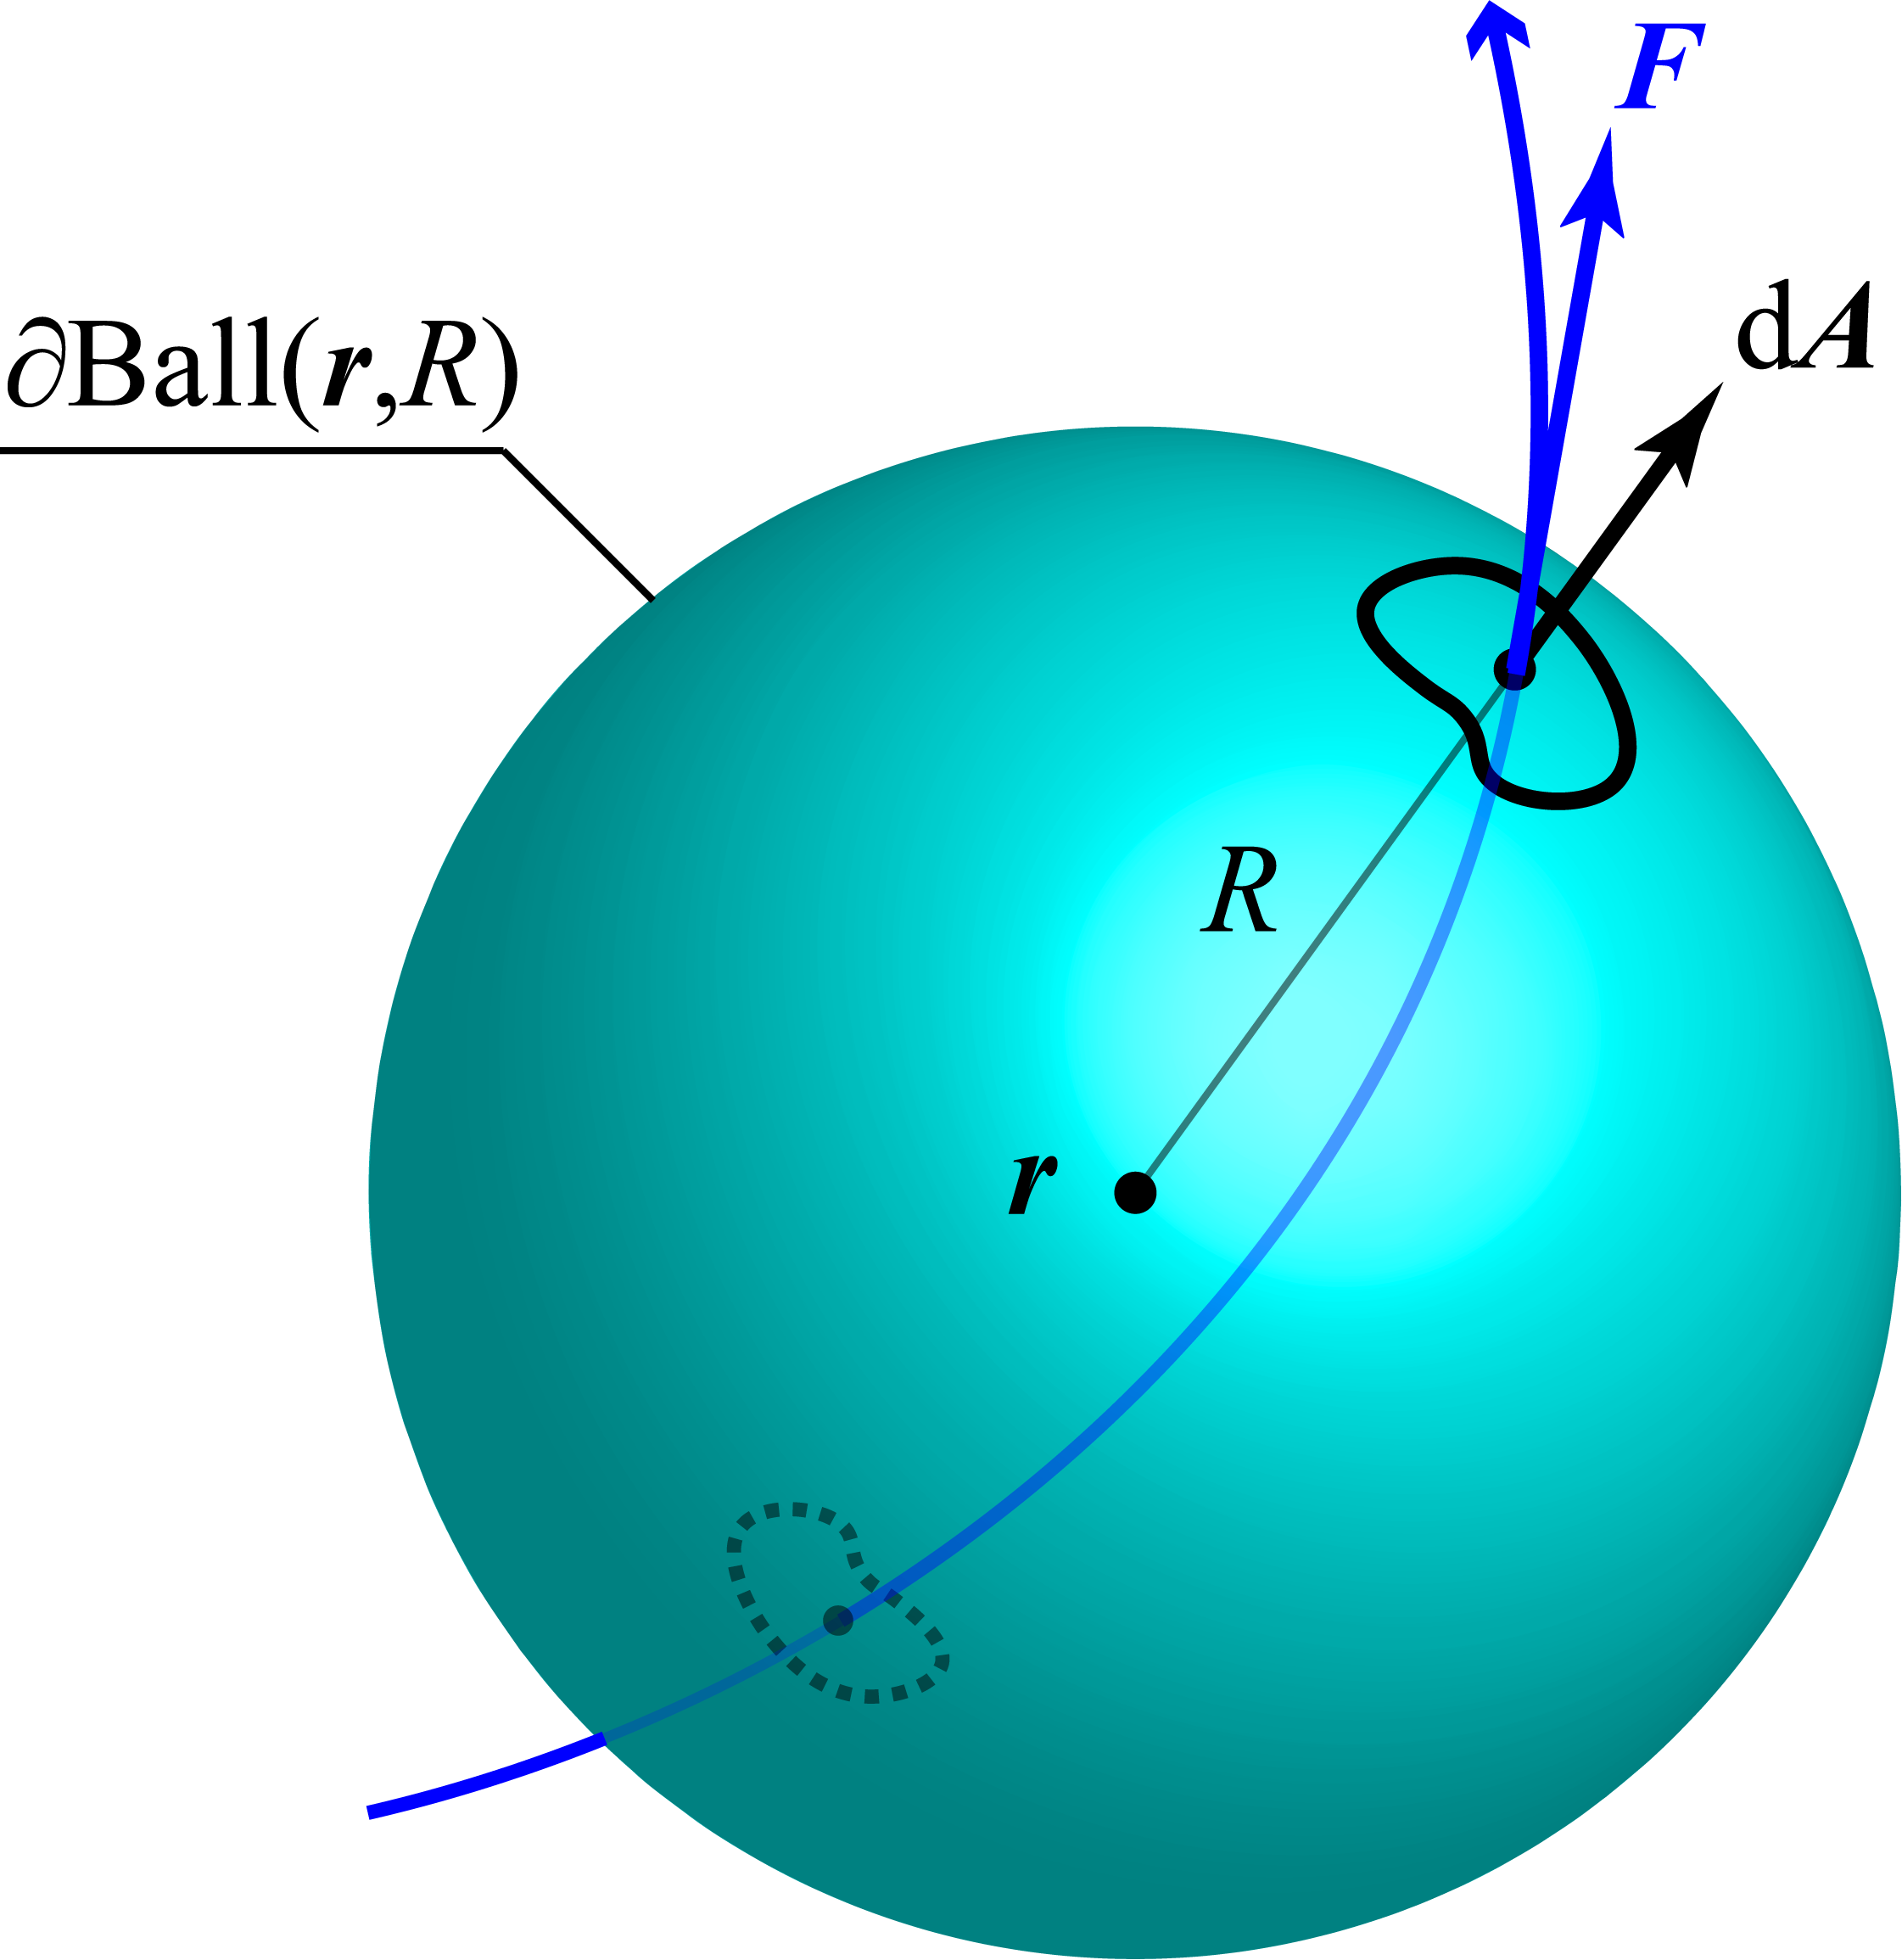
\includegraphics[width=7cm]{image/7-1-4.png}
\caption{矢量场的散度}
\end{wrapfigure}
一是矢量场的\emph{散度}(divergence),\,它是一个标量,\,定义为矢量场的源强度:
\[\nabla\cdot \bs{F}=\lim_{R\to 0}\left.\left(\oint_{\partial {\rm Ball}(\bs{r},R)}\bs{F}\cdot \ud\bs{A}\right)\right/(\frac{4}{3}\pi R^3)\]

其中\({\rm Ball}(\bs{r},R)\)表示以待研究的点为球心的,\,半径为\(R\)的球形体,\,而\(\partial {\rm Ball}\)表示它的表面.\,积分号\(\oint\)用来代表此场合下用来积分的区域是一个闭合的区域\footnote{数学上称为\emph{又闭又开}(clopen)的集合,\,表示它没有边界.}.\,积分的量称为\emph{通量}(flux),\,即矢量场与面积的电场,\,速度场情况下即单位时间通过面\(\ud \bs{A}\)的体积.\,现在对闭合的面进行积分,\,再除以面包含的体积,\,代表的是该点单位体积内产生这个矢量场的场线的源的多少,\,即源强度.\,数学上可以证明,\,它与体积以怎样的取法趋于零无关,\,如果取成与坐标系平行的长方体的形状,\,能够在坐标系下计算出它的值为:
\[\nabla\cdot\bs{F}=\frac{\partial F_x}{\partial x}+\frac{\partial F_y}{\partial y}+\frac{\partial F_z}{\partial z}\]

\begin{wrapfigure}[15]{o}[0pt]{7cm}
\centering
\vspace{0.5cm}
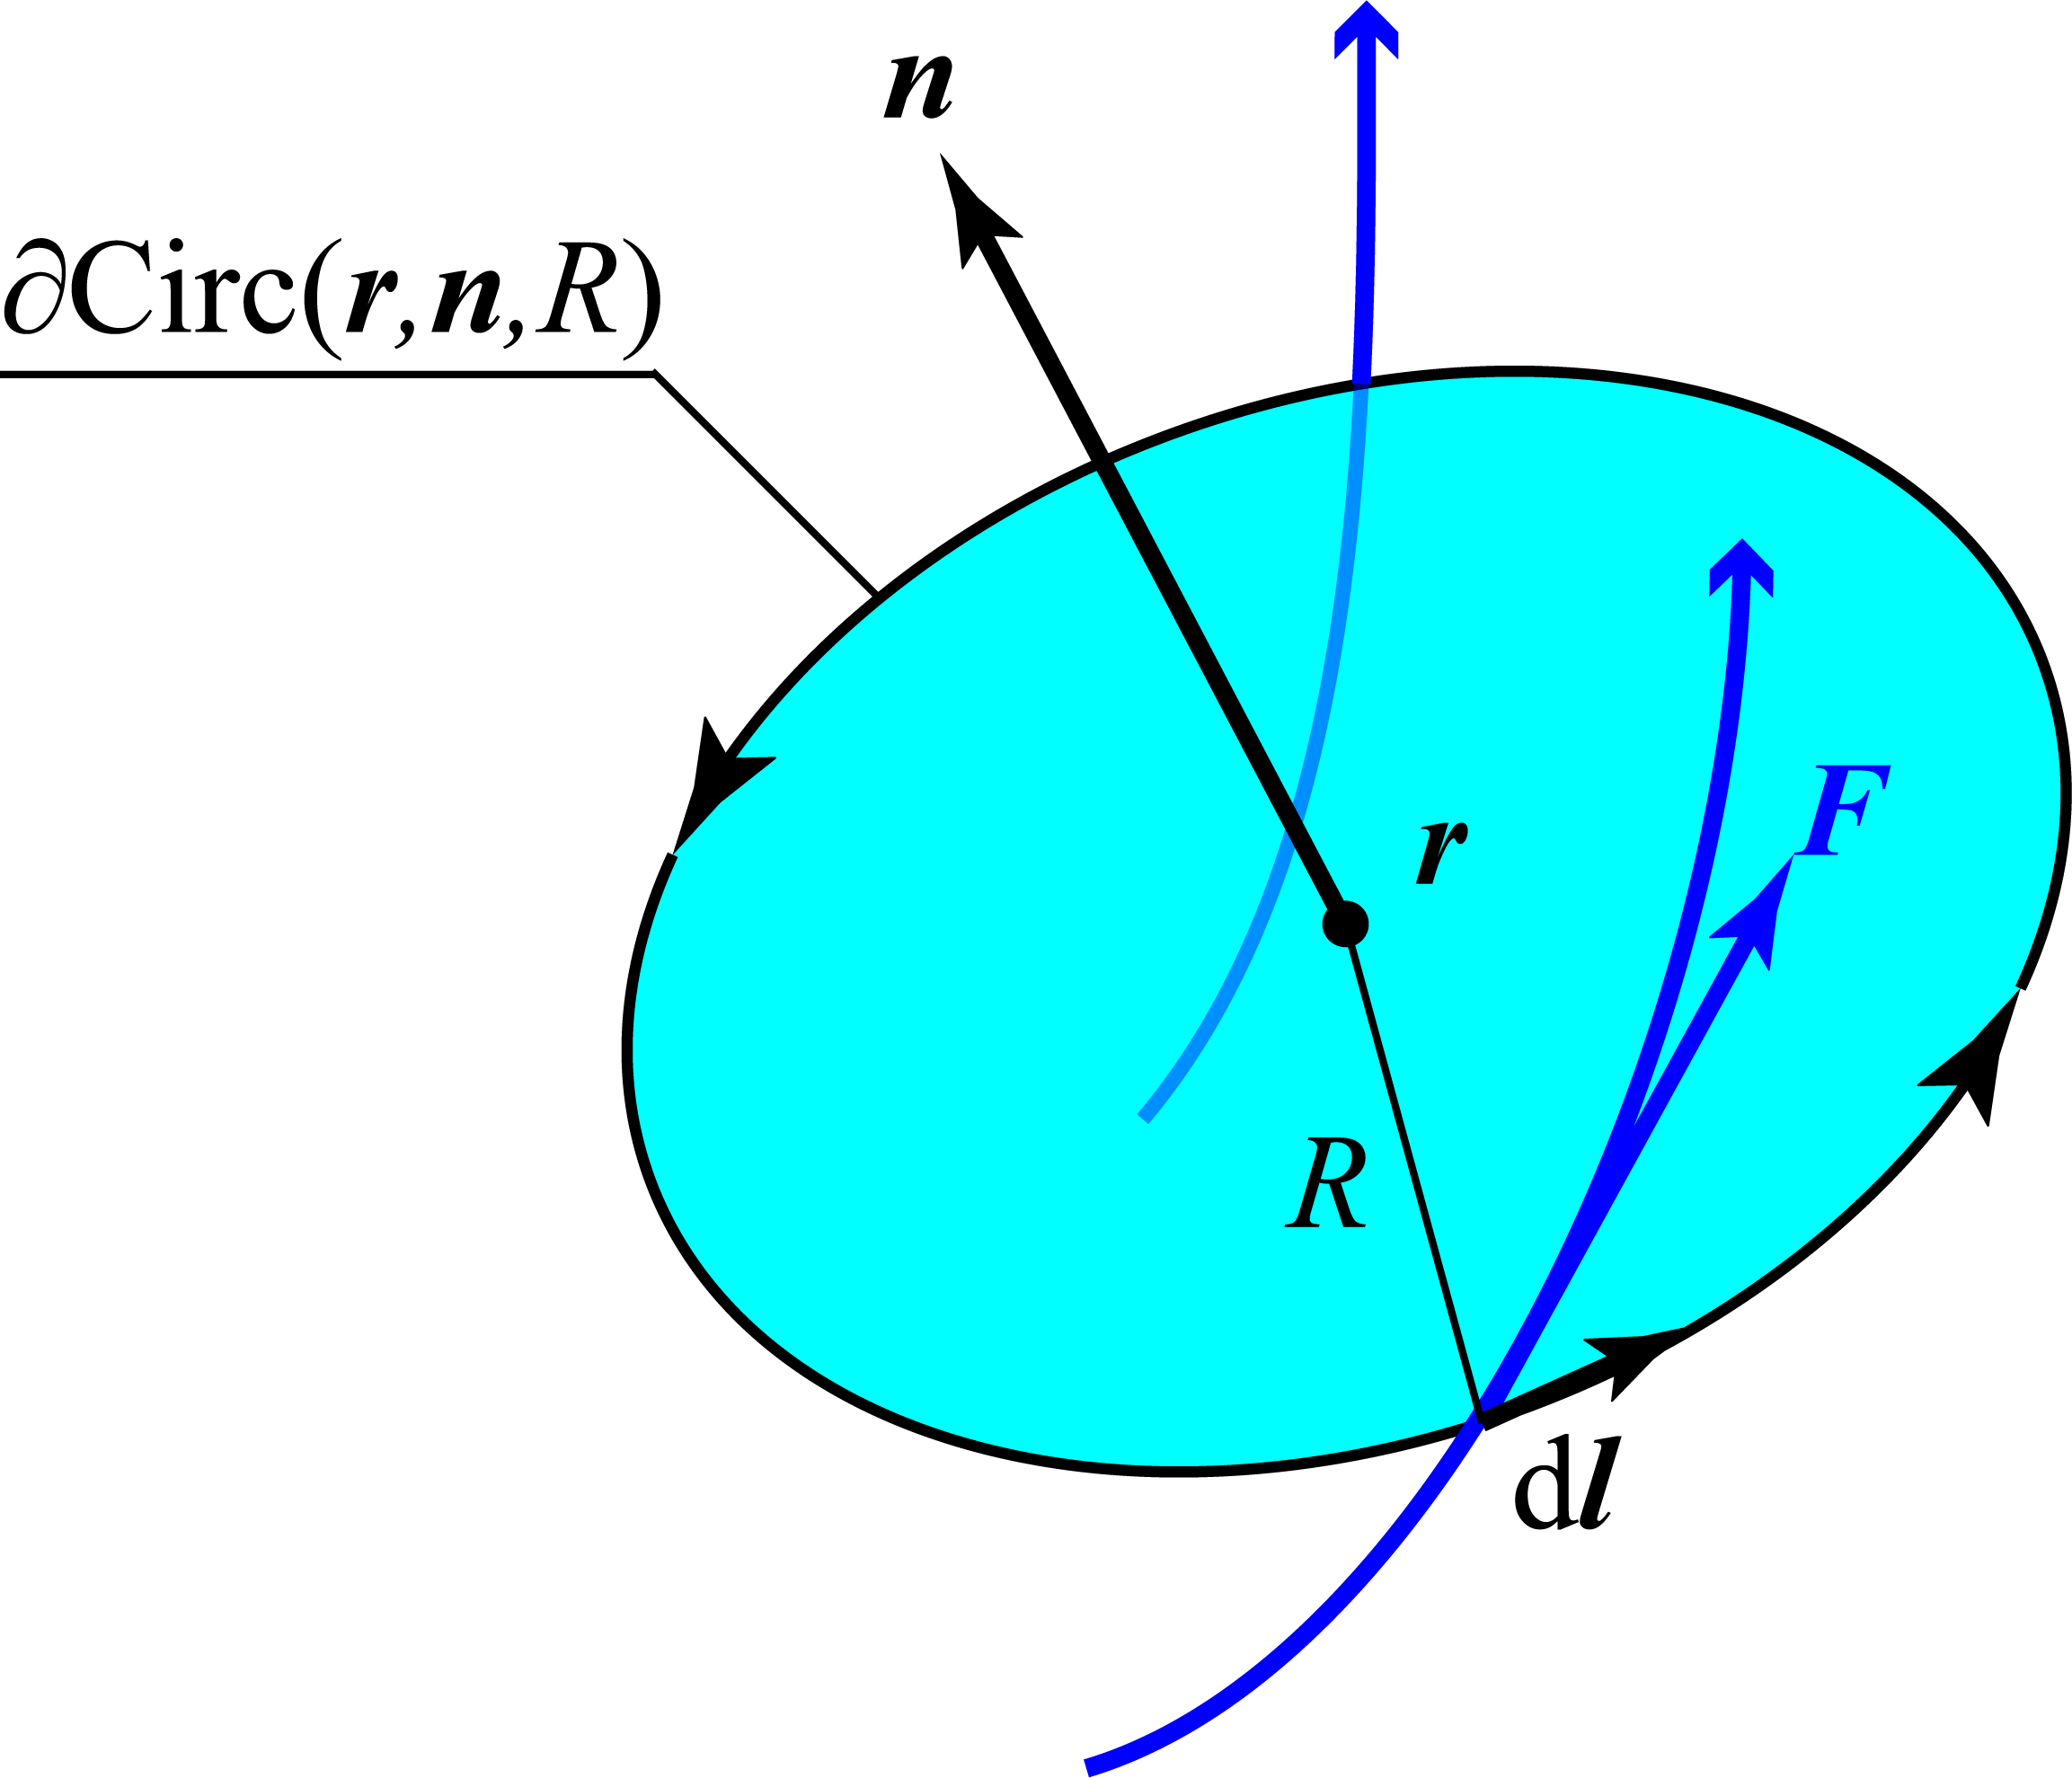
\includegraphics[width=7cm]{image/7-1-5.png}
\caption{矢量场的旋度}
\end{wrapfigure}
第二个概念便是\emph{旋度}(curl)了.\,它实际上代表矢量场的变化矩阵表中反对称的那一部分\footnote{任何一个矩阵都可以被唯一地分解为一个对称矩阵与反对称矩阵之和,\,前者有六个独立分量,\,包含原来的对角线与对称位置的两元素和的一半,\,后者仅有三个独立分量,\,为对称两个位置元素差的一半.}.\,它可以被写为一个矢量.\,与在这一点处的无限小的环积分有关,\,数学上不难证明:
\[\bs{n}\cdot\nabla\times \bs{F}=\lim_{R\to 0}\left.\left(\oint_{\partial {\rm Circ}(\bs{r},\bs{n},R)}\bs{F}\cdot \ud\bs{l}\right)\right/(\pi R^2)\]

由于半径为$R$的圆的选取还依赖于其朝向.\,故在上式中我们对积分的方向和垂直于积分圆面的法向单位矢量$n$采取了右手定则式的对应.\,而最后积分出来得到的数恰好是面法向单位矢量与从$\bs{F}$的各个导数中提取的旋度矢量的点乘.\,环积分通常被称为\emph{环量}(circulation),\,旋度则反应矢量场局域的涡旋程度.\,数学上可以证明旋度可以由行列式表示为:
\[\nabla\times \bs{F}=\begin{vmatrix}
\dfrac{\partial}{\partial x}&\dfrac{\partial}{\partial y}&\dfrac{\partial}{\partial z}\\
F_x&F_y&F_z\\
\bs{e}_x&\bs{e}_y&\bs{e}_z
\end{vmatrix}\]

作为与牛顿-莱布尼茨定理对应的散度与旋度版本,\,根据两个量的定义可知前者发生在体积内部的积分与其闭合表面上,\,后者发生在曲面上面积分和它的闭合曲线边界上:
\[\int\limits_V \nabla\cdot \bs{F}\ud V=\oint\limits_{\partial V}\bs{F}\cdot\ud\bs{A}\]
\[\int\limits_A \nabla\times \bs{F}\cdot\ud \bs{A}=\oint\limits_{\partial A}\bs{F}\cdot\ud\bs{l}\]

前者为\emph{奥斯特诺格拉德斯基-高斯定理}(Ostrogradsky-Gauss theorem),\,后者则为\emph{开尔文-斯托克斯定理}(Kelvin-Stokes theorem)\footnote{微分流形上的微分形式有一个\emph{嘉当-斯托克斯定理}(Cartan-Stokes theorem)统一了以上所有形式:
\[\oint\limits_{\partial \Omega}\omega=\int\limits_\Omega \ud \omega\]}.

现在让我们回到库仑定律,\,现在就必须把它理解为两个公式:
\[\bs{E}=\ke \frac{Q}{r^2}\bs{e}_r\quad ;\quad \bs{F}=q\bs{E}\]

前一半式子说明,\,即使没有引入任何试探电荷$q$,\,在空间中距离场源电荷$Q$为$r$处依然存在某种独立于电荷而存在的``场''.\,否则也就不可能对引入的电荷瞬间产生力的作用.\,这个场由电荷激发,\,以后将知道它有自己的能量与动量,\,而且都是可以被局域地确定\footnote{即,\,可以确定每一点的场能量动量密度.}.\,经典物理中似乎只能由电荷产生场,\,但高能物理下场也能反过来产生电荷粒子,\,实际上此时会将电磁场理解为``光子''这样的物质.\,电磁场的特点是能对带电荷的物质产生作用.

而后一半的式子则给出了电磁场中一点处电场强度矢量$\bs{E}$的定义.\,带电粒子如果在电磁场中静止,\,那么将受到一个与电荷量成正比的力.\,把力与电荷量的比值定义为电场强度矢量.

显然,\,带电粒子的引入也会产生电场.\,这个电场与原来场源电荷产生的电场叠加,\,形成了空间的真实电场分布.\,但在计算这个``试探电荷''的电场时,\,不应该考虑自己在自己这一点处产生的电场.\,因为自己对自己的力总是零.\,而总是计算``外场''在试探电荷这一点的值.\,不过,\,试探电荷的引入与否可能会对外界的场源电荷分部产生改变.\,从而改变外场.\,这又需要另说了,\,我们下一章的导体静电感应就是在不断讨论这个问题.

电场满足\emph{叠加原理}(superposition principle).\,我们总是一对一对地考虑电荷之间的二体作用,\,把相互作用力做非相干的矢量叠加.\,这也就是说,\,给定一个场源电荷分部,\,可以叠加计算出空间中任意一点的电场强度:
\[\bs{E}(\bs{r})=\int\limits_{V'} \ke \frac{\rho \bs{e}_{\bs{R}}}{\bs{R}^2} \ud V'\quad,\quad \bs{R}=\bs{r}-\bs{r}'\]
\[\bs{E}(\bs{r}):=\frac{\bs{F}_{\rm static}}{q}\]

也是出于这个原因,\,所有由电场强度派生出来的量:\,电势,\,电通量等等都符合线性的叠加原理.\,马上就会介绍,\,这是由于描述电场与电荷关系的基本方程是一个线性的微分方程的缘故.




\section{两个定律与电势}

库仑定律是静电学最基本的公理,\,但我们研究电场作为场的性质,\,它与电荷的关系.\,为以后深入了解电磁场整体打好基础.

\subsection{电场的高斯定律}

首先让我们研究\emph{电通量}(electric flux),\,通过一个曲面(不一定闭合)的电通量定义为曲面上电场强度的积分:
\[\varPhi=\int\limits_A \bs{E}\cdot\ud \bs{A}\]

我们在这儿必须引入有向曲线,\,曲面,\,体积的概念.\,固然,\,曲线,\,曲面,\,体积都没有方向与正负,\,它们仅仅是特定空间中的几何形状.\,但定义各种积分时,\,曲线积分的线元矢量$\ud\bs{l}$,\,曲面积分的面元矢量$\ud\bs{A}$都有两个可能的方向.\,而体积元$\ud V$也不一定恒正,\,在某些情况下将取负.\,那么我们通常会有一个符号约定:

\begin{enumerate}
	\item 对于\emph{可定向}(orientable)曲面(不可定向的比如莫比乌斯环),\,总是定义一个方向为正,\,即为每一个面元指定一个面元矢量,\,它取垂直于面的两个方向之一,\,而相邻的面元具有相同的取向.\,而如果涉及到面边界上闭合曲线的环积分,\,则线元矢量取的方向与面元构成\emph{右手定则}(right-hand rule).
	\item 对于\emph{连通}(connected)体积区域,\,如果取体积微元为正,\,那么涉及到区域边界闭合曲面上的面积分时,\,面元取从体积内到体积外的方向.\,如果取体积微元为负,\,则面上面元取体积外到体积内的方向.
\end{enumerate}

而我们之前写出的奥-高定理和开-斯定理,\,都是在这个意义下正确的.

从而以上电通量也就因为我们选择的面的两种可能的正向而造成两个不同的结果,\,它们相差一个相反数.

电场的\emph{高斯定律}(Gauss's law)指出:
\[\varPhi_{\partial V}=\oint\limits_{\partial V} \bs{E}\cdot\ud \bs{A}=\frac{1}{\varepsilon_0}\int\limits_V \rho\ud V\]

\begin{figure}[H]
\centering
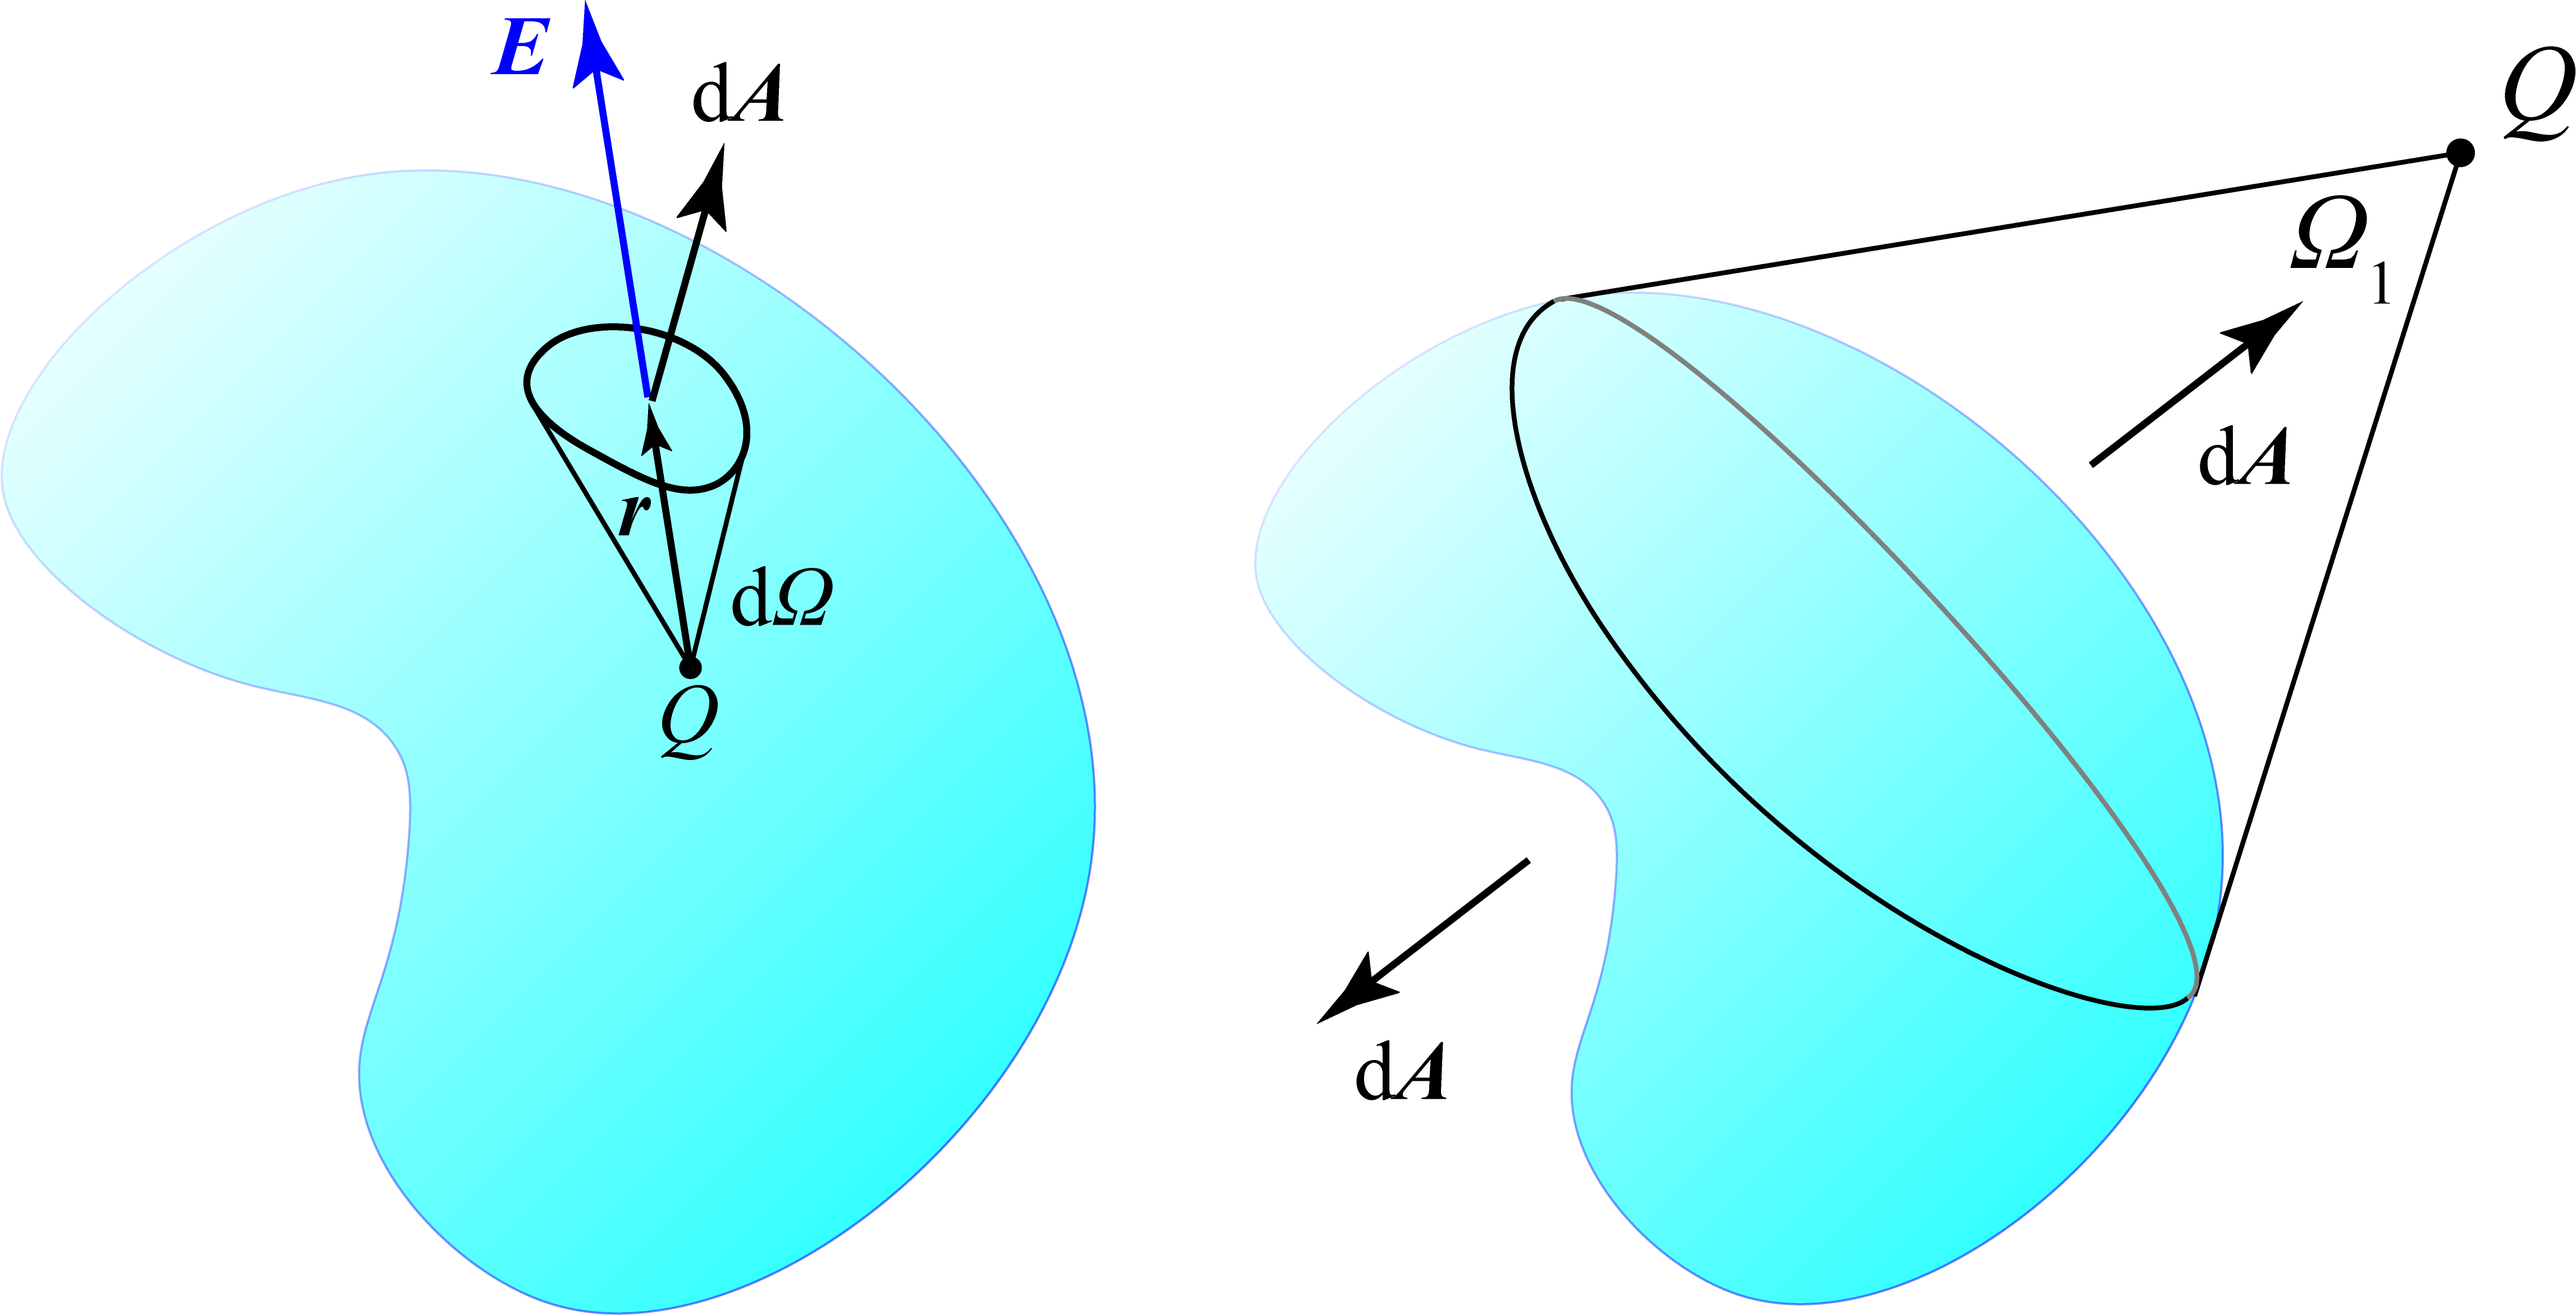
\includegraphics[width=0.5\textwidth]{image/7-1-6.png}
\caption{证明高斯定律}
\end{figure}

我们来用库仑定律证明高斯定律.\,首先考虑一个在闭合曲面内部的点电荷,\,我们发现面元上的通量:
\[\ud \varPhi=\bs{E}\cdot\ud \bs{A}=\ke \frac{Q\bs{e}_{\bs{r}}\cdot\ud \bs{A}}{\bs{r}^2}\]

而这一个小面元对点电荷张的立体角恰好是:
\[\ud\varOmega=\frac{\bs{e}_{\bs{r}}\cdot\ud \bs{A}}{\bs{r}^2}\]

故对面积分总立体角给出$4\pi$的结果:
\[\ud \varPhi=\frac{Q}{\varepsilon_0}\cdot\frac{\ud\varOmega}{4\pi}\quad \Rightarrow\quad \varPhi=\frac{Q}{\varepsilon_0}\cdot\oint\limits_{\partial V}\frac{\ud\varOmega}{4\pi}=\frac{Q}{\varepsilon_0}\]

我们再考虑在面外的点电荷$Q$对面产生的电通量,\,此时面的正向与点电荷产生电场方向的点乘就有了正负号,\,积分以后得到的结果是通过点电荷去看曲面,\,把曲面对点电荷张的最大视角处的曲线找到,\,将曲面分为两个部分,\,立体角都是$\varOmega_1$,\,总积分为:
\[\varPhi=\frac{Q}{\varepsilon_0}\cdot\oint\limits_{\partial V}\frac{\ud\varOmega}{4\pi}=\frac{Q}{\varepsilon_0}(\varOmega_1-\varOmega_1)=0\]

从而我们证明了,\,电荷若在闭合曲面内,\,则电通量贡献为\(\frac{Q}{\varepsilon_0}\).\,而若在闭合曲面外,\,则电通量贡献为$0$.\,再由叠加原理,\,得任意情况下闭合曲面的电通量等于内部总电荷量除真空介电常数$\varepsilon_0$.\,考虑电荷连续分布或准连续分布的情况下,\,有:
\[\oint\limits_{\partial V} \bs{E}\cdot\ud \bs{A}=\frac{1}{\varepsilon_0}\int\limits_V \rho\ud V\]

此即高斯定律,\,由数学上的奥-高定理,\,我们可以把上式写为局域的微分形式:
\[\nabla\cdot\bs{E}=\frac{\rho}{\varepsilon_0}\]

高斯定律旨在说明:\,电荷产生电场(电荷是电场的源强度).

\subsection{电势与电场的环路定律}

对点电荷产生的电场$\bs{E}=\dfrac{Q}{4\pi\varepsilon_0 r^2}\bs{e}_r$,\,再引入以下标量场是方便的:
\[\varphi=\ke\frac{Q}{r}\]

这是因为如果计算球坐标下的梯度:
\[\nabla=\bs{e}_r\frac{\partial}{\partial r}+\frac{\bs{e}_\theta}{r}\frac{\partial}{\partial \theta}+\frac{\bs{e}_\varphi}{r\sin\theta}\frac{\partial}{\partial \varphi}\]

便得到以下关系式:
\[\bs{E}=-\nabla\varphi\]

即电场可以表示为我们引入的另一个标量场的负梯度的形式.\,这个标量场就叫做\emph{电势}(electric petential).\,而以上关系,\,结合梯度的含义理解,\,便是沿电场线方向电势降低.\,可以通过牛-莱定理写为积分形式(下式与路径无关):
\[\int_A^B \bs{E}\cdot \ud\bs{l}=\varphi_A-\varphi_B\]

以上关系式由叠加原理,\,在任意电荷分部的情况下都成立,\,此时对应的电势标量场为:
\[\varphi(\bs{r})=\int \ke\frac{\rho}{|\bs{R}|}\ud V'\quad ,\quad \bs{R}=\bs{r}-\bs{r}'\]

对于电势的引入可能存在一点疑惑:\,我们都知道电场的定义是可以独立于场源电荷的,\,它为在一点处引入静止的试探电荷时单位电荷的受力.\,那么电势是否可以独立于场源电荷而定义呢?\,观点一比较基础,\,它认为在静电场情况下既然全空间电场已经被定义了,\,它就应该反映了该点处场的全部实际信息,\,那么电势作为与电场符合一个梯度关系的梯度场,\,也就能被相应的确定下来,\,两个可能的电势还可以差一个全空间都一致的常数.\,也就是这种观点把电场视为更加基础的场的特征.\,下面便可以知道电势的含义是引入试探电荷后单位试探电荷在该点处的电势能.\,而观点二则更加本质,\,我们今天知道了势比场强实际上包含更多的信息.\,由于微观粒子的量子特性,\,力的概念已然失效,\,从而场强反而不如用势来描述一个场更为直接而实用.\,电磁场论实际上也就是一个是矢量场论,\,它由矢势和标势组成一个四维矢量来完整地描述,\,但取法不唯一,\,多出来的冗余自由度被称为\emph{规范}(gauge),\,它恰好就在表示电荷与场的相互作用时,\,与电荷的量子相位协同变化,\,从而造成实际可以观测的影响.\,为了实际问题的方便,\,通常约定势有特定的取法.\,在静电学的常见情况下(电荷分布区域有限时),\,常常取无穷远处电势为零,\,注意上电势积分式也恰恰符合这一点.

我们进一步考察电势的物理含义,\,如果把以上电场视为外电场,\,引入试探电荷$q$,\,并在以上积分形式的场强与势的关系中乘以$q$,\,便发现$q\bs{E}$就是电荷的受力,\,左边就是表示电场力的做功:
\[W_{A\to B}=q\varphi_A-q\varphi_B\]

很自然地我们发现电场力是保守力,\,而对应的电势能,\,基于它应该与电荷量成正比的观点,\,我们总是直接取为:
\[E_p=q\varphi\]

从而电势的效果,\,是为试探电荷带来一个电势能.

最后我们再考察电场的一个特性,\,由于任何路径上的电场积分可以根据牛-莱定理写为端点的电势差的形式,\,考虑闭合的曲线积分,\,它可以看成一个可定向曲面的边界,\,由于两端点重合:
\[\oint\limits_{\partial A}\bs{E}\cdot\ud \bs{l}=0\]

这就是电场的\emph{环路定律}(circuital law),\,再根据数学上的开-斯定理,\,我们写出环路定律的微分形式:
\[\nabla\times\bs{E}=\bs{0}\]

也就是静电场无旋.\,值得指出这不过是静电场可以表示为标量电势场的负梯度的直接结果,\,因为任意一个标量场的梯度都是无旋的\footnote{这个结论向流形推广就是著名的\emph{庞加莱引例}(Poincar'e lemma)了,\,它指出任意$p-$形式$\omega$的二次全微分为零:
\[\ud\ud\omega=0\]

一个以后会用得上的推论可以通过考察矢量场的旋度在闭合曲面上的面积分,\,而把闭合曲面看成是边界曲线缩小到零的有边界曲面而得:
\[\oint\limits_{\partial V}\nabla \times \bs{F}\cdot\ud \bs{A}=0\quad \Rightarrow \quad \nabla\cdot\nabla \times\bs{F}=0\]}:
\[\oint\limits_{\partial A}\nabla f\cdot\ud \bs{l}=0\quad \Rightarrow \quad \nabla\times\nabla f=\bs{0}\]

\subsection{总结}

\begin{wrapfigure}[9]{o}[0pt]{8cm}
\centering
\vspace{-0.1cm}
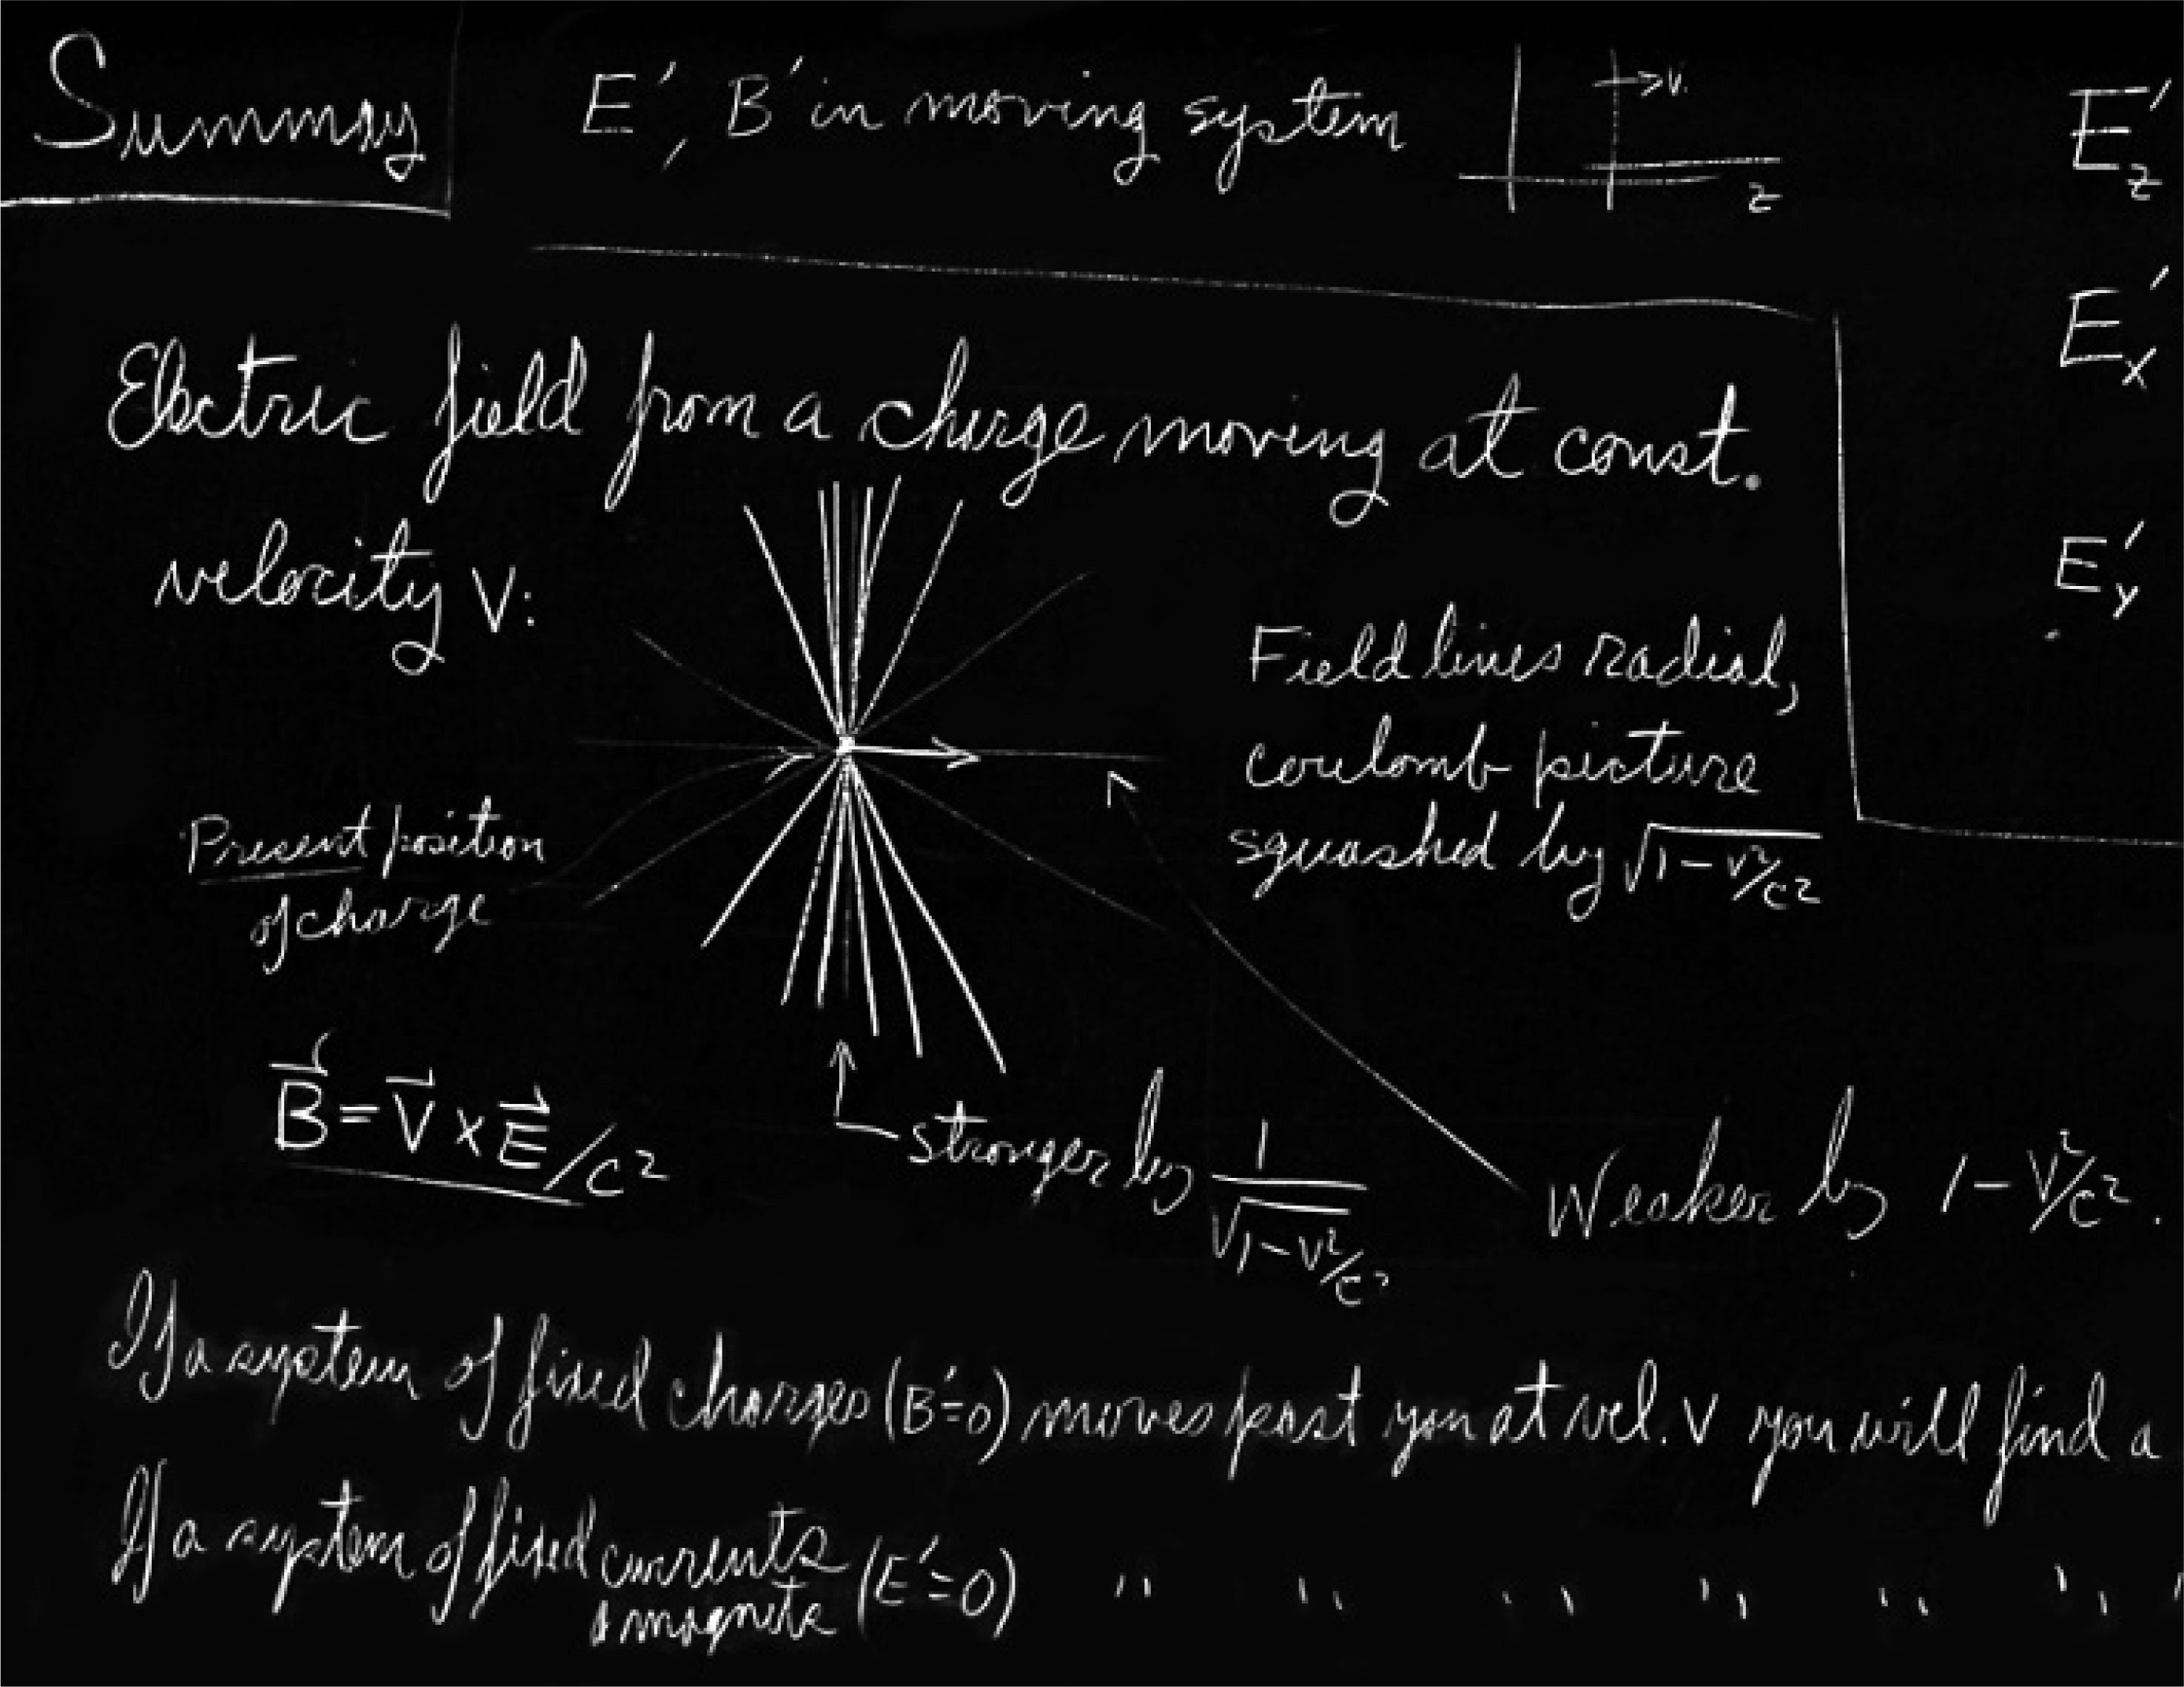
\includegraphics[width=8cm]{image/7-1-7.png}
\caption{Feynman讲座一瞥}
\end{wrapfigure}
我们现在有三个不同的层次去看待电荷与电荷之间的相互作用问题\footnote{拉普拉斯算子$\nabla^2=\nabla\cdot\nabla$,\,如作用在标量上即表示先求梯度后求散度:
	\[\nabla^2f=\nabla\cdot(\nabla f)\]}:
\begin{description}
	\item[{\hei 1. 不引入场:}]

	\[\bs{F}=\ke\frac{Qq}{r^2}\bs{e}\]

	\item[{\hei 2. 引入场,\,用场强描述:}]

	\[\nabla\cdot \bs{E}=\frac{\rho}{\varepsilon_0}\quad ;\quad \nabla\times\bs{E}=\bs{0}\]
	\[\bs{F}=q\bs{E}\]

	\item[{\hei 3. 引入场,\,用势描述:}]
	\[\nabla^2 \varphi=-\frac{\rho}{\varepsilon_0}\]
	\[E_p=q\varphi\]
\end{description}


以上描述一个比一个适用范围更广,\,第一个仅仅适用于静电场或低速情况,\,第二个则是对高速运动的电荷与电磁场适用,\,比如匀速运动的电荷的场强由简单相对论讨论可得:
\[\bs{E}=\ke\frac{Q}{r^2}\frac{1-\beta^2}{(1-\beta^2\sin^2\theta)^{3/2}}\bs{e}_r\]
\[\bs{B}=\frac{\bs{v}\times\bs{E}}{c^2}\]

它要符合第二个式子(旋度需要做相对论修正),\,而第三个式子更是适用于非经典场论情况.


\section{静电能}

我们将进一步深入研究电场相互作用中的能量概念.

\subsection{静电势能}

\begin{wrapfigure}[13]{o}[0pt]{8cm}
\centering
\vspace{-0.1cm}
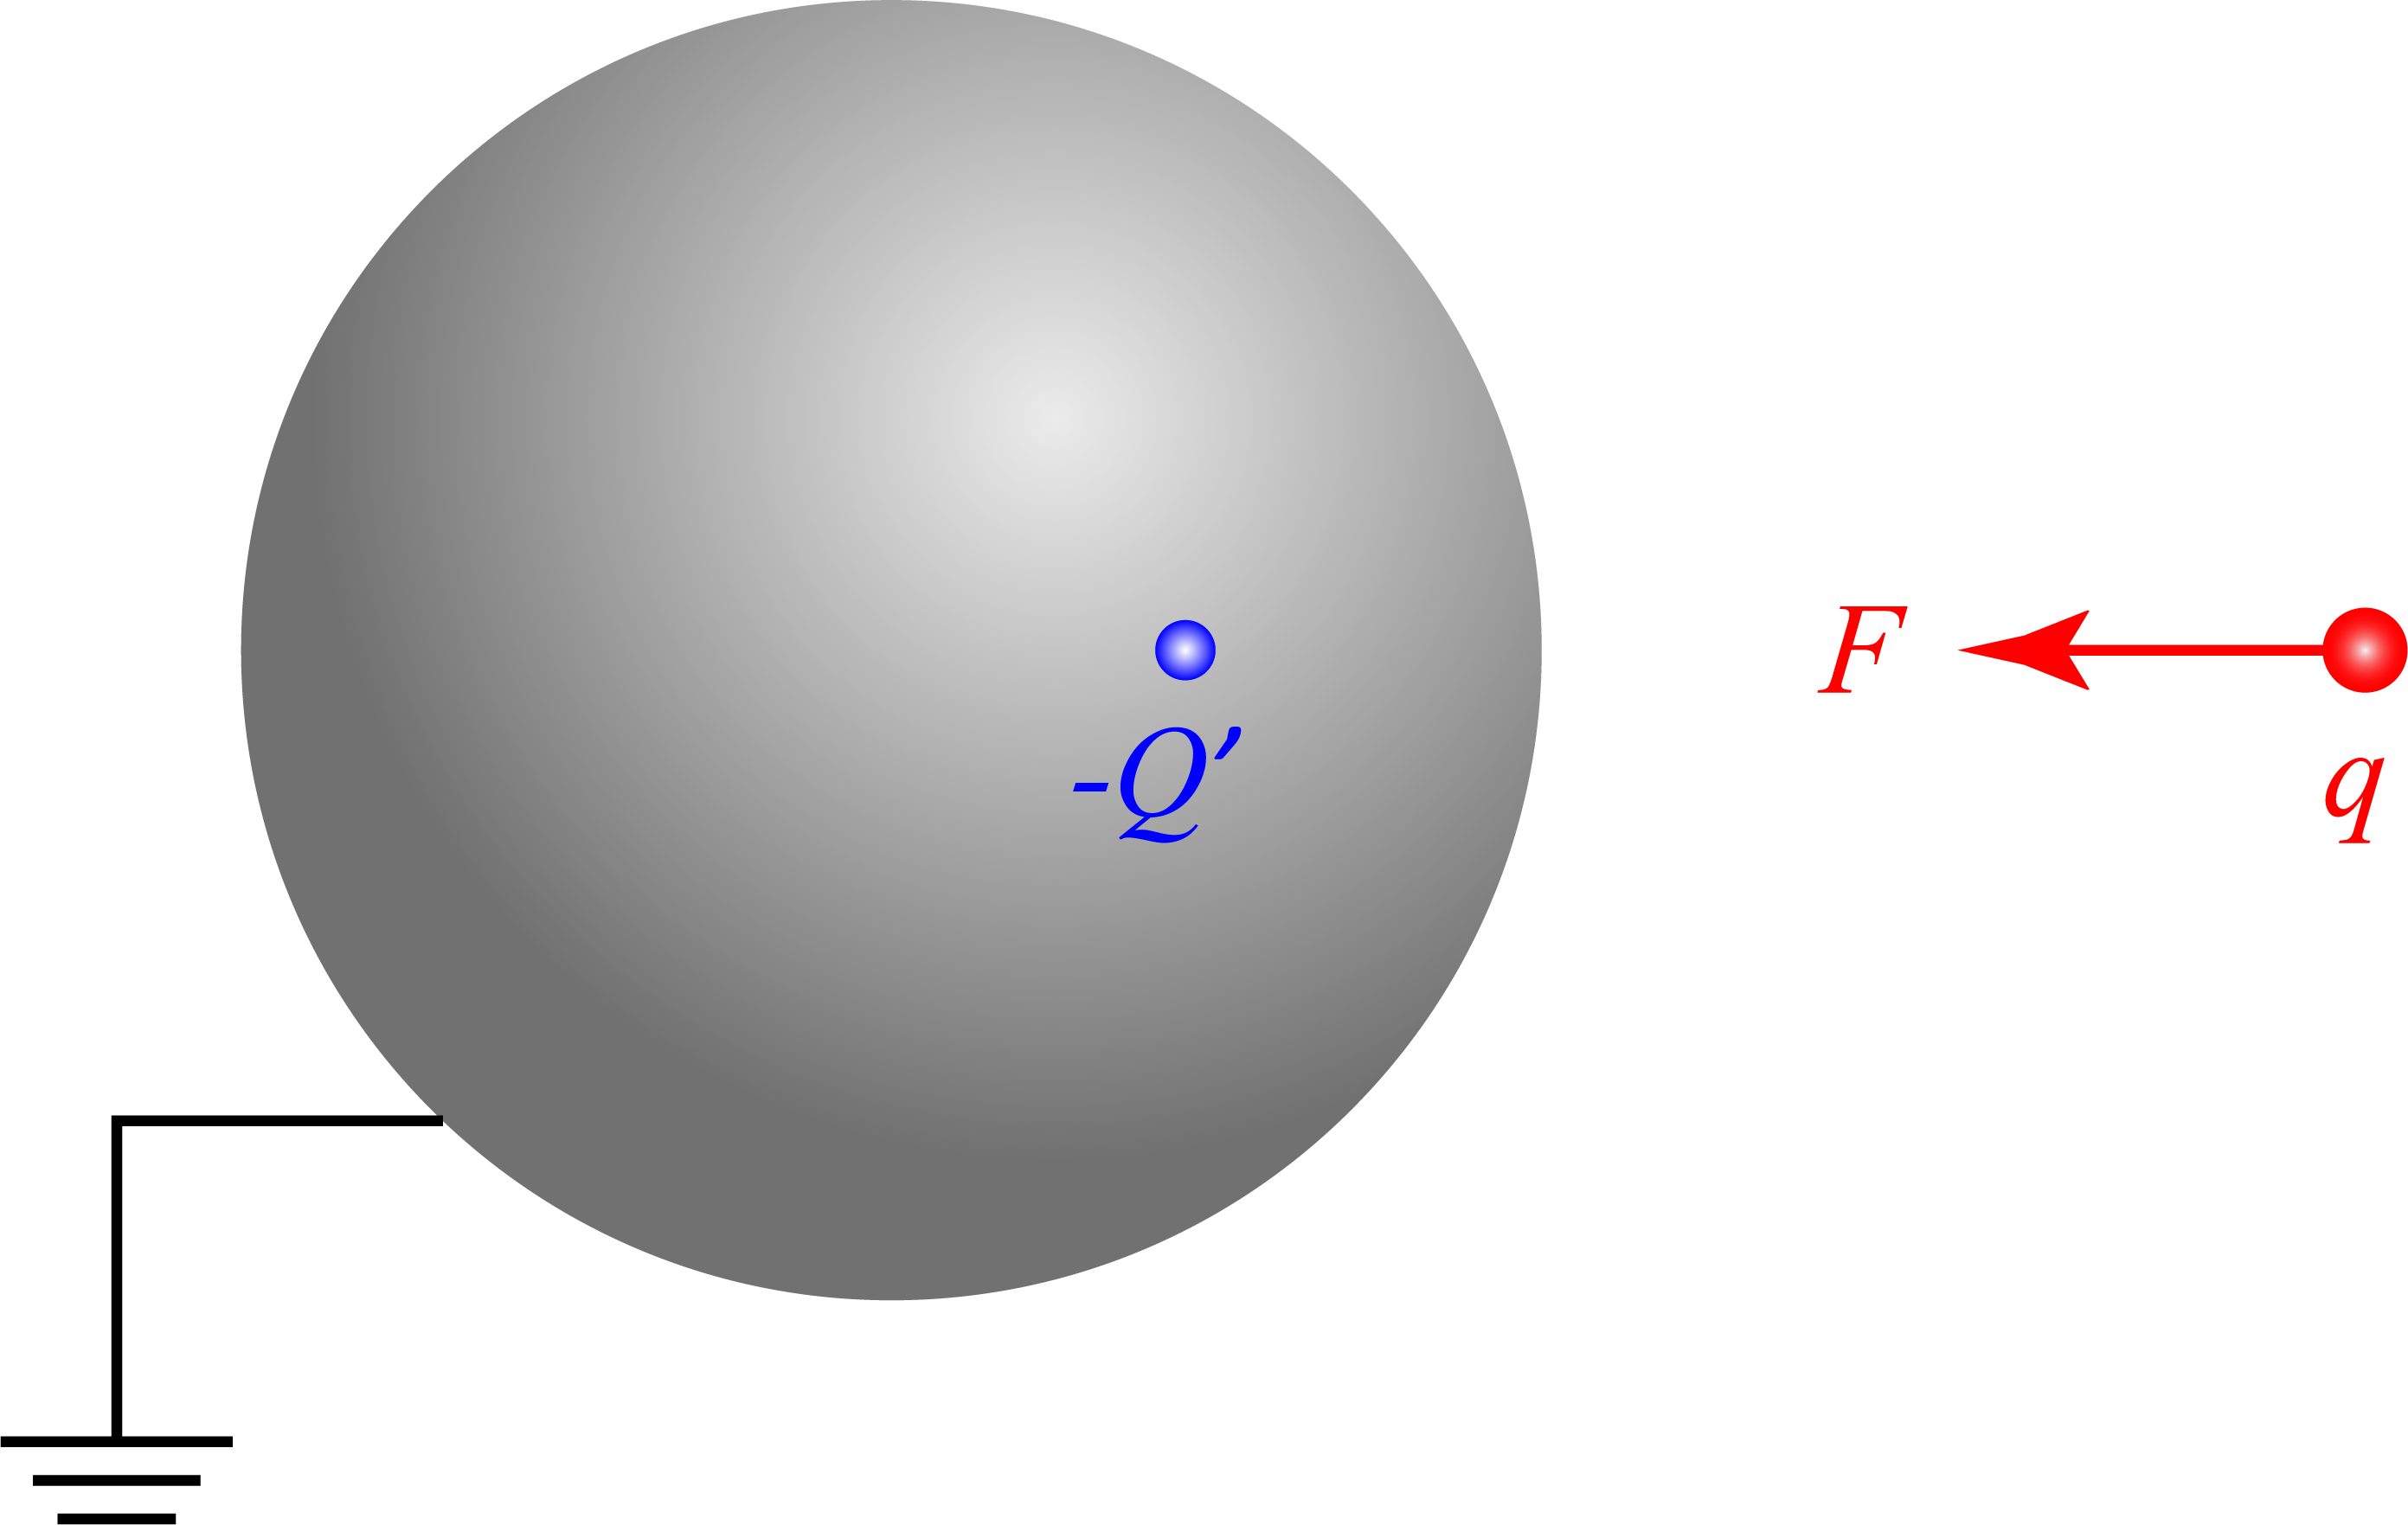
\includegraphics[width=8cm]{image/7-1-8.png}
\caption{情形:\,场源电荷取决于试探电荷}
\end{wrapfigure}
之前已经引入了电势能的概念,\,我们把外场中引入的试探电荷(点电荷)所具有的势能的大小计做电势能,\,并得出了电势能的表达式:
\[E_p=q\varphi\]

还指出了,\,它的作用是用来表示不变的外电场对电荷的做功的多少,\,基于这样的观察,\,我们把这个能量称为\emph{静电势能}(electrostatic potential energy),\,静电的含义,\,是要求外场不能随着试探电荷的引入与移动而改变.\,而更常见的一类情况是,\,随着试探电荷的移动,\,场源电荷也在随着改变,\,如之后将会经常讨论的静电感应的情况.\,此时仍然可以计算外场的场强与电势,\,并引入试探电荷以后依然可以形式地写出\emph{电势能}(electro potential energy)的值$E_p=q\varphi$,\,但它不再代表实际移动试探电荷电场对电荷做的功了,\,它代表什么?\,电场对电荷做功普遍地应该怎么表示?\,外力做功又如何和它发生联系,\,这是我们之后的讨论关心的问题.

首先对于这个问题的第一步考察是,\,虽然试探电荷的特定位置带来特定的外场,\,但一旦确定了外场的场源的电荷分布,\,便可以独立于试探电荷地产生一个分布于全空间的电势与电场,\,而可以设想固定这个电荷分布不变,\,而把试探电荷放在空间中的任意一点,\,讨论其受力与能量.\,这些改变试探电荷位置而不改变外场的位移称为\emph{虚位移}(virtual displacement).\,它是一种广泛用来建立理论模型的方法.\,它的强大之处在于虚位移的任意性,\,在每一个实际时刻试探电荷可以在任意位置,\,外场在缓慢随时间发生改变,\,而试探电荷发生的实际位移是所有虚位移中的一个特例.\,在这个意义下,\,电势能的含义便在于,\,试探电荷发生虚位移时,\,即场源电荷分布不变时,\,电场力对试探电荷做的虚功即为电势能的减小,\,此即静电场下的虚功原理:
\[\delta E_p=-q\bs{E}\cdot\delta \bs{r}\]

我们可以把这个概念推广,\,如果在该外场中引入不止一个点试探电荷,\,我们写出一个电荷体系在外场中的电势能来:
\[E_p=\sum_i q_i\varphi_i\]

这个写法存在一些问题,\,首先是如果没有引入任何试探电荷,\,体系是否固有一个能量?\,用场的角度来理解就会发现不对,\,场是一种物质,\,物质必定伴随着能量.\,或者考虑场源电荷之间的相互作用,\,它也一定会伴随着能量.\,再者,\,引入两个以上的点电荷时,\,它们之间的相互作用能没有被包含在以上项中.\,第三,\,即使是单个点电荷单独存在,\,也必定会带来其自能.\,我们需要从更基础的角度来讨论电荷体系的能量.




\subsection{自能与相互作用能}

考虑真空中的两个点电荷之间的相互作用.\,电荷$q_1$在电荷$q_2$处产生的电场与电势为$\bs{E}_{12}$与$\varphi_{12}$,\,电荷$q_2$在电荷$q_1$处产生的电场与电势为$\bs{E}_{21}$与$\varphi_{21}$无疑,\,相互作用力是相互的,\,满足牛顿第三定律$q_1\bs{E}_{21}+q_2\bs{E}_{12}=\bs{0}$.\,那么电势能是相互的吗?\,注意到:
\[q_1U_{21}=\ke\frac{q_1q_2}{r}=q_2U_{12}\]

从而两个电势能实际上是相等的.\,根据电势能的定义,\,它等于$1$不动$2$移到无穷远电场力所做的功,\,也会等于$2$不动$1$移到无穷远电场力所做的功.\,这两种情况平移对称,\,从而我们有理由判断:\,无论如何移动两个电荷,\,将$1$与$2$分开到无限远时电场力做功都会是以上值,\,这一点也不难在数学上证明.

从而我们把这个能量称为$12$间相互作用力对应的\emph{相互作用能}(interaction energy).\,它可以用任何一个电荷乘以另一个电荷在这个电荷处产生的势相乘得到,\,或者找到这一对相互作用,\,直接写出:
\[I_{12}=\ke\frac{q_1q_2}{r_{12}}\]

按照这思路,\,由叠加原理,\,我们可以很轻易地写出点电荷体系与连续分布电荷体系的总相互作用能:
\begin{description}
	\item[{\hei 1. 点电荷体系:}]
	\[I=\sum_{\{i,j\}!} \ke\frac{q_iq_j}{r_{ij}}\]
	\item[{\hei 2. 连续分布电荷体系:}]
	\[I= \iint\limits_{\{\ud V,\ud V'\}!}\ke\frac{\rho\rho'}{r}\ud V\ud V'\]
\end{description}

关于以上求和我们做出以下解释:

首先,\,点电荷体系的相互作用能表示把点电荷从计算这个能量的状态移动到点电荷彼此之间都相距无穷远时电场力所做的功.\,但一定要注意每个点电荷移动到无穷远以后还会因为自身的电磁相互作用而产生一个待定的能量,\,叫做自能,\,我们紧接着会讨论到这个问题.\,而连续分布电荷体系则表示把每一份电荷微元移动到无穷远以后电场力做的功,\,移动到无穷远以后电荷无限分散(宏观意义上),\,所以每一份微元电荷对应的电磁相互作用能真实地趋于零,\,故我们计算的这个能量就是这个体系的总电磁相互作用对应的能量.

第二,\,是这个求和表示的含义.\,我们用$(i,j)$来表示特定集合中两个元素$i,j$构成的\emph{有序对}(ordered pair),\,而$\{i,j\}$则表示交换$i,j$后表示同一代数元素的\footnote{以后还会用到$n$个元素的\emph{对称无序类}(symmetrized unordered setoid)与\emph{反对称无序类}(antisymmetrized unordered setoid):
\[\{i_1\cdots i_p\cdots i_q\cdots i_n\}=\{i_1\cdots i_q\cdots i_p\cdots i_n\}\]
\[[i_1\cdots i_p\cdots i_q\cdots i_n]=-[i_1\cdots i_q\cdots i_p\cdots i_n]\]
}\emph{对称无序对}(symmetrized unordered pair),\,即$\{i,j\}=\{j,i\}$.\,求和下加这个对符号表示对所有一对一对的情况进行求和.\,每一对只需要求一次即可.\,这之后还跟着一个感叹号,\,它表示$i,j$必须取不同值(而$\ud V$与$\ud V'$可以取相同值,\,这些项会在体积很小时求和也很小而可以忽略).\,那么由简单的代数变形,\,我们发现上两式即:
\[I=\frac{1}{2}\sum_i\sum_{j\neq i}\ke\frac{q_iq_j}{r_{ij}}=\frac{1}{2}\sum_iq_i\phi_i\]
\[I=\frac{1}{2}\int\limits_{\ud V}\int\limits_{\ud V'}\ke\frac{\rho\rho'}{r}\ud V\ud V'=\frac{1}{2}\int\limits_{\ud V}\rho \varphi \ud V\]

注意到第一式中$\phi_i$表示的是别的电荷在$q_i$处产生的电势,\,不包括自己在自己上产生的,\,我们把符号稍微变动一下以示区别.\,而在后一个表达式中则不需要考虑这种区别,\,这个式子将作为一个普遍的求总电磁相互作用能的表达式而使用.

第三,\,是这个求和的使用方法.\,实际上,\,如果电荷连续分布系统从一个状态变化到另一个状态,\,电荷分布与它产生的电势分布都发生改变,\,那么前后的能量增加:
\[\Delta I=\frac{1}{2}\int\rho' \varphi' \ud V-\frac{1}{2}\int\rho \varphi \ud V\]

自然表示电场对电荷体系所做的负功,\,或者表示由电荷流向电场的能量,\,它使得场的能量,\,也就是$I$,\,发生了增长\footnote{场只能和带荷的物质发生作用,\,这也是唯一的使得场能量变化的方法}.\,而反过来考察电荷体系,\,如果外力对电荷体系做功为$W$,\,那么根据动能定理应该有:
\[W-\Delta I=\Delta E_k\]

在十分缓慢地移动电荷的情况下,\,亦或是导体在载流子为电子,\,其动能十分的小可以忽略的情况下,\,动能的增长可以视为零,\,从而有:
\[W=\Delta I\]

即,\,外力做功,\,通过电荷为媒介,\,转化为了场的能量的增长.\,这个观点也是我们经常用的到的.

我们最后回到电势能与相互作用能的关系,\,考虑整个体系由两部分电荷体系构成,\,那么由叠加原理,\,整个空间中每一点的电势可以写成两部分贡献的和$\varphi_1+\varphi_2$.\,我们只需要对全空间的电荷积分,\,就得到了整个体系的相互作用能:
\begin{align*}
I 	&=\frac{1}{2}\int\limits_{\rm I+II}\rho \varphi \ud V \\
	&=\frac{1}{2}\int\limits_{\rm I}\rho_1 (\varphi_1+\varphi_2)\ud V_1 + \frac{1}{2}\int\limits_{\rm II}\rho_2 (\varphi_1+\varphi_2)\ud V_2 \\
	&=\frac{1}{2}\int\limits_{\rm I}\rho_1 \varphi_1\ud V_1+\frac{1}{2}\int\limits_{\rm II}\rho_2 \varphi_2\ud V_2+\frac{1}{2}\left(\int\limits_{\rm I}\rho_1 \varphi_2\ud V_1+\int\limits_{\rm II}\rho_2 \varphi_1\ud V_2\right) \\
	&=I_1+I_2+I_{12}
\end{align*}

\begin{wrapfigure}[14]{o}[0pt]{9cm}
\centering
\vspace{-0.1cm}
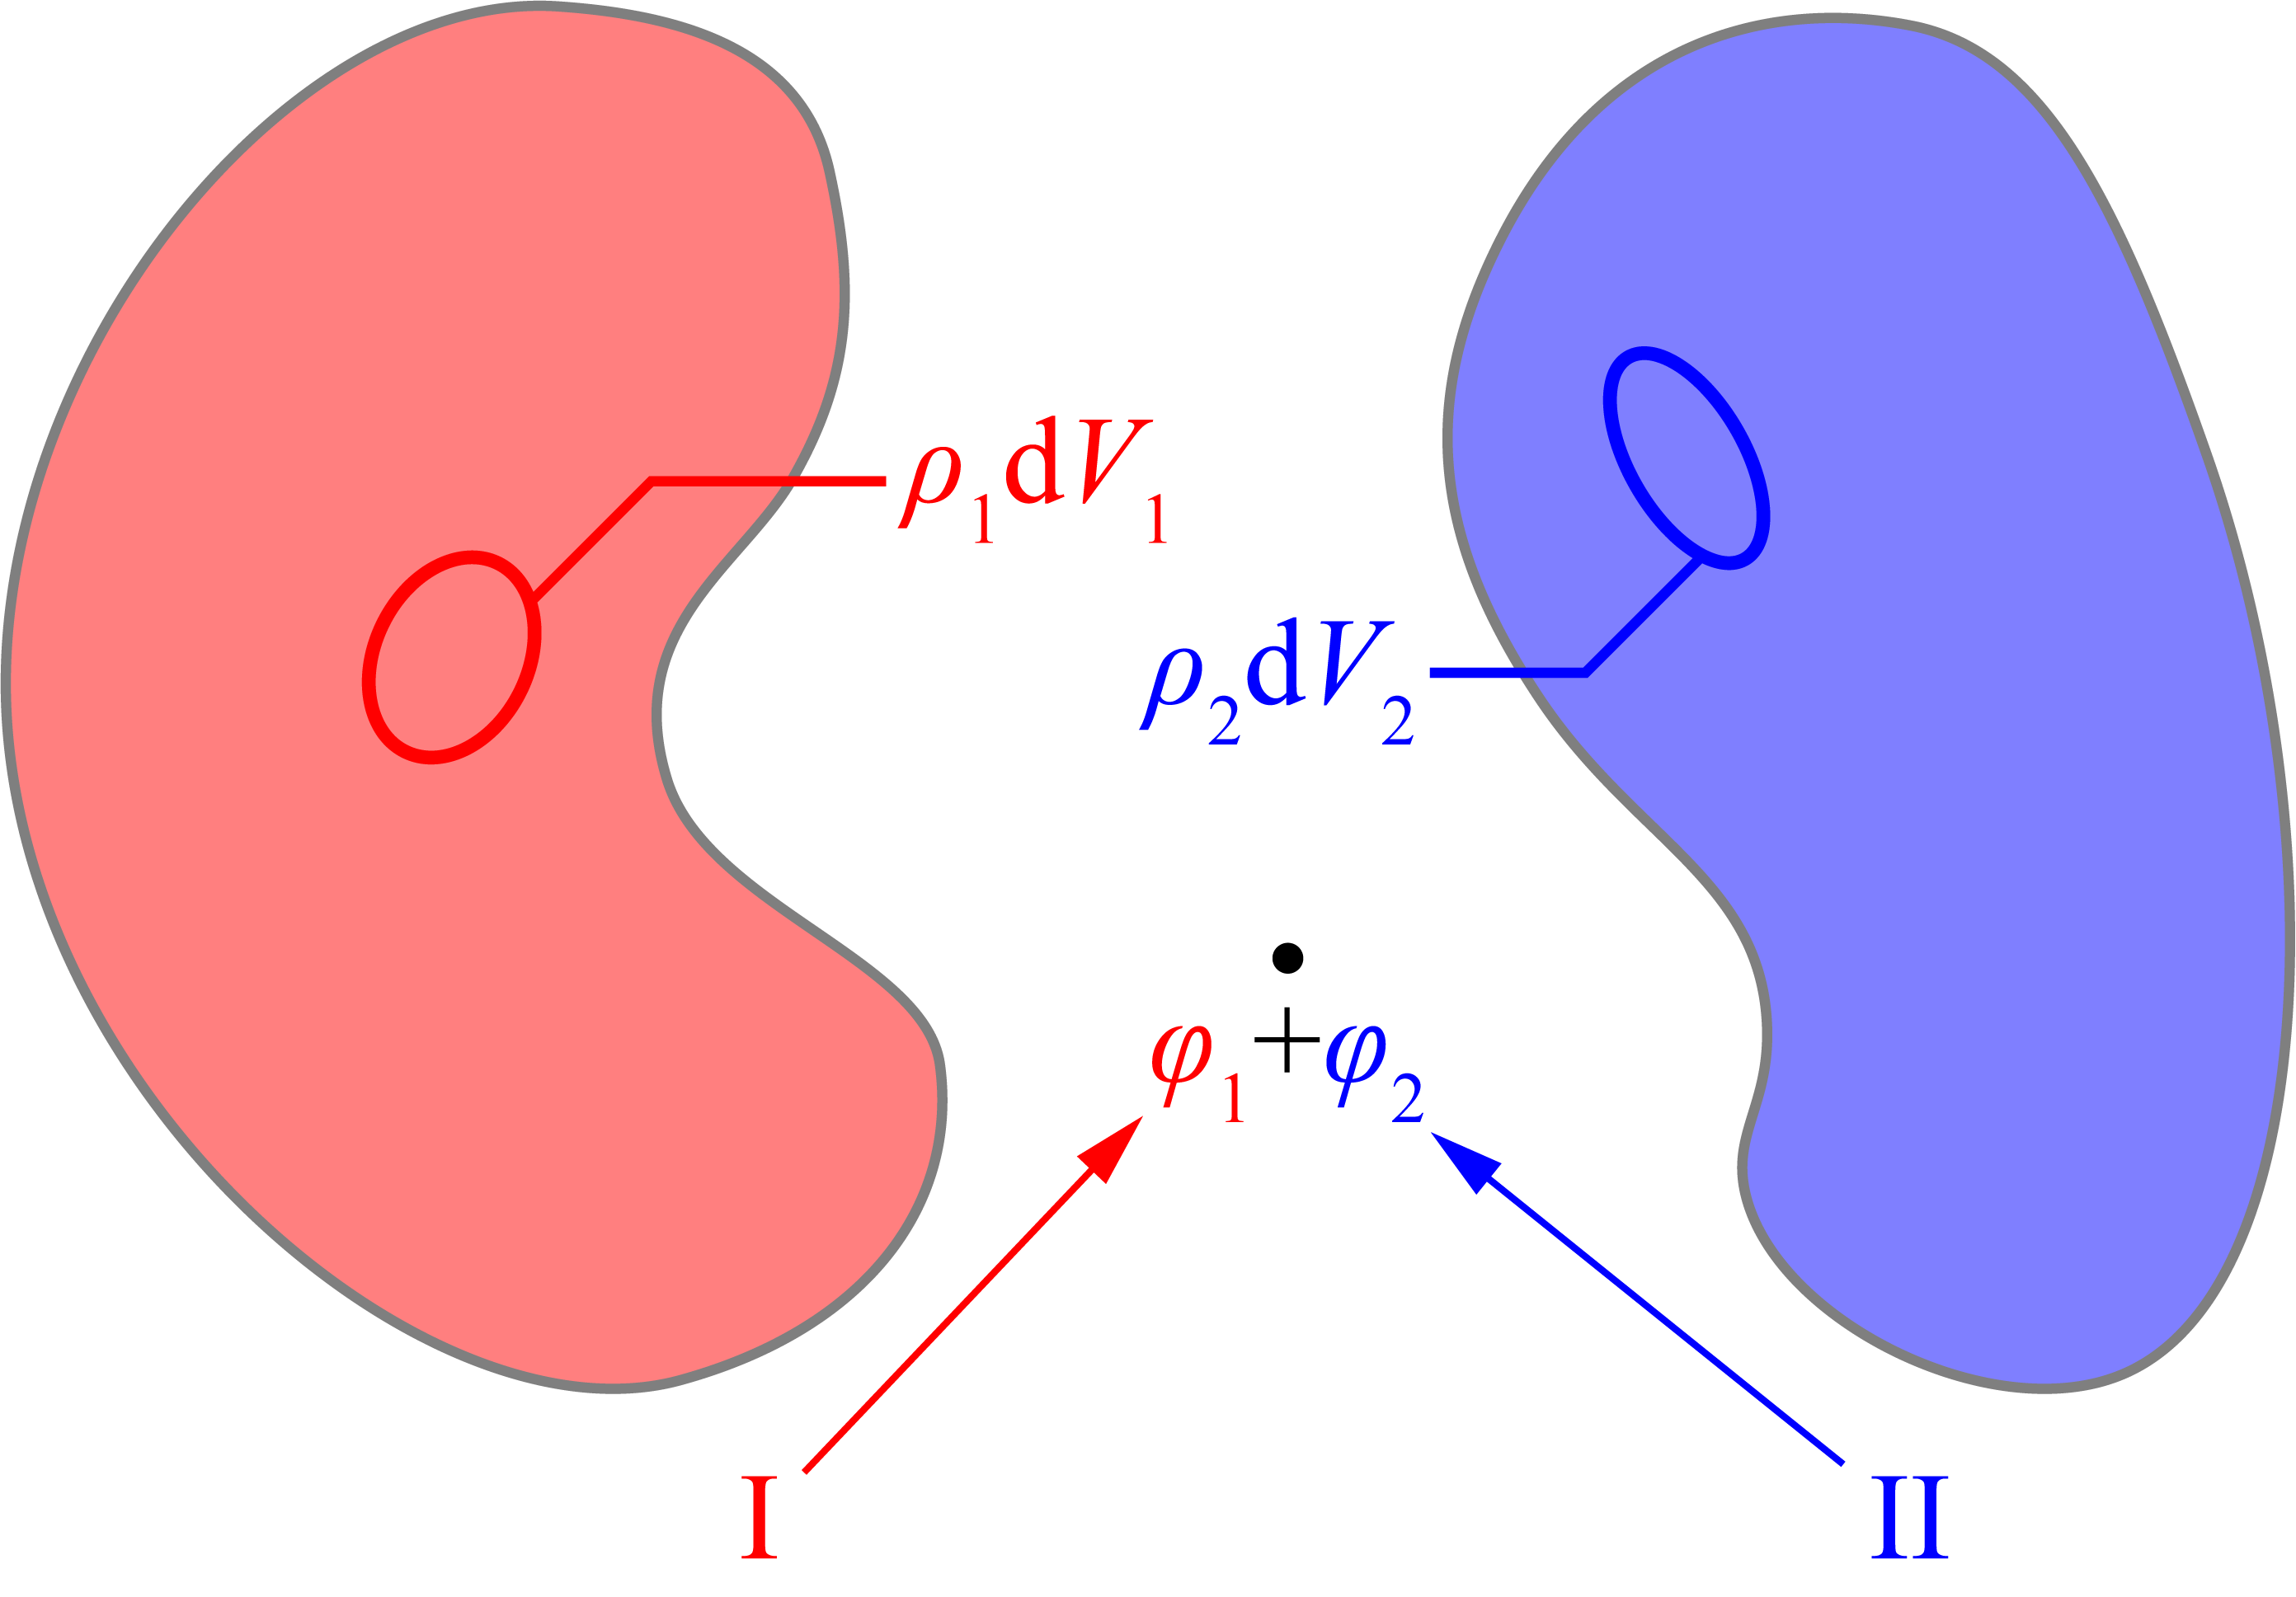
\includegraphics[width=9cm]{image/7-1-9.png}
\caption{自能与相互作用能}
\end{wrapfigure}
我们于是找到了三个能量,\,$I_1,\,I_2$是两个电荷分布体系单独存在时各自的自相互作用能,\,我们把它简称作\emph{自能}(self-energy),\,它一定是大于零的,\,这一点下一节就可以发现.\,而余下的交叉求和项就是表示两个体系之间的相互作用能.\,仔细一看不难发现一项其实就是电荷体系${\rm II}$产生的外场下电荷体系${\rm I}$的电势能,\,而另一项就是电荷体系${\rm I}$产生的外场下电荷体系${\rm II}$的电势能,\,两者仔细研究下发现其实相等:
\[I_{12}=\int\limits_{\rm I}\int\limits_{\rm II}\ke\frac{\rho_1\rho_2}{r}\ud V_1\ud V_2=\int\limits_{\rm I}\rho_1 \varphi_2\ud V_1=\int\limits_{\rm II}\rho_2 \varphi_1\ud V_2\]

这一项可以大于零也可以小于零,\,表示的是相互作用.\,现在我们试探电荷体系在外场中的电势能有了一个新的看法,\,它其实表示试探电荷体系与场源电荷体系的相互作用能,\,作为相互作用,\,它也可以反过来用场源电荷体系在试探电荷体系产生的场中的电势能来计算,\,或是对称地,\,用两者和的一半来计算.

最后让我们来看一下点电荷的自能.\,实际上在之前点电荷体系相互作用能体系中我们已经指出,\,其表达式中电荷$q_i$上电势$\phi_i$与真实电势$\varphi_i$的区别就在于没有计及点电荷在自己位置处产生的电势$\varphi_{ii}$,\,从而漏掉的项其实就是点电荷的自能:
\[I_i=\frac{1}{2}q_i\varphi_{ii}\]

这些项不会影响我们的实际计算,\,因为点电荷总被我们认为是没有内部改变的理想体系,\,我们经常把微观基本粒子做这样的抽象,\,因为它们都是小到可以忽略其尺寸.\,当粒子速度远小于光速,\,且不涉及到高能粒子反应的情况下,\,它们也的确不发生任何内部的改变,\,自能精确地保持不变.\,所以只需要计算扣除点电荷自能的相互作用能表达式,\,就能够知道有多少势能被存储在场中,\,就能够用它来写出电荷分布发生改变时释放出来的能量.

点电荷的自能如何计算呢?\,这取决于我们采取的模型.\,如果我们考虑的是一个电荷均匀分布在表面的球体,\,那么自能为:
\[I=\frac{1}{2}Q\cdot\ke\frac{Q}{r}\]

对于电子,\,如果我们认为电子的静质量全部来源于它携带的场的惯性,\,那么能够写出:
\[I=\frac{e^2}{8\pi\varepsilon_0 r}=m_e c^2\]

事实上我们并不能确定电子内部电荷分布,\,所以我们更常直接定义\emph{经典电子半径}(classical electron radius)为:
\[\frac{e^2}{4\pi\varepsilon_0 r_e}=m_e c^2\quad \Rightarrow \quad r_e=\ke \frac{e^2}{m_e c^2}=2.82\times 10^{-15} {\rm m}\]

然而这仅仅是一个方便计算的实用常数,\,并不能代表电子的真实情况!\,事实上用不带电荷的粒子与电子发生散射实验就会发现,\,电子的尺寸比这要小得多,\,上面的计算结果甚至比质子的半径还要大几倍!\,而实验更是发现电子在多种意义下就是一个点粒子,\,根本没有内部组成结构,\,十分稳定不能衰变.\,那么显然从上式发现这也面临着自能发散的问题.\,双重矛盾如何解决呢?

解决方案是量子力学的引入,\,电子不是点粒子,\,在原子尺度下电子就已经必须要由波函数描述了,\,电子没有同时确定的位置和速度,\,在原子外形成``电子云''.\,\emph{狄拉克}({\it P. Dirac})于1928年提出\emph{狄拉克方程}(Dirac equation),\,把电子像光子那样处理为一个传播的``场'',\,从而从根本上摒弃了电子作为点电荷的观点,\,电子的质量被理解为场的质量或者静能,\,而电子的电荷量被理解为与电磁场(光子)的耦合常数.\,从而把电荷作为一种物质和场物质彻底分割开来独立描述.\,还同时一并给出了电子的自旋与预言了电子的反物质:\,\emph{正电子}(positron)的存在.\,它们都被天然而巧妙的包含在一个统一的代数形式中,\,极大程度地推动了物理学理论的进展.

但这没有给出问题的全部解释,\,对于点电荷自能发散的问题这种做法仍然没有给出绝对的答案.\,经典地看一个匀速运动的经典无穷小点电荷会携带着一个发散的场共同向前运动,\,这在量子场论语言下,\,变成了电子与光子相互作用的无限可能性求和,\,从而也理所当然地引进了各种各样的发散.\,对于这些发散物理学家们发展出了各种各样的处理方法,\,但直到今天还仅仅停留在现象解释的层面,\,背后是否有更加简单的解释方法还是一个谜.


\subsection{电场能}

我们已经十分熟悉,\,电荷之间的相互作用能实际上就是场的能量.\,我们现在将给出这一说法的定域化描述.\,记得一个电荷连续分布体系的相互作用能为:
\[I=\frac{1}{2}\int\limits_V \rho\varphi\ud V\]

而又根据场与电荷之间的关系:
\[\nabla^2 \varphi=-\frac{\rho}{\varepsilon_0}\]

我们把以上积分写为:
\[I=-\frac{\varepsilon_0}{2}\int\limits_V \varphi\nabla^2\varphi\ud V\]

再根据著名的\footnote{而\emph{第二格林等式}(Green's second identity)在格林函数法解边值问题时将十分有用:
\[\nabla\cdot(\phi\nabla\psi-\psi\nabla\phi)=\phi\nabla^2\psi-\psi\nabla^2\phi\]}\emph{第一格林等式}(Green's first identity):
\[\nabla\cdot(\phi\nabla\psi)=\phi\nabla^2\psi+\nabla\phi\cdot\nabla\psi\]

我们再取$\phi,\,\psi$都为$\varphi$,\,从而:
\[\varphi\nabla^2\varphi=\nabla\cdot(\varphi\nabla\varphi)-(\nabla \varphi)^2\]

带入以上积分,\,我们得到:
\begin{align*}
I 	&=\frac{\varepsilon_0}{2}\int\limits_V (\nabla \varphi)^2\ud V-\frac{\varepsilon_0}{2}\oint\limits_{\partial V} \varphi\nabla\varphi\cdot\ud \bs{A}\\
	&=\int\limits_V \frac{\varepsilon_0}{2} \bs{E}^2 \ud V + \frac{\varepsilon_0}{2}\oint\limits_{\partial V} \varphi\bs{E}\cdot\ud \bs{A}
\end{align*}

我们总是考虑电荷分布有限的情况.\,此时最初的积分体积只要包含所有电荷即可,\,那么我们最后得到的这个恒等式就十分的有意思,\,,它将一个体系的相互作用转化为了一个量的体积分和另一个量在包含所有电荷的面上的面积分的形式.\,我们如果取体积为无穷大的全空间,\,那么考虑到随着远离电荷体系$R$处$\varphi$以至多$\dfrac{1}{R}$的方式衰减(若体系总电荷量为零则衰减更加剧烈),\,而$\bs{E}$以至多$\dfrac{1}{R^2}$的方式衰减,\,而积分面积以$R^2$的方式增加,\,故整个积分以至多$\dfrac{1}{R}$的方式衰减,\,在无穷远处这个积分的第二项就会趋于零.\,

从而我们得到了:
\[I=\int \frac{\varepsilon_0}{2} \bs{E}^2 \ud V\]

从而发现相互作用能可以用场来定域地计算.\,电场的\emph{能量密度}(energy density)为:
\[w_e=\frac{\varepsilon_0}{2} \bs{E}^2\]

场的能量不再由电荷造成,\,而是由场自己的场强去定义,\,以后还会进一步证明,\,场在一点处对电荷有力的作用,\,将会使场的动量密度发生改变,\,而对电荷有做功,\,将会影响这一点处的能量密度.


\section{电荷体系}

讨论若干电荷体系对于之后问题的理解是大有帮助的.\,这些包括:

\subsection{电偶极子}

\begin{wrapfigure}[11]{o}[0pt]{7cm}
\centering
\vspace{-2cm}
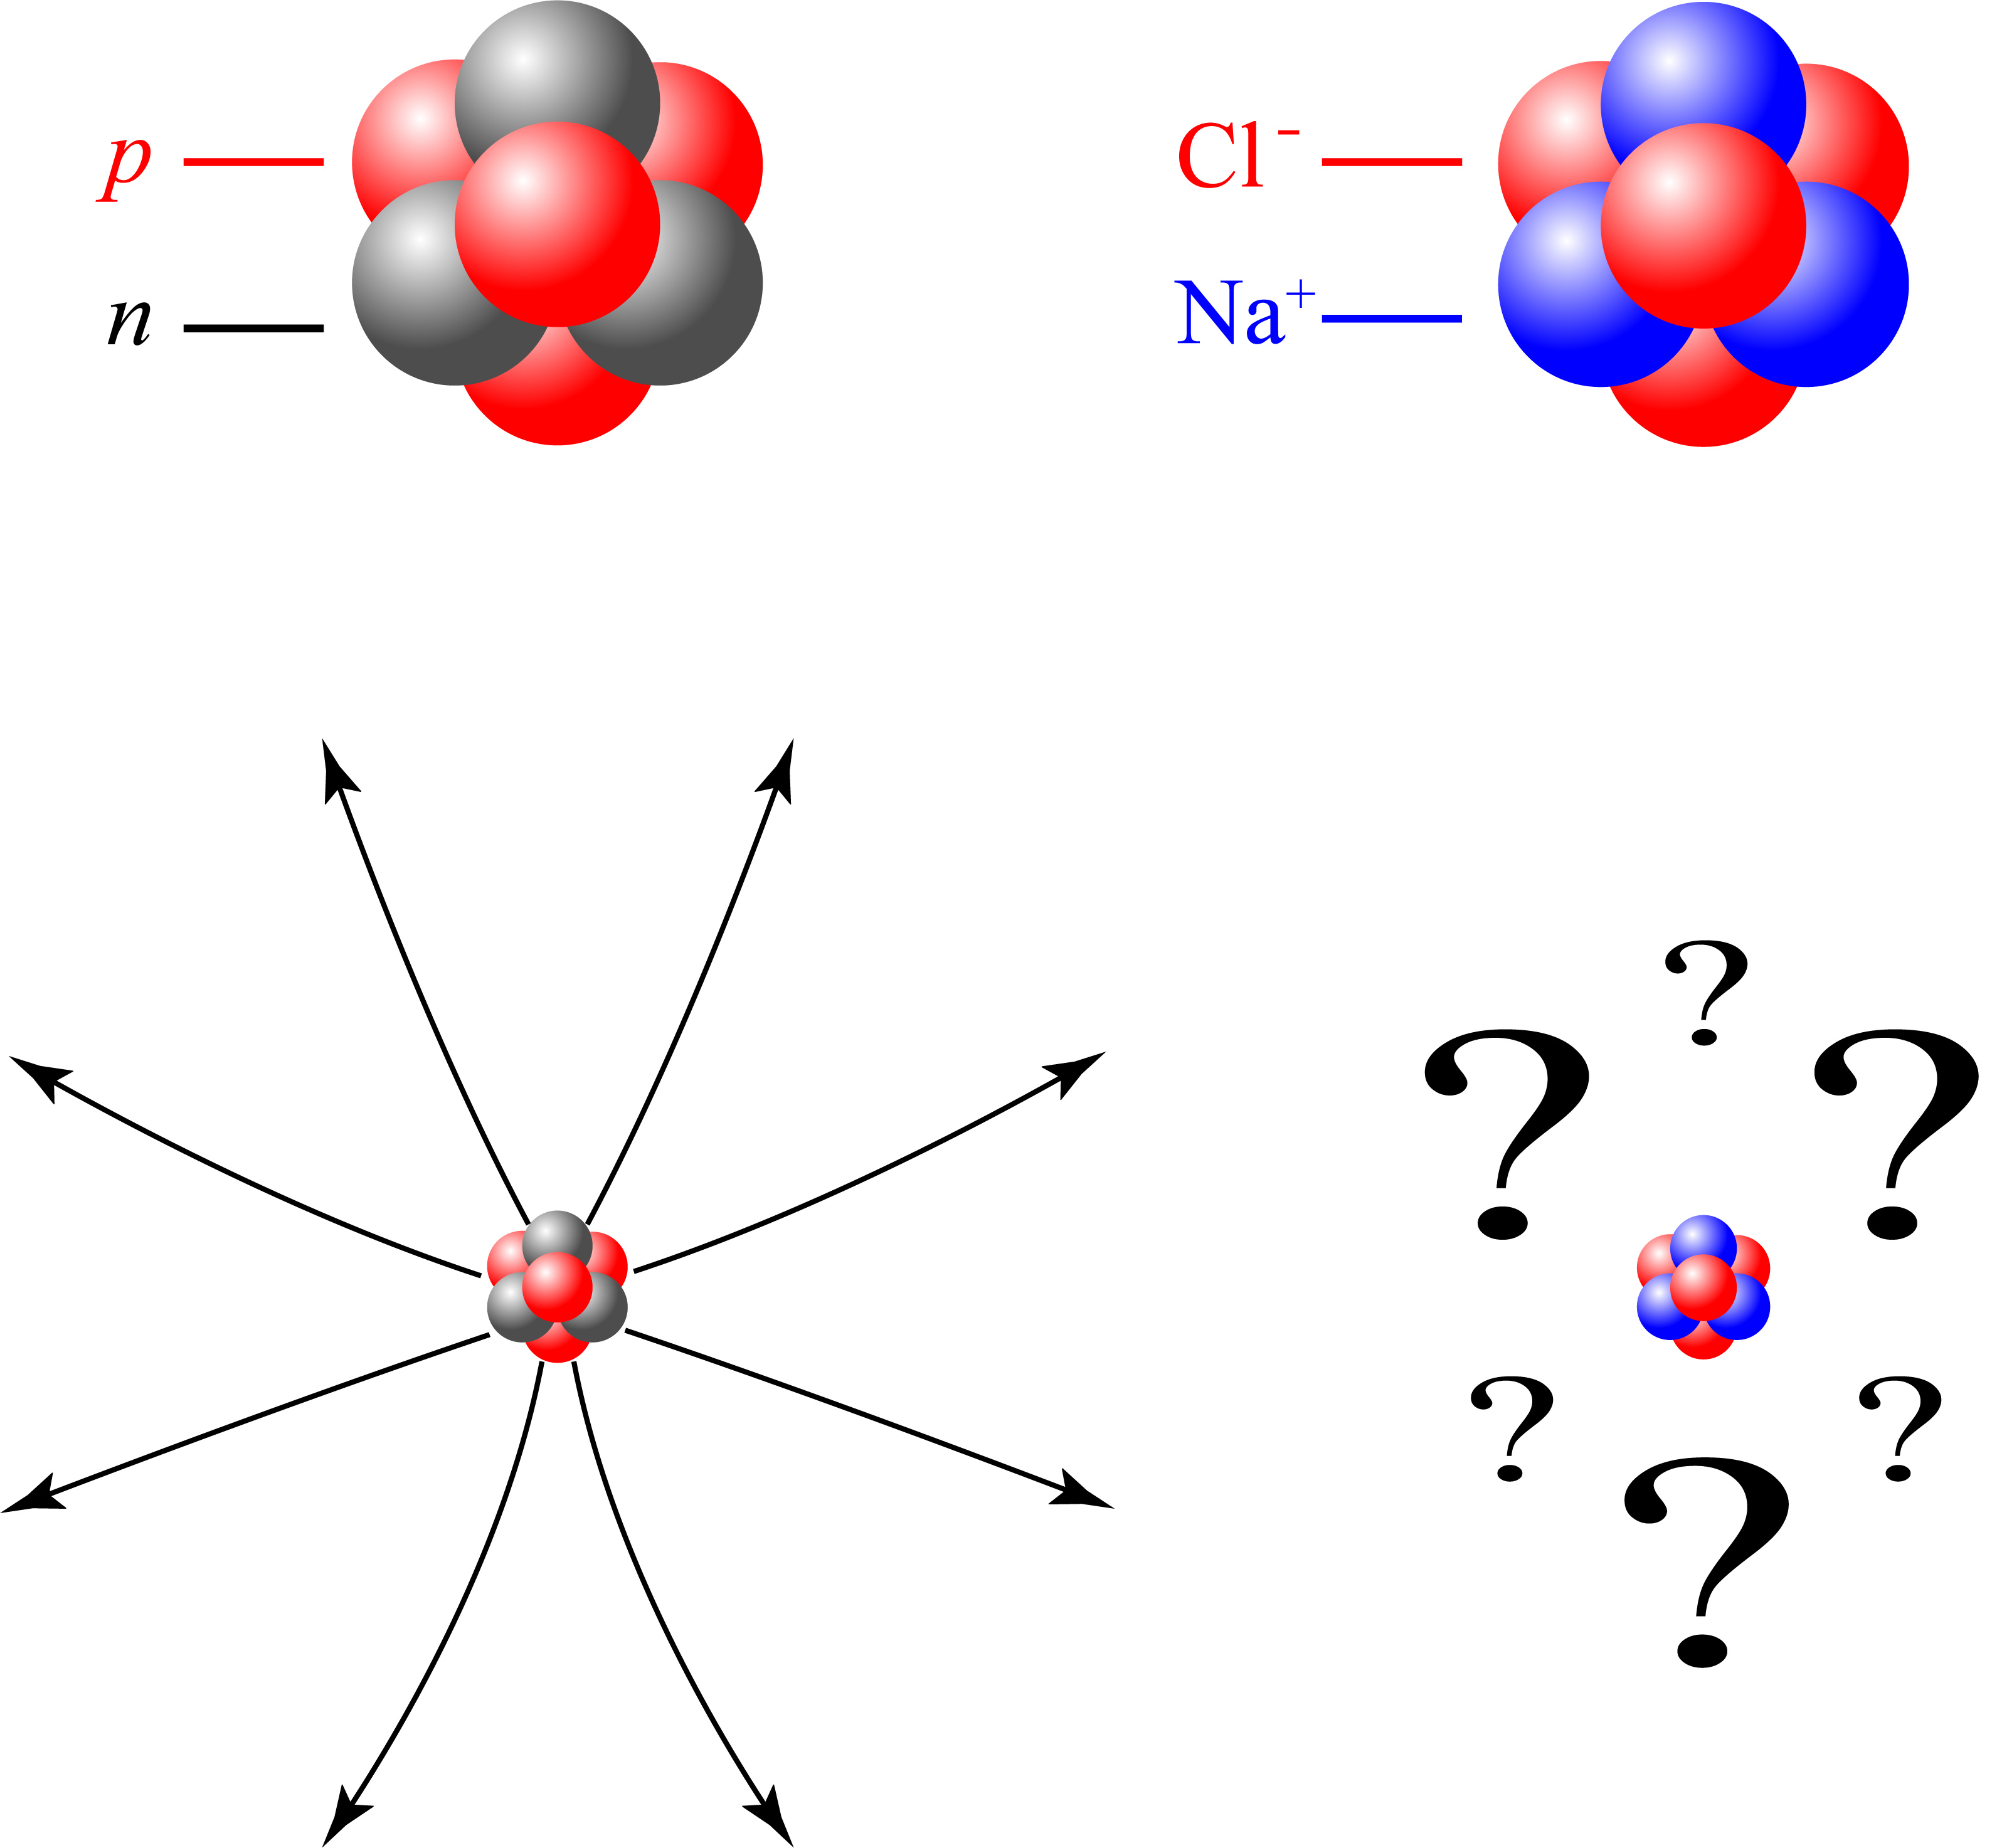
\includegraphics[width=7cm]{image/7-1-10.png}
\caption{远方的场}
\end{wrapfigure}
我们都知道一个电荷体系如果带电,\,那么尽管在离电荷体系很近处电场分布不均匀,\,但离开分布电荷足够远处的场强却总是趋于一个点电荷的电场.\,常见的情况发生在原子核中,\,原子核由质子和中子组成,\,质子带电而中子不带电.\,原子核内电荷分布总是不均匀的,\,但在考虑外界电子受力时总是将其产生的场视为库仑场.\,这是因为电子典型半径:\,玻尔半径与原子核的尺寸比差了$5$个数量级.\,在这个距离处电场完全可以看成是库仑场,\,它与库仑场的偏离将作为一个可以忽略的小量而不去考虑.

但类似的,\,我们将考虑到很多不带净电荷的电荷分布体系,\,它们在近处产生一个不均匀的电场,\,而在远处产生的电场却总是存在着某些规律.\,这个问题有重要的实用价值.\,比如我们如果从${\rm NaCl}$晶体中取出一小块来,\,它的总电量总是为零,\,但由于晶体的变形等因素导致正负电荷产生的电场并不能完全抵消,\,这个电场将会与晶体的动力学耦合,\,极大地影响晶体的动力学特征.\,又比如很多分子实际上属于\emph{极性分子}(polar molecule),\,由于原子的\emph{电负性}(electronegativity)差异,\,原子间的键合具有极性,\,在很多情形下一个原子对公用电子对的吸引能力更强,\,导致电子集中在一个原子一侧.\,从而负电荷的中心向这个原子位移.\,只要分子结构上的对称性不会使得键的极性不会相互抵消,\,整个分子就会显示出极性来,\,它是溶液中溶剂溶解机理的关键,\,也会影响物质的熔点,\,沸点,\,极化率等等关键的物理特性.

\begin{wrapfigure}[11]{o}[0pt]{6cm}
\centering
\vspace{-0.6cm}
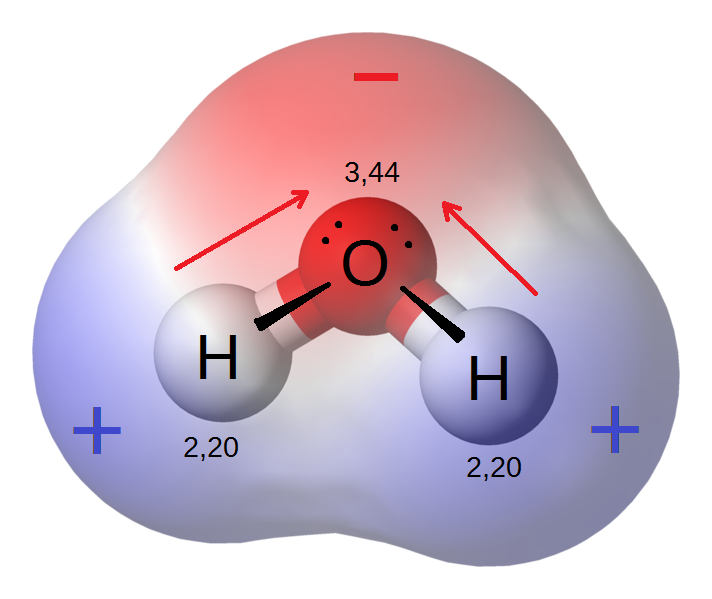
\includegraphics[width=6cm]{image/7-1-11.png}
\caption{水分子极性}
\end{wrapfigure}
所以我们关心总电荷量为零的体系在很远处产生的电场,\,理论上我们可以采取更完整的\emph{多极展开}(multipole expansion)的做法,\,在很多情况下\emph{电偶极项}(dipole term)成为了这种情形下的\emph{领头项}(leading order).\,我们定义小范围分布电荷体系中所有正电荷的``中心''和负电荷的``中心'':
\[\bs{r}_+=\frac{\displaystyle\sum_{q_i>0} q_i \bs{r}_i}{Q}\quad,\quad Q=\sum_{q_i>0} q_i\]
\[\bs{r}_-=\frac{\displaystyle\sum_{q_i<0} q_i \bs{r}_i}{-Q}\quad,\quad -Q=\sum_{q_i<0} q_i\]

而体系的\emph{电偶极矩}(dipole moment)就被定义为由负电荷指向正电荷的矢量:
\[\bs{d}=Q(\bs{r}_+-\bs{r}_-)\]

或者写为:
\[\bs{d}=\sum_{i} q_i \bs{r}_i\]

求和遍及所有电荷,\,无论正负.\,由于总电荷量是零,\,不难验证这个矢量与坐标原点的选取无关,\,为了纪念物理学家\emph{德拜}({\it P. Debye})在分子物理领域的相关开创性工作,\,它一般使用以德拜命名的单位,\,它是一个高斯制单位:
\begin{align*}
1 \;{\rm D} 	&=10^{-18} \;{\rm statC\cdot cm} \\
			&=\frac{1}{299792458}\times 10^{-21} \;{\rm C\cdot m} \\
			&=3.34\pow{-30} \;{\rm C\cdot m} \\
			&=0.208 \;{\rm e\cdot \angstrom}
\end{align*}


\begin{wrapfigure}[8]{o}[0pt]{4cm}
\centering
\vspace{-2.5cm}
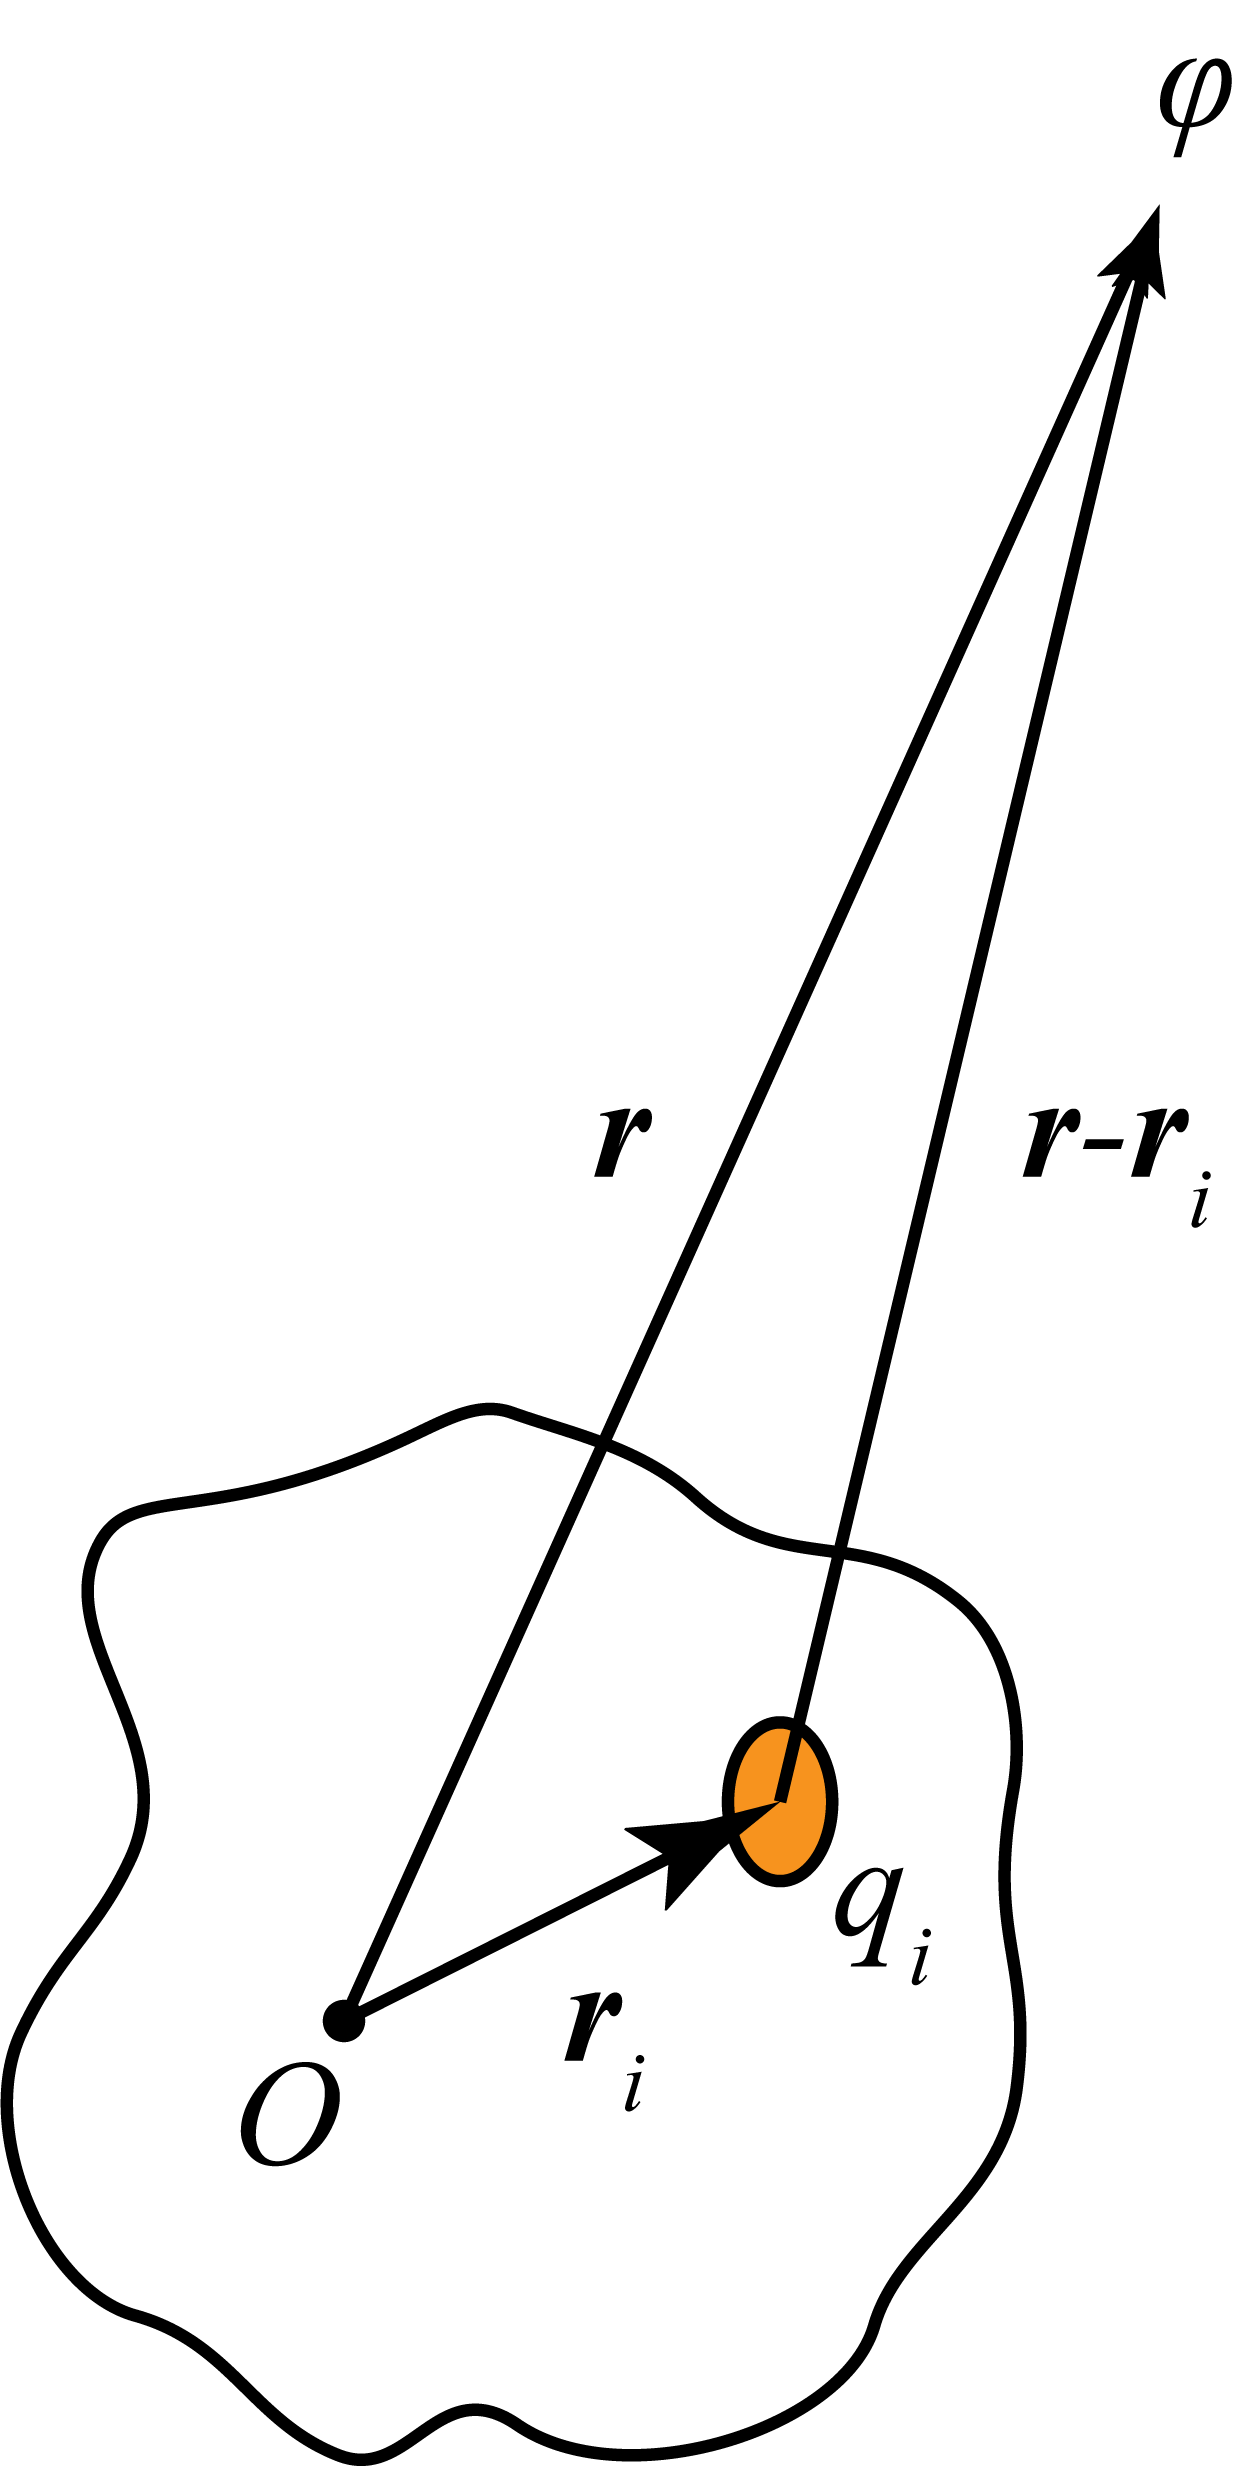
\includegraphics[width=4cm]{image/7-1-12.png}
\caption{偶极展开}
\end{wrapfigure}
为何定义这样的一个矢量呢?\,我们考察在原点附近分布了一个电荷体系$\{q_i ,\, \bs{r}_i\}$,\,那么在很远处产生的电势应该为:
\[\varphi(\bs{r})=\sum_i \ke \frac{q_i}{|\bs{r}-\bs{r}_i|}\]

而对于分母中的矢量的模,\,我们考虑到$|\bs{r}|\gg|\bs{r}_i|$,\,可以做如下近似:
\begin{align*}
\frac{1}{|\bs{r}-\bs{r}_i|} 	&=[(\bs{r}-\bs{r}_i)^2]^{-\frac{1}{2}}=(\bs{r}^2-2\bs{r}_i\cdot\bs{r}+\bs{r}_i^2)^{-\frac{1}{2}} \\
								&\approx (r^2-2\bs{r}_i\cdot\bs{r})^{-\frac{1}{2}}=\frac{1}{r}(1-2\frac{\bs{r}_i\cdot\bs{r}}{r^2})^{-\frac{1}{2}} \\
								&\approx \frac{1}{r}(1+\frac{\bs{r}_i\cdot\bs{r}}{r^2})=\frac{1}{r}+\frac{\bs{r}}{r^3}\cdot \bs{r}_i \\
								&=\frac{1}{r}+\frac{\bs{e}_r}{r^2}\cdot \bs{r}_i
\end{align*}

代入求和表达式,\,得:
\[\varphi(\bs{r})\approx \ke \frac{\displaystyle\sum_i q_i}{r}+\ke \frac{\bs{e}_r\cdot\displaystyle\sum_i q_i \bs{r}_i}{r^2}\]

第一项求和由于总电荷量为零放弃了成为领头项的机会,\,而第二项凸显了出来,\,根据我们之前定义的电偶极矩,\,它实际上就是:
\[\varphi(\bs{r})=\ke \frac{\bs{e}_r\cdot\bs{d}}{r^2} \quad (r\gg d)\]

我们取了等号,\,条件是我们考察的点的矢径$r$远大于电荷分布的平均尺寸$d$.\,而理论上常常构造一种十分独特的体系,\,我们让一对电量为$+Q$与$-Q$严格相等的点电荷相离$\bs{r}_+-\bs{r}_-=\bs{l}$,\,再令$Q\to\infty$而$\bs{l}\to \bs{0}$,\,而保持$\bs{p}=Q\bs{l}$的值保持不变,\,其极限就是抽象的模型:\,\emph{点电偶极子}(point dipole),\,它在除原点外,\,全空间产生的电势都可以用上式来表示.\,这也是我们以后讨论的中心.\,如果在点电偶所在空间点建立球极坐标系,\,而把电偶极矩矢量指向的方向作为极轴,\,我们可以写出电势为:
\[\varphi(r,\,\theta)=\ke\frac{p\cos\theta}{r^2}\]
\begin{wrapfigure}[11]{o}[0pt]{7cm}
\centering
\vspace{-0.5cm}
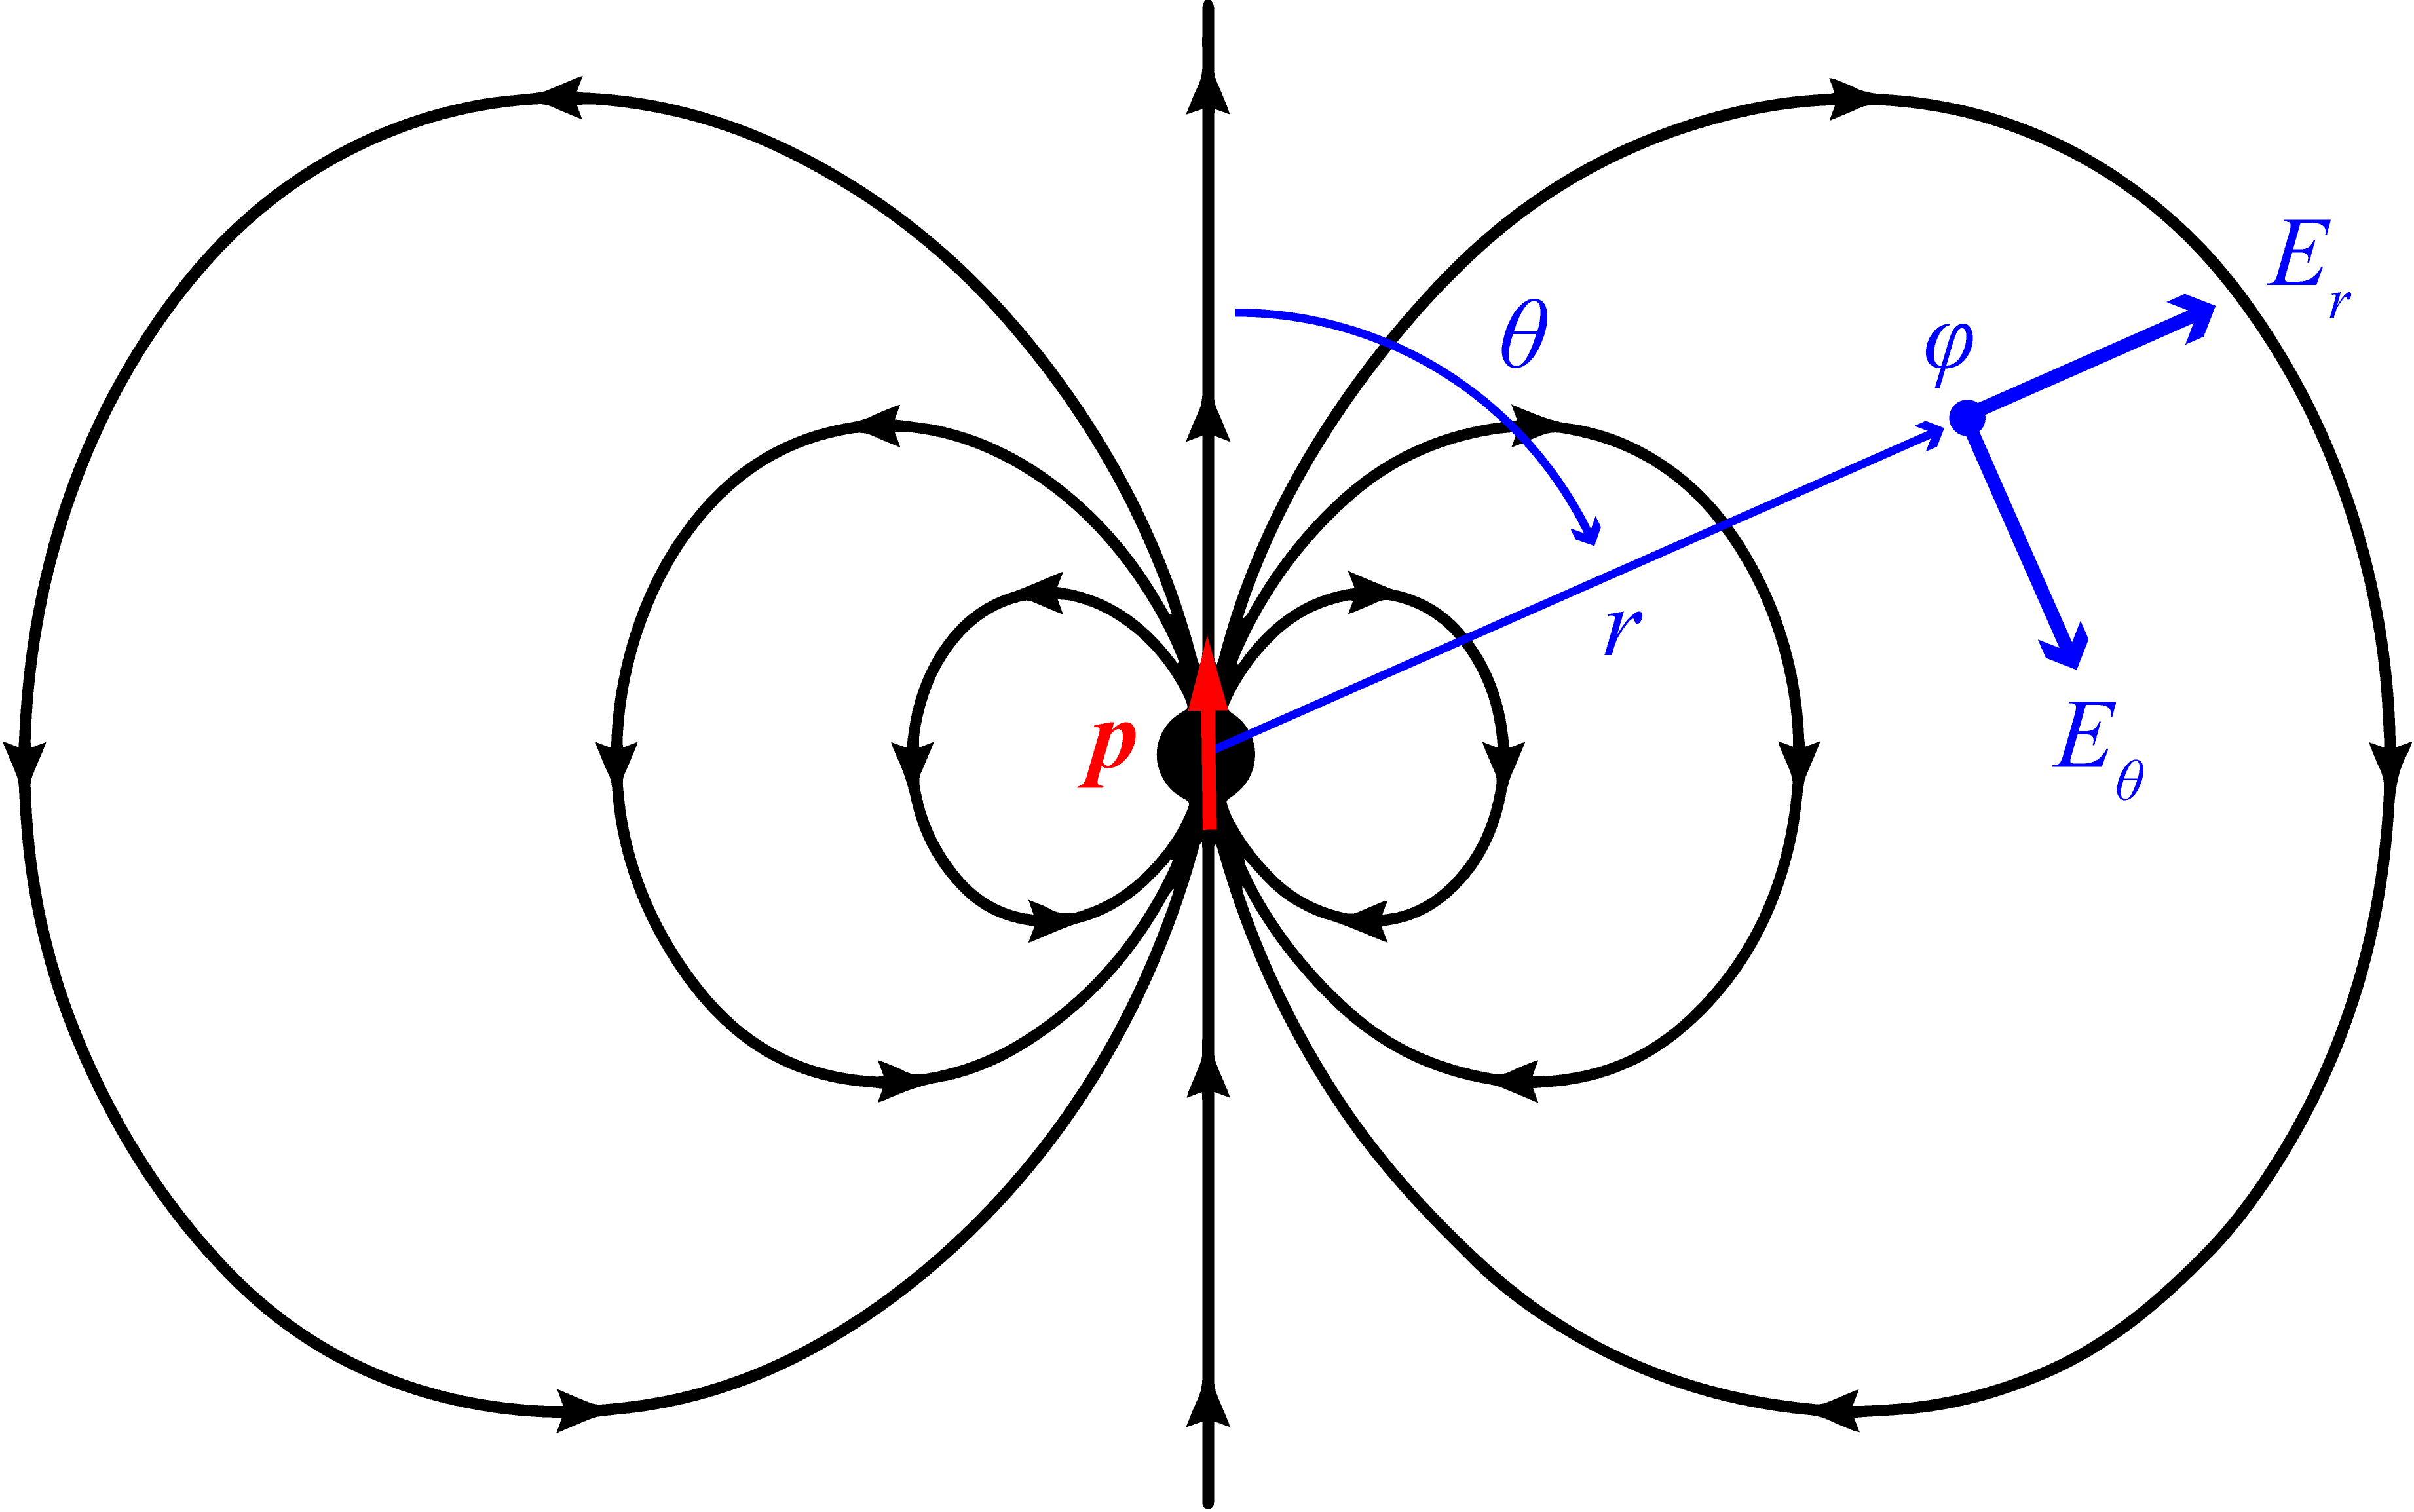
\includegraphics[width=7cm]{image/7-1-13.png}
\caption{点电偶极子的场}
\end{wrapfigure}
这是一个与半径平方反比的电势,\,它与角度有关.\,利用球坐标下梯度算符的表示:
\[\nabla=\bs{e}_r \frac{\partial}{\partial r} +\frac{1}{r}\frac{\partial}{\partial \theta}+\frac{1}{r\sin\theta}\frac{\partial}{\partial \phi}\]

我们计算出点电偶极子的电场来:
\[E_r(r,\,\theta)=\ke\frac{2p\cos\theta}{r^3}\]
\[E_\theta(r,\,\theta)=\ke\frac{p\sin\theta}{r^3}\]

可见电场倒是三次反比了.\,它比点电荷产生的场随距离减少地更快.\,理论研究经常会把以上两个分量式组合为一个矢量式,\,不难验证\footnote{这个表达式对原点以外的点适用,\,如果考虑原点的奇异电场特性,\,并引入\emph{狄拉克德尔塔函数}(Dirac delta function),\,则更准确的表达式为:
\[\bs{E}=\ke \frac{3(\bs{e}_r\cdot\bs{p})\bs{e}_r-\bs{p}}{r^3}-\frac{\bs{p}}{3\varepsilon_0}\delta^3(\bs{0})\]}
\[\bs{E}=\ke \frac{3(\bs{e}_r\cdot\bs{p})\bs{e}_r-\bs{p}}{r^3}\]

如果考虑电偶极子在外场中的情形,\,采用两电荷分布极限为点电偶极子的结果,\,我们很容易发现它的电势能为:
\[V=Q(\varphi_+-\varphi_-)=Q\bs{l}\cdot\nabla\varphi=-\bs{p}\cdot\bs{E}\]

注意到根据电势能的含义,\,这个能量是不包含构成电偶极子的两电荷之间的相互作用能的,\,而在电偶极子在电场中发生位移的过程中我们也应该不能让电偶极子发生结构的改变:\,即,\,$\bs{p}$的大小不能改变,\,但$\bs{p}$的方向,\,位置都可以发生改变,\,随着这两个剩余自由度发生变化,\,电场对电偶极子做的虚功$-\delta V=\delta[\bs{p}\cdot\bs{E}(\bs{r})]$就被理解为力矩与受力:
\[\delta \bs{r}=\bs{0},\;\delta \bs{p}=\delta \bs{\theta}\times \bs{p}:\; -\delta V=\bs{M}\cdot \delta\bs{\theta}\quad \Rightarrow \quad \bs{M}=\bs{p}\times\bs{E}\]
\[\delta \bs{r}\neq\bs{0},\;\delta \bs{p}=0:\; -\delta V=\bs{F}\cdot \delta\bs{r}\quad \Rightarrow \quad \bs{F}=\bs{p}\cdot\nabla\bs{E}\]

其中表达式$\bs{p}\cdot\nabla\bs{E}$的含义为取沿$\bs{p}$方向的矢量场$\bs{E}$的方向导数.\,以后会提到导体或电介质颗粒将会在外电场下感应或极化出一个电偶极子来:
\[\bs{p}=\alpha \bs{E}\]

把此式代入受力公式,\,我们发现:
\[\bs{M}=0\quad;\quad \bs{F}=\frac{\alpha}{2}\nabla{E^2}\]

这也就是我们常说的电场有能够吸引轻小物体的本领的解释,\,我们发现这些小物体在外电场中的受力方向总是指向电场强度大小增加的方向的,\,而与电场强度方向关系不大.

\subsection{电荷密度}

\begin{figure}[H]
\centering
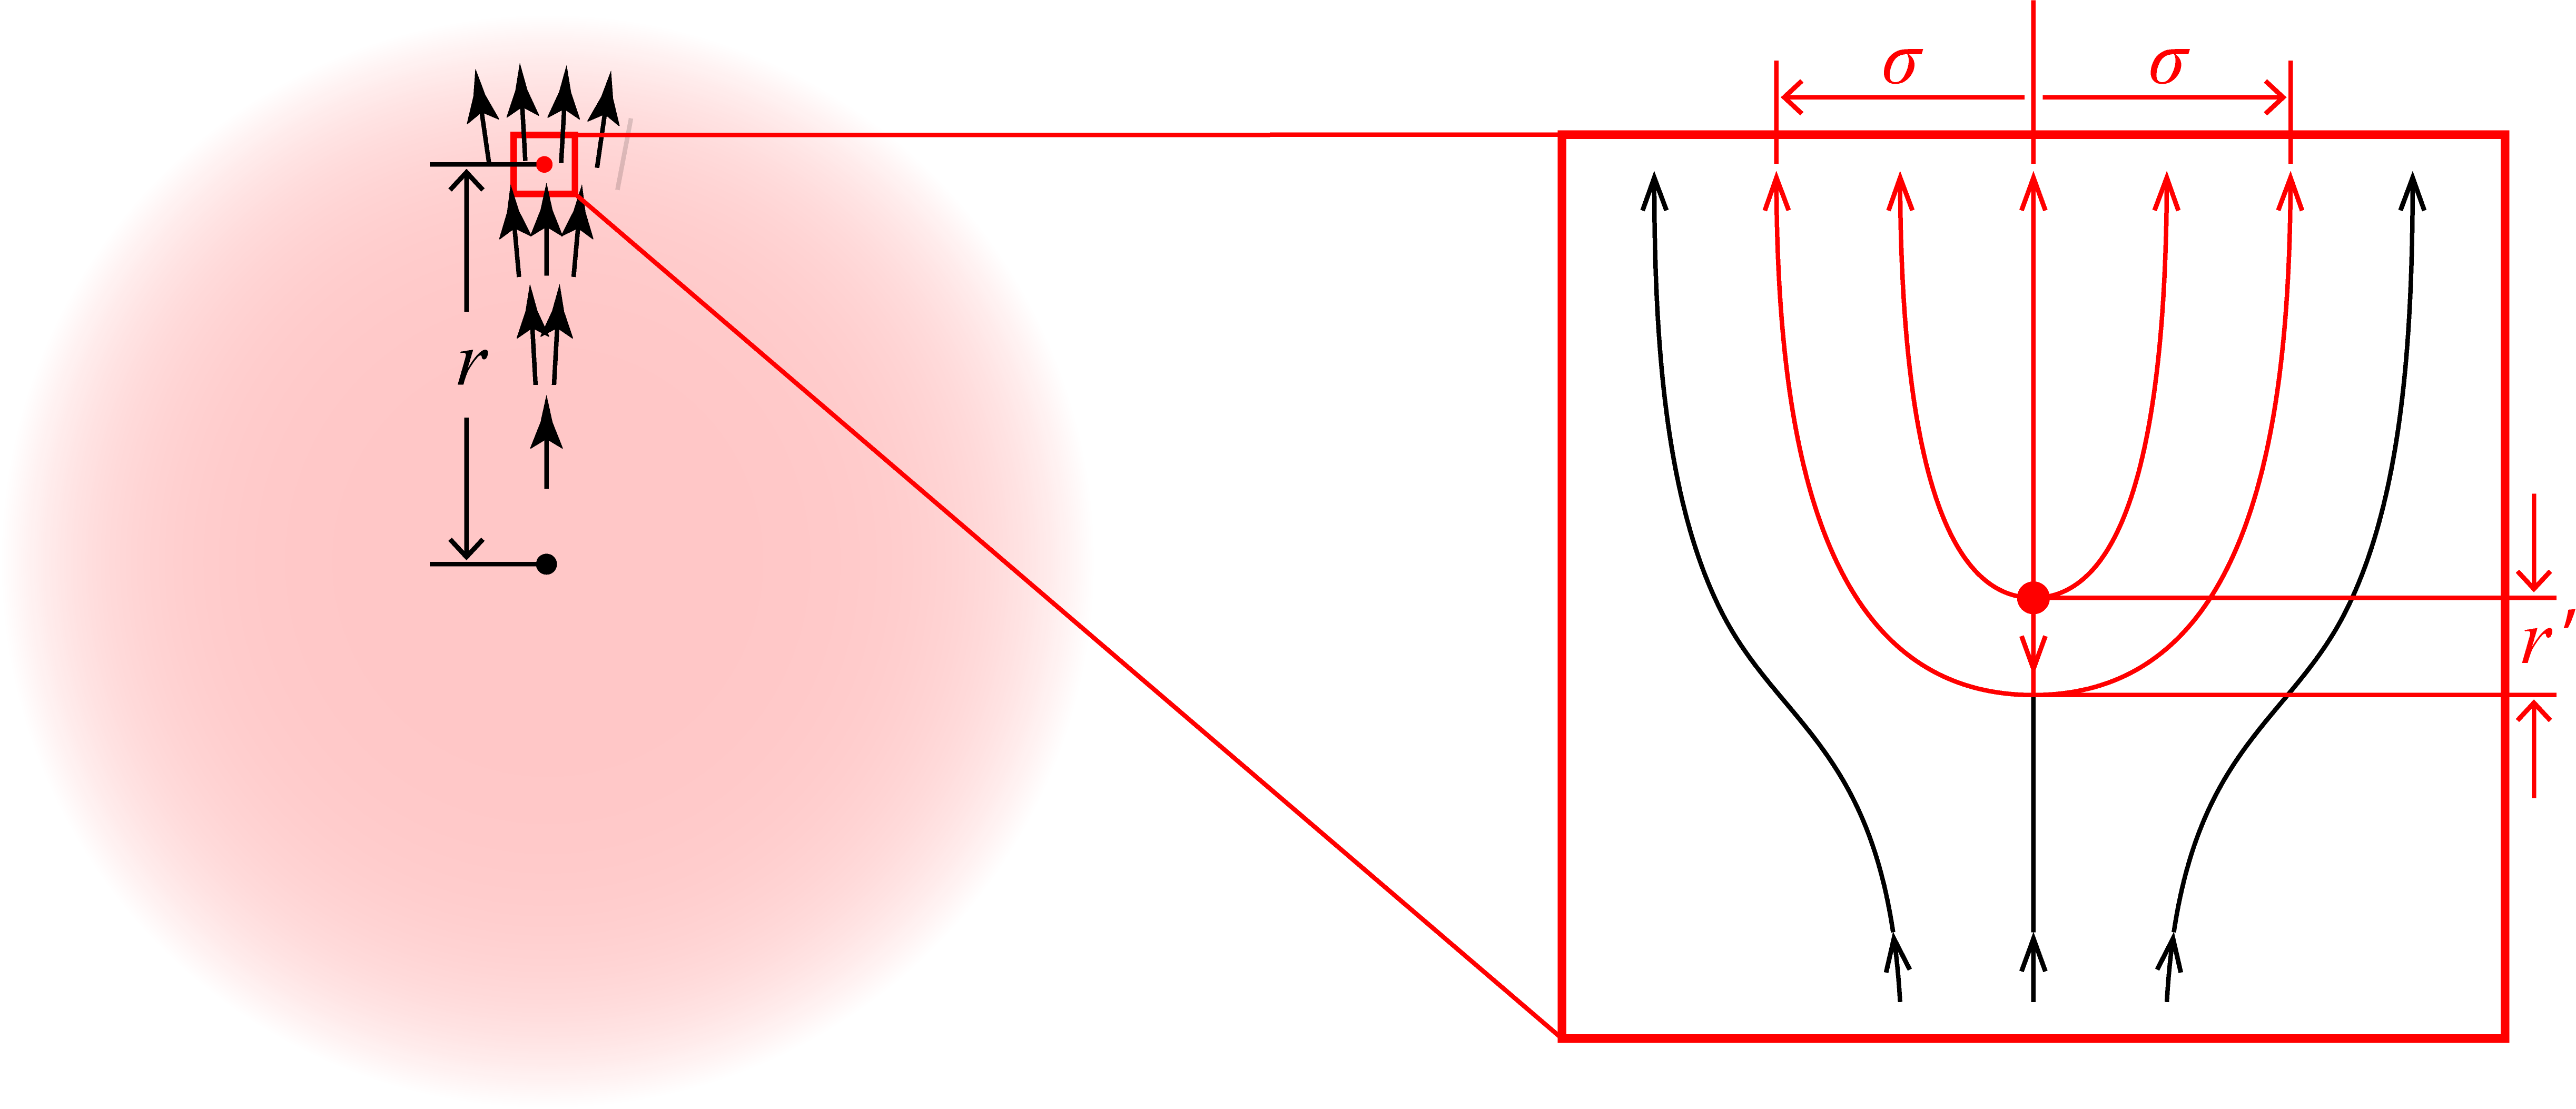
\includegraphics[width=0.5\textwidth]{image/7-1-14.png}
\caption{连续分布点电荷产生平均电场}
\end{figure}
我们经常会用到连续分布的电荷这样的说法,\,把电荷分布写成一个$\rho(\bs{r})$的形式,\,表示每一个体积元$\ud V$中含有的电荷量为$\rho\ud V$.\,这种做法在分析理论问题时发挥了很重要的作用,\,但是它却并不实际.\,实际电荷分布在很小的尺度看来永远是不连续的,\,经典情况下一般可以视为由基本电荷量的点粒子产生的.\,那么正如前述,\,在这样的情况下电荷密度被理解为:
\[\rho=\sum_i n_iq_i\]

更难理解的此时电场强度的定义.\,让我们考虑一个均匀带点的球,\,此时球外的电场强度自然可以简单的按$\dfrac{Q}{4\pi\varepsilon_0 r^2}$来计算.\,若内部的电场若按照完全的连续电荷分布来计算,\,给出了:
\[\bs{E}=\frac{\rho \bs{r}}{3\varepsilon_0}\]

的结果.\,但这个结果忽略了电荷的离散性,\,我们如果认为这个球是由电荷数密度为$n$,\,电荷量为$q$的大量点电荷构成.\,那么设在半径为$r$处的电场与单个点电荷在距中心为$r'$处的电场相等.\,我们可以得到:
\[\frac{nqr}{3\varepsilon_0}=\frac{q}{4\pi\varepsilon_0 r'^2}\]

如果一个电荷的平均占据体积视为球体,\,半径为$R$,\,那么电荷数密度与它的关系为:
\[n\cdot\frac{4}{3}\pi R^3=1\]

这样就得到:
\[\frac{r'}{R}=\sqrt{\frac{R}{r}}\]

或者用$r$区域内包含的电荷数量$N=\left.\dfrac{4}{3}\pi r^3\right/\dfrac{4}{3}\pi R^3$,\,得到:
\[r'=\frac{R}{N^{1/6}}\]

还有一种看法是考察一个电荷发出的电场线在远方形成匀强电场以后的截面:
\[\frac{nqr}{3\varepsilon_0}\cdot \pi\sigma^2=\frac{q}{\varepsilon_0}\]

我们很容易发现:
\[\sigma=2r\]

也就是说,\,离开中心区域越远,\,包含的总电荷数量越多,\,该处点电荷产生的电场相对与由内部大量电荷积累而来的大的几乎均匀的电场相比就足够地小.\,点电荷使得外电场偏离均匀的空间范围就远小于电荷与电荷之间的间距,\,使得电荷之间的空间就可以视为一个几乎均匀的场.

最后我们总结,\,在用堆放点电荷的方式来得到一个电荷密度时,\,尽管微观来看产生的电磁场仍然很不均匀,\,但我们可以抽象出来每一点的平均场强的概念.\,它的意义有二:\,一是下一节即将证明的该点局部微元体积内电场的平均值.\,二是如果保证电荷密度不变电荷无限分散的极限情形下该点处的实际场强.\,它的算法依然是:
\[\bs{E}=\int\limits_{V'} \ke \frac{\rho \bs{e}_{\bs{R}}}{\bs{R}^2} \ud V'\]

而既然电场算法与真实的连续分布的电荷没有区别.\,电势,\,局部电荷受力体密度就仍然可以这样计算:
\[\varphi=\int \ke\frac{\rho}{|\bs{R}|}\ud V'\quad ,\quad \bs{f}=\rho \bs{E}\]

\subsection{极化强度}

往往,\,平常状态下的物质的真实情况是,\,所有局部都不是由单一的点电荷单元堆积而成.\,就比如液体的水,\,它的重复单元是电中性的水分子.\,尽管电中性,\,对外表现出偶极子,\,在原场情况下近似为点电偶极子,\,便是其电势电场的领头项.\,故我们需要考虑的实际情况是:\,单位体积内有$n(\bs{r})$个偶极矩为$\bs{p}(\bs{r})$的点电偶极子.\,这里$\bs{p}$不会是常矢量,\,首先其方向往往随着空间位置逐渐在改变,\,而每个电偶极子的电偶极矩大小亦可能因为极化程度的不同而有所区别,\,下一章我们要介绍的位移极化就是这样的情形.\,我们将数密度$n$与电偶极矩$\bs{p}$相乘,\,得到单位体积内的电偶极矩,\,即\emph{极化强度}(polarization density):
\[\bs{P}=n\bs{p}\]

对于连续情况,\,我们发现电势应该用电偶极子的电势进行体积分来得到:
\[\varphi=\int \ke \frac{\bs{P}\cdot \bs{e}_{\bs{R}}}{\bs{R}^2}\ud V' \quad ,\quad \bs{R}=\bs{r}-\bs{r}'\]

然而我们发现以下等式是成立的:
\[\nabla'=\bs{e}_x\frac{\partial}{\partial x'}+\bs{e}_y\frac{\partial}{\partial y'}+\bs{e}_z\frac{\partial}{\partial z'}\]
\[\nabla'\cdot\frac{\bs{P}}{|\bs{R}|}=\frac{\nabla'\cdot \bs{P}}{|\bs{R}|}+\bs{P}\cdot\nabla'\frac{1}{|\bs{R}|}\]
\[\nabla\frac{1}{|\bs{R}|}=\nabla\frac{1}{|\bs{r}-\bs{r}'|}=-\frac{\bs{r}-\bs{r}'}{|\bs{r}-\bs{r}'|^3}=-\frac{\bs{e}_{\bs{R}}}{\bs{R}^2}\quad,\quad \nabla'\frac{1}{|\bs{R}|}=\nabla'\frac{1}{|\bs{r}-\bs{r}'|}=-\frac{\bs{r}'-\bs{r}}{|\bs{r}'-\bs{r}|^3}=\frac{\bs{e}_{\bs{R}}}{\bs{R}^2}\]
\[\Rightarrow\quad \frac{\bs{P}\cdot \bs{e}_{\bs{R}}}{\bs{R}^2}=\nabla'\cdot\frac{\bs{P}}{|\bs{R}|}-\frac{\nabla'\cdot \bs{P}}{|\bs{R}|}\]

这样我们就得到在区域$V'$内存在极化矢量$\bs{P}$时在全空间产生的电势的公式:
\begin{align*}
\varphi 	&=\int\limits_{V'}\ke (\nabla'\cdot\frac{\bs{P}}{|\bs{R}|}-\frac{\nabla'\cdot \bs{P}}{|\bs{R}|})\ud V'\\
			&=\oint\limits_{\partial V'} \ke \frac{\bs{P}\cdot\ud \bs{A}'}{|\bs{R}|}+\int\limits_{V'}\ke\frac{-\nabla'\cdot \bs{P} \ud V'}{|\bs{R}|}\\
			&=\oint\limits_{\partial V'} \ke \frac{\sigma_P\ud A'}{|\bs{R}|}+\int\limits_{V'}\ke\frac{\rho_P \ud V'}{|\bs{R}|}
\end{align*}

\begin{figure}[H]
\centering
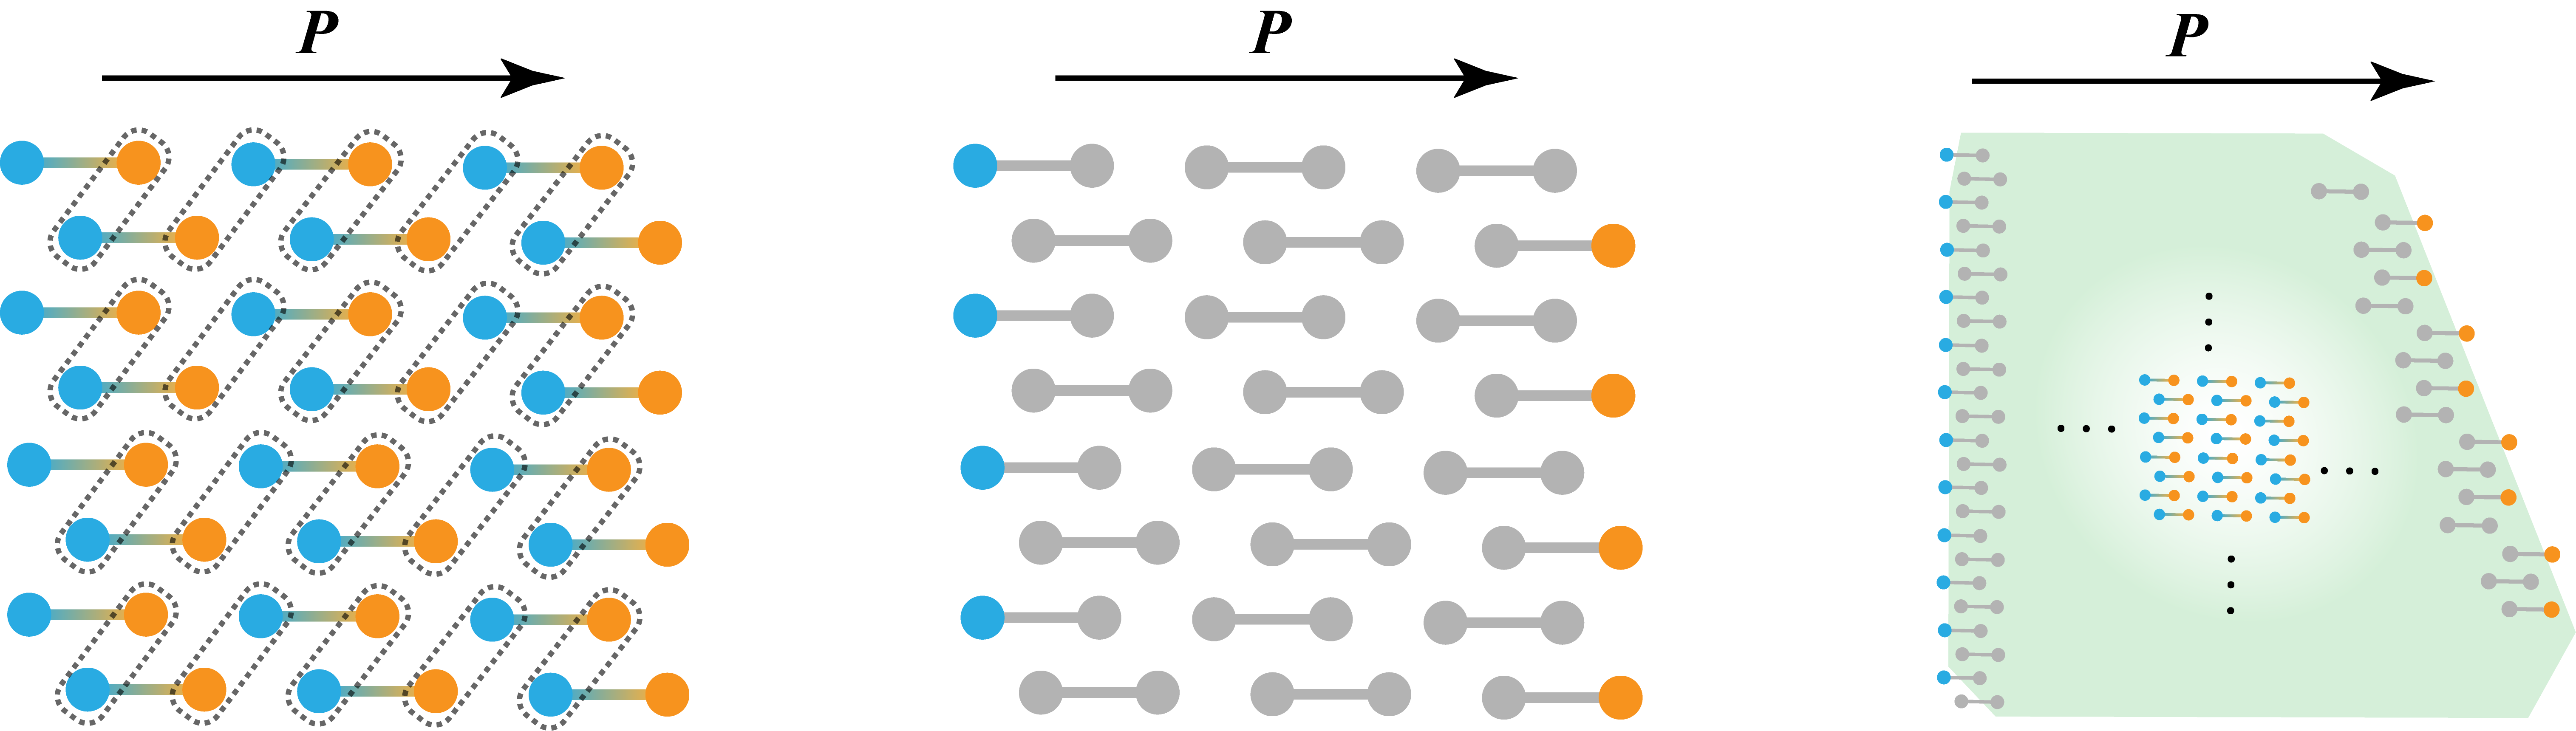
\includegraphics[width=0.9\textwidth]{image/7-1-16.png}
\caption{极化强度导致表面面电荷分布}
\end{figure}

从以上表达式看得出来,\,最后电势有一种等效的求法,\,就是认为在体内有一个$\rho_P=-\nabla'\cdot\bs{P}$的电荷密度分布,\,而认为在体表面的面元$\ud \bs{A}$上带有面电荷$\ud Q=\bs{P}\cdot\ud \bs{A}$,\,或者认为有面电荷密度$\sigma_P=\bs{P}\cdot\bs{n}$,\,其中$\bs{n}$为体积表面的外法向量.\,与其说这是一种等效,\,不如说这只是对实际情况的另一种理解.\,如上图所示,\,这是一块均匀极化的介质,\,我们这样理解介质表面上会出现的电荷:\,对介质内部的电荷进行合适的分组使得一对一对的正负电荷产生的场互相抵消.\,这样便只剩下了表面的电荷能产生场了.\,在几何学上不难证明,\,如果电偶极子长$l$,\,两电荷为$q$,\,体密度为$n$,\,那么在与极化矢量平行的方向看两端未配对电荷的面密度恰好为$\sigma=nql=np=P$.\,再考虑面可能的倾斜便容易发现以上极化电荷面密度$\sigma_P$的公式.\,类似地,\,体电荷密度$\rho_P$对应于沿某方向的$\bs{P}$分量在变化的情形.\,具体的物理图像也请读者加以分析与思考.

我们有把握预期空间各处的电场强度的公式,\,也可以通过上述方式等效,\,毕竟我们可以通过电势计算电场:
\[\bs{E}=\oint\limits_{\partial V'} \ke \frac{\sigma_P\ud A'}{|\bs{R}|^2}\bs{e}_{\bs{R}}+\int\limits_{V'}\ke\frac{\rho_P \ud V'}{|\bs{R}|^2}\bs{e}_{\bs{R}}\]

然而,\,若要开始考虑电偶极子在场中受到的外力,\,那就势必要考虑连续分布的电荷体系产生的电场和微观非均匀分布的电荷体系的局部场之间的区别.\,我们会惊人地发现以上电场只能作为平均意义下的\emph{宏观场}(macroscopic field)而区别于电偶极子具体感受到的\emph{局域场}(local field).\,首先让我们来计算一个概念,\,一个球体内的平均场强$\overline{\bs{E}}$.\,它会计算球体内电荷的受力提供关键线索.\,以原点为中心,\,半径为$R$的球内积分直接得到:
\[\overline{\bs{E}}=\left.\int\limits_{\rm Ball}\bs{E} \ud V\right/ \frac{4}{3}\pi R^3\]

直接计算会具有相当的难度.\,这里采用的技巧是在分子积分中引入$\rho'$常数,\,把积分看做原来的电荷体系产生的电场与均匀分布在这个球体内部的电荷体系之间的相互作用力\footnote{数学上相当于把$1$视作$\bs{r}$的散度的$1/3$,\,即:
\[\nabla\cdot \bs{r}=\frac{\partial x}{\partial x}+\frac{\partial y}{\partial y}+\frac{\partial z}{\partial z}=3\]
}.\,这样的球体产生的电场强度为:
\[\bs{E}'=\begin{cases} \frac{\rho' r}{3\varepsilon_0}\bs{e}_r & (r<R)\\[4pt] \frac{\rho' R^3}{3\varepsilon_0 r^2}\bs{e}_r & (r>R) \end{cases}\]

从而上式被等价写作:
\[\overline{\bs{E}}=\left.\int\limits_{\rm Ball}\rho' \bs{E} \ud V\right/ \frac{4}{3}\pi \rho' R^3=\left.\int\limits_{\rm Ball} \bs{E}\nabla\cdot\bs{E}'  \ud V\right/ \frac{4}{3}\pi \rho' R^3=\left.\int\limits_{\rm all} \bs{E}\nabla\cdot\bs{E}'  \ud V\right/ \frac{4}{3}\pi \rho' R^3\]

最后一步${\rm all}$改为对全空间积分.\,由牛顿第三定律,\,几乎可以肯定上式通过某种化简\footnote{数学上需要用到张量分析,\,过程略去.}后可以得到作用力与反作用力和为零的结论:
\[\int\limits_{\rm all} \bs{E}\nabla\cdot\bs{E}'  \ud V+\int\limits_{\rm all} \bs{E}'\nabla\cdot\bs{E}  \ud V=\bs{0}\]

于是把原电场对应的电荷密度记做$\rho$,\,待求的量变成:
\[\overline{\bs{E}}=-\left.\int\limits_{\rm all}\rho \bs{E}' \ud V\right/ \frac{4}{3}\pi \rho' R^3=\ke\frac{-\int\limits_{\rm Ball}\rho \bs{r}\ud V}{R^3}+\int\limits_{\rm all-Ball}\ke\frac{\rho(-\bs{e}_r)}{r^2}\ud V\]

\begin{figure}[H]
\centering
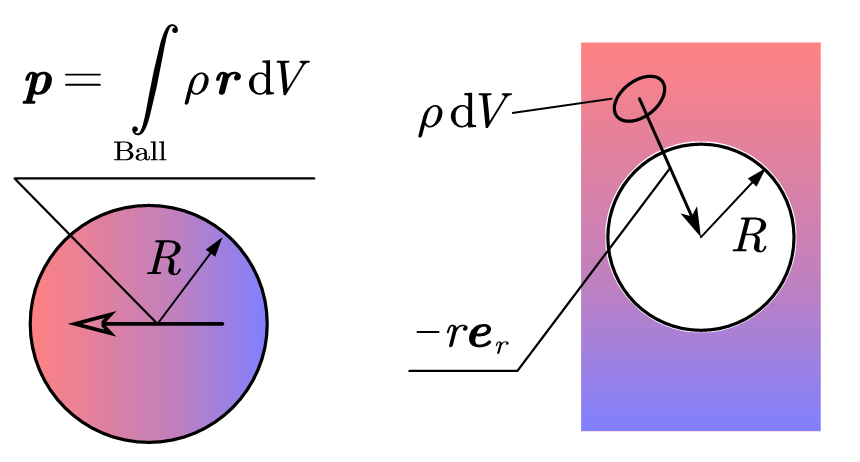
\includegraphics[width=0.6\textwidth]{image/7-1-17.png}
\caption{球内平均电场的两项积分}
\end{figure}

通过以上结果我们发现,\,在一个电荷分布体系中的一个球体内的平均电场取决于两项积分.\,第一项不是别的,\,就是直接取决于球内电荷分布产生的电偶极矩$\bs{p}$.\,第二项则代表外界电荷直接对球心处产生的电场\footnote{这意味着如果球内没有电荷,\,那么对球内电场做平均的结果恰好得到球心处电场.\,这种性质称作\emph{调和}(harmonic).}.

接下来可以进行以下推演:\,如果外界电荷不是那么紧密地靠近球面,\,那么我们可以通过球面把电荷体系分为两部分.\,现在我们来关心内部这些电荷的受力.\,依然从电场考虑,\,由于外部电荷离球面较远,\,故可以近似认为在球内产生一个均匀的电场$\bs{E}_{\rm ex}$,\,甚至于它就可以近似地等于对球心处的场强,\,这样我们就把之前的式子写为:
\[\overline{\bs{E}}=\ke \frac{-\bs{p}}{R^3}+\bs{E}_{\rm ex} \quad\Rightarrow \quad \bs{E}_{\rm ex}=\overline{\bs{E}}+\ke \frac{\bs{p}}{R^3}\]

如果让求平均的体积非常小,\,而电荷又总是连续化,\,那么$\overline{\bs{E}}$又应当与之前通过极化电荷分布计算的体内点场强$\bs{E}$无异.\,我们已经观察到一个十分关键的信息:\,考虑球内电荷受力时应当使用的外界的场$\bs{E}_{\rm ex}$,\,它与忽略电荷不连续性而计算出来的``平均场''$\bs{E}$存在一个差.\,最后考虑到极化强度的定义$\bs{P}=\lim\limits_{R\to 0}\bs{p}\left/\frac{4}{3}\pi R^3\right.$,\,最终我们得到:
\[\bs{E}_{\rm ex}=\bs{E}+\frac{\bs{P}}{3\varepsilon_0}\]

这个细节对理解介质的极化十分重要.\,我们将会在下一章重新回到这个问题.

\subsection{若干对称带电体系的电场}

最后还有一些常见的带电体系的电场是值得作为现成结论去记忆的.\,它们易于计算的原因在于或多或少具有某些对称性.\,在此逐一加以回忆与讨论.

\vspace{0.3cm}
\textbf{1.}\,薄球壳:\,以球心为原点,\,三维旋转对称性.\,过球心的镜面对称性.

\[\varphi=\begin{cases} \ke \frac{Q}{R}& (r<R) \\[3pt] \ke \frac{Q}{r} & (r>R) \end{cases} \quad,	\quad \bs{E}=\begin{cases}  \bs{0} & (r<R) \\[3pt] \ke \frac{Q}{r^2}\bs{e}_r & (r>R) \end{cases}\]

我们来到第一个问题:\,球面上的场是如何的?\,我们就会遇到\emph{发散困难}(divergency difficulty).\,这时候的处理需要特定的方法.\,论电势,\,问题不大,\,从球内球外的电势数据(下面的势曲线\ref{fig7-1-18})来看,\,球面上的电势连续,\,但是其变化率不连续(不光滑).\,所以很自然地球面上电势定义为双边的极限值即球内电势$\ke \frac{Q}{R}$.\,有限面电荷情况的电势都是不存在发散困难的.\,因为在面上局部划出来一个近似均匀带电$\sigma$,\,半径为$a$小圆盘,\,则盘心电势:
\[\varphi=\int_0^a \ke \frac{\sigma \cdot 2\pi r \ud r}{r}=\frac{\sigma a}{2\varepsilon_0}\]

是一个有限值.\,而圆盘以外的电荷对圆心的电势显然也是有限的.\,故无发散困难.\,反观电场强度,\,这情况就很不一样了.\,首当其冲地从以上公式上看,\,球内球外的电场显然不连续而在球面上具有不同的极限.\,其更深层次的原因在于:\,面电荷的电场强度积分本质上是发散的,\,有\emph{奇异性}(sigularity)的.\,考虑一个均匀带电$\sigma$,\,圆心角为可近似的小角$\Delta\alpha$,\,半径$a$的扇形.\,圆心处的场强:
\[E=\int_0^a \ke \frac{\sigma \cdot \Delta \alpha r \ud r}{r^2}=\frac{\sigma\Delta\alpha}{4\pi\varepsilon_0}\ln\frac{a}{0}=\infty\]

规避掉发散\footnote{称作\emph{正规化}(regularization).}的思想有两种.\,一是通过\emph{主值积分}(principal value integral)的方式去做\emph{截断}(cutoff),\,在需要确定场强的点处挖去一个半径为$a$的球,\,计算其他部分在该点处的场强并最后让$a\to 0$;\,二是通过平均来理解发散的场强,\,如之前所说的,\,点电荷模型与连续分布的电荷模型是统一的,\,后者计算出来的场强就是前一种不均匀场强的球体平均.\,故只需要在面电荷情况也做平均就能规避发散点的计算而利用球内其他可以计算的点来计算场强.\,计算过程略去,\,但不管哪种方法,\,最后的结果都是:
\[E=\frac{Q}{8\pi\varepsilon_0 R^2}\]

\begin{figure}[H]
\centering
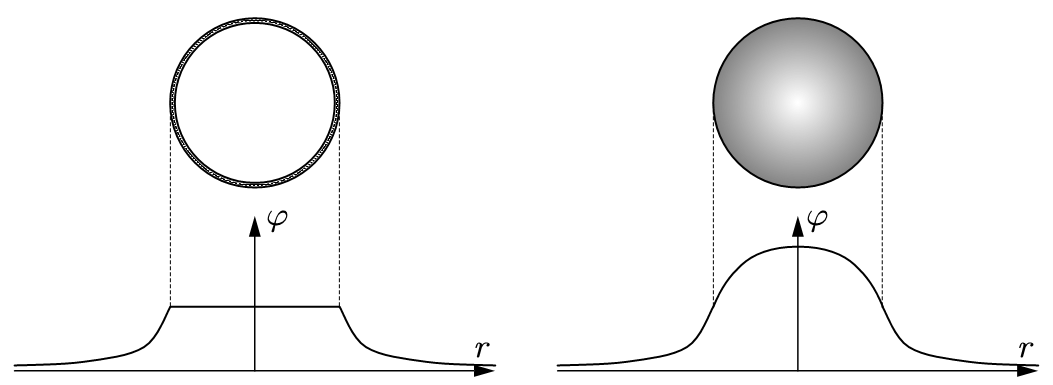
\includegraphics[width=0.7\textwidth]{image/7-1-18.png}
\caption{薄球壳与球体的势曲线}\label{fig7-1-18}
\end{figure}

\textbf{2.}\,球体:\,以球心为原点,\,三维旋转对称性.\,过球心的镜面对称性.

\[\varphi=\begin{cases} -\frac{\rho }{6\varepsilon_0}r^2+C& (r<R) \\[3pt] \ke \frac{Q}{r} & (r>R) \end{cases} \quad,	\quad \bs{E}=\begin{cases}  \frac{\rho }{3\varepsilon_0}r \bs{e}_r & (r<R) \\[3pt] \ke \frac{Q}{r^2}\bs{e}_r & (r>R) \end{cases}\]

均匀带电球体没有发散困难.\,但注意在无穷远电势为零的规范下为了使得以上电势连续,\,附加常数$C$应当为:
\[C=\frac{3Q}{8\pi\varepsilon_0 R}\]

\vspace{0.3cm}
\textbf{3.}\, 无限大带电平面:\,保持平面位置不变的平移,\,旋转对称性.\,带电平面镜像对称.\,竖直面镜像对称.

\[\varphi =-\frac{\sigma}{2\varepsilon_0}|z| \quad,\quad \bs{E}=\frac{\sigma}{2\varepsilon_0} {\rm sgn}(z)\bs{e}_z\]

其中${\rm sgn}$是\emph{符号函数}(sign function),\,即当自变量$z$取正时为$+1$,\,为负时取$-1$.\,${\rm sgn}(z)=z/|z|$.\,从计算上看,\,面上电场依然有奇异性.\,面外则通过积分的方式定义的电场奇异性消失.\,但是电势即使在面外此时也有奇异性了,\,不能通过电荷积分得到电势的值,\,只能通过与电场的关系,\,所以此时无法把无穷远作为势能的零点,\,这里的无穷远也自动被分离为下半空间无穷远和上半空间无穷远,\,所有涉及到无穷大带电平面的问题这样两个无穷远都必须要被区别对待.



\begin{figure}[H]
\centering
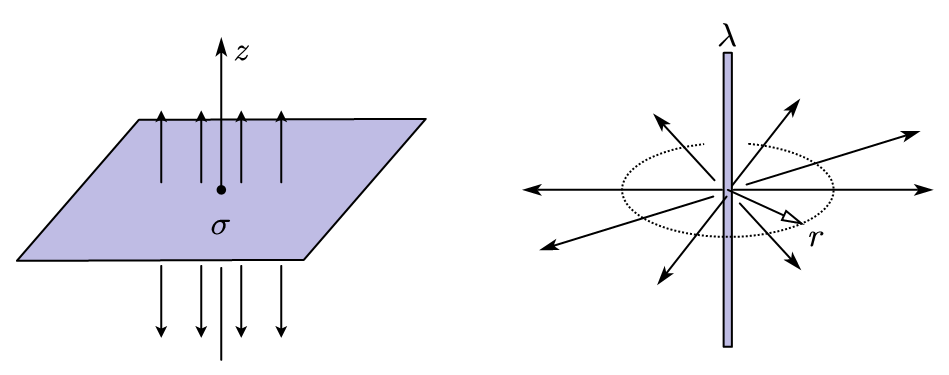
\includegraphics[width=0.7\textwidth]{image/7-1-19.png}
\caption{无限大平面与无限长直线}\label{fig7-1-19}
\end{figure}

\textbf{4.}\, 无限长带电直线:\,保持直线位置不变的平移,\,旋转对称性.\,水平面镜像对称.\,过直线的竖直面镜像对称.

\[\varphi =-\frac{\lambda}{2\pi\varepsilon_0}\ln r \quad,\quad \bs{E}=\frac{\lambda}{2\pi\varepsilon_0 r}\bs{e}_r\]

请尤其注意电势前的负号.\,同样地,\,电场在导线外是没有奇异性的,\,但是电势有奇异性,\,电势是通过与电场关系定义的,\,不能把无穷远电势视作零.\,与上一种电荷分布之所以具有不能把无穷远视作势能零点的共同点,\,是因为电荷分布的范围不是有限.\,试想在无穷远外都有电荷了怎么不可能不影响无穷远的电势分布?

如果是一个半径为$R$的,\,带电面密度为$\sigma$的圆柱薄壳,\,那么内部也将没有电场,\,等势.\,这一点从高斯定律很容易能看出来.

\vspace{0.3cm}
\textbf{5.}\, 圆环:\,旋转对称性.\,过环水平面镜像对称.\,过轴线的竖直面镜像对称.

\begin{wrapfigure}[11]{o}[0pt]{7cm}
\centering
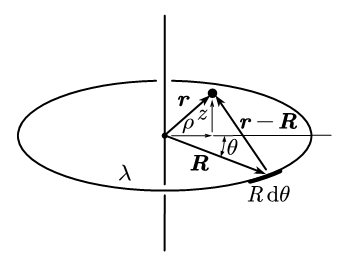
\includegraphics[width=7cm]{image/7-1-20.png}
\caption{圆环的中心附近电场}
\end{wrapfigure}
这样一个体系只有轴线上的电势和电场才有比较简单的表达式:
\[\varphi=\frac{\lambda}{2\varepsilon_0}\frac{1}{\sqrt{R^2+z^2}} \quad, \quad \bs{E}=\frac{\lambda}{2\varepsilon_0}\frac{z}{(R^2+z^2)^{\frac{3}{2}}}\bs{e}_z\]

但是实际应用场合中,\,环心附近的场也是非常需要的.\,其计算方法其实就是之前介绍的多极展开,\,不过现在需要保留到二阶项才能得到领头项:
\begin{align*}
\varphi  	&= \int \ke \frac{\ud Q}{|\bs{r}-\bs{R}|}\\
				&= \int_0^{2\pi} \ke \frac{\lambda R\ud \theta}{\sqrt{(R\cos\theta -\rho)^2+ R^2\sin^2 \theta +z^2}}\\
				\end{align*}
				\begin{align*}
				&= \int_0^{2\pi} \ke \frac{\lambda \ud \theta}{\sqrt{1+\frac{z^2+\rho^2-2R\rho\cos\theta}{R^2}}}\\
				&= \frac{\lambda}{4\pi\varepsilon_0}\int_0^{2\pi} \left(1+\frac{z^2+\rho^2-2R\rho\cos\theta}{R^2}\right)^{-\frac{1}{2}}\ud \theta\\
				&\approx \frac{\lambda}{4\pi\varepsilon_0}\int_0^{2\pi} \left[1-\frac{1}{2}\frac{z^2+\rho^2-2R\rho\cos\theta}{R^2}+\frac{3}{8}\left( \frac{z^2+\rho^2-2R\rho\cos\theta}{R^2} \right)^2 \right]\ud \theta\\
				&\approx \frac{\lambda}{4\pi\varepsilon_0}\int_0^{2\pi} \left(1+\frac{\rho\cos\theta}{R}-\frac{z^2+\rho^2}{2R^2}+\frac{3\rho^2\cos^2\theta}{2R^2} \right)\ud \theta\\
				&= \frac{\lambda}{2\varepsilon_0}\left(1-\frac{z^2}{2R^2}+\frac{\rho^2}{4R^2} \right)\\
\end{align*}

于是原点附近的场强就是这个势的梯度:
\[E_\rho=-\frac{\partial \varphi}{\partial \rho}=-\frac{\lambda}{4\varepsilon_0 R^2}\rho \quad,\quad E_z=-\frac{\partial \varphi}{\partial z}=-\frac{\lambda}{2\varepsilon_0 R^2}z\]

\begin{figure}[H]
\centering
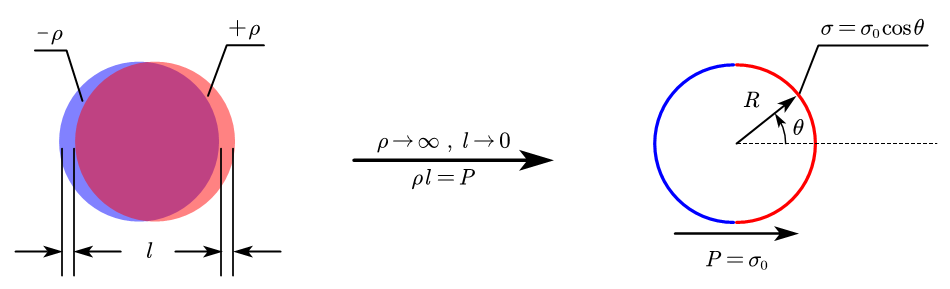
\includegraphics[width=0.7\textwidth]{image/7-1-21.png}
\caption{均匀极化的球}\label{fig7-1-21}
\end{figure}

\textbf{6.}\, 均匀极化球体.\,对极化方向的中心轴的旋转对称性,\,过轴的平面的镜像对称性.

\begin{wrapfigure}[11]{o}[0pt]{5cm}
\vspace{-0.4cm}
\centering
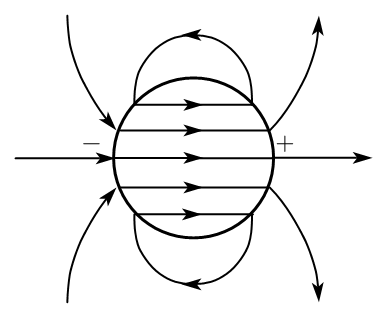
\includegraphics[width=5cm]{image/7-1-22.png}
\caption{均匀极化场}
\end{wrapfigure}
设球内极化强度为$P$.\,由之前的极化强度与电荷密度的关系知道,\,这相当于一个表面带电$\sigma=\sigma_0\cos\theta$的球壳.\,但是为了计算其内外的场强,\,我们需要把极化强度还原为单位体积内携带的电偶极子的总和.\,每个电偶极子可视为一对点电荷.\,从而形成两个电荷密度分别为$+\rho$和$-\rho$的球体,\,球心沿极化方向岔开$l$.\,只需计算极限情况:
\[\rho\to \infty \quad,\quad l\to 0 \quad,\quad \rho l=P\]

定义球内的总电偶极矩$\bs{p}=\bs{P}\cdot\frac{4}{3}\pi R^3$由球对内对外的场强公式计算得,\,球内外的场强为:
\[\bs{E}=\begin{cases}
-\frac{\bs{P}}{3\varepsilon_0}&(r<R)\\[3pt]
\ke \frac{2p\cos\theta}{r^3}\bs{e}_r + \ke \frac{p\sin\theta}{r^3}\bs{e}_\theta &(r>R)
\end{cases}\]

无奇异性,\,且也可以得到电势公式:
\[\varphi=\begin{cases}
\frac{P}{3\varepsilon_0}r\cos\theta &(r<R)\\[3pt]
\ke \frac{p\cos\theta}{r^2}&(r>R)
\end{cases}\]


%\vspace{0.3cm}
%\textbf{7.}\, 均匀带电线段